\documentclass[titlepage]{article}
\usepackage[utf8]{inputenc}
\usepackage{amsmath, amssymb, amsthm}
\usepackage{algorithmicx}
\usepackage{graphicx}
\usepackage{subcaption}
\usepackage{listings}
\usepackage{color}
\usepackage{mdframed}
\usepackage{float}
\usepackage{booktabs}
\usepackage{mathtools}

\newcommand{\diag}{\operatorname{diag}}

\definecolor{dkgreen}{rgb}{0,0.6,0}
\definecolor{gray}{rgb}{0.5,0.5,0.5}
\definecolor{mauve}{rgb}{0.58,0,0.82}

\lstset{frame=single,
	language=matlab,
	aboveskip=3mm,
	belowskip=3mm,
	showstringspaces=false,
	columns=flexible,
	basicstyle={\small\ttfamily},
	numbers=none,
	numberstyle=\tiny\color{gray},
	keywordstyle=\color{blue},
	commentstyle=\color{dkgreen},
	stringstyle=\color{mauve},
	breaklines=true,
	breakatwhitespace=true,
	tabsize=3
}

\setlength{\parindent}{0pt}

\title{AAE 50700: Principles of Dynamics\\ Problem Set 9 Report}
\author{Dylan Ashby}
\date{\today}

\begin{document}

\maketitle

\section*{(a): Given}

Consider a Keplerian orbit with $e\in(0,1)$ and $i\in(0,\pi/2)$ in the spherical coordinates $\boldsymbol{q}=(r,\phi,\theta)$ as defined in class. The Hamiltonian per unit mass (specific Hamiltonian) is given by:
\begin{equation}
	H=\frac{1}{2}\left(p_r^2+\frac{p_\phi^2}{r^2\cos^2\theta}+\frac{p_\theta^2}{r^2}\right)-\frac{\mu}{r}
\end{equation}
where $\boldsymbol{p}=(p_r,p_\phi,p_\theta)$ are specific momenta. You may use the complete separability of the Keplerian motion without proof (shown in class), with $W=W_r(r,\boldsymbol{\alpha})+W_\phi(\phi,\boldsymbol{\alpha})+W_\theta(\theta,\boldsymbol{\alpha})$.

\subsection*{(a.1): Find}

Show that the separation constants and action variables are expressed as:
\begin{equation}
	\begin{aligned}
		\alpha_1 &= H < 0, & \alpha_\phi &= p_\phi > 0, & \alpha_\theta &= \sqrt{p_\theta^2 + \frac{p_\phi^2}{\cos^2\theta}}, \\
		J_r &= \frac{1}{2\pi} \oint \pm \sqrt{2\alpha_1 + \frac{2\mu}{r} - \frac{\alpha_\theta^2}{r^2}}\,\mathrm{d}r, & J_\phi &= \alpha_\phi, & J_\theta &= \alpha_\theta - \alpha_\phi.
	\end{aligned}
\end{equation}

\textbf{Analysis/Conclusions:}\\

The first step is to derive the Hamilton-Jacobi PDE for the system, using the Hamilton Jacobi equation:
\begin{equation}
	H\left(\boldsymbol{q},\nabla_{\boldsymbol{q}}S,t\right)+\frac{\partial S}{\partial t}=0
\end{equation}

Let $S(\boldsymbol{q},\boldsymbol{\alpha},t)=W(\boldsymbol{q},\boldsymbol{\alpha})-\alpha_1 t$, where $\boldsymbol{\alpha}$ replaces the conjugate momenta using generating function $W$ and $S$ is the principal function:
\begin{equation}
	H\left(\boldsymbol{q},\nabla_{\boldsymbol{q}}\left(W-\alpha_1 t\right),t\right)+\frac{\partial}{\partial t}\left(W-\alpha_1 t\right)=0
\end{equation}

Since this is a time autonomous system, $\partial H/\partial t=0$, so time dependency is removed from $H$, and the partial of $t$ evaluates to leave $\alpha_1$ behind:
\begin{equation}
	\begin{split}
		H\left(\boldsymbol{q},\nabla_{\boldsymbol{q}}W-\nabla_{\boldsymbol{q}}(\alpha_1 t)\right)+\left(\frac{\partial W}{\partial t}-\frac{\partial}{\partial t}(\alpha_1 t)\right)&=0\\
		H\left(\boldsymbol{q},\nabla_{\boldsymbol{q}}W-0\right)+\left(0-\alpha_1\right)&=0\\
		H\left(\boldsymbol{q},\nabla_{\boldsymbol{q}}W\right)&=\alpha_1
	\end{split}
	\label{eq:timeindependenthj}
\end{equation}

The problem, setup asserts we can assume the characteristic function $W$ is separable in each of the coordinates for this system. Furthermore, since we are assuming an eccentricity $e$ between $0$ and $1$, we also assume the total energy $T+V<0$ as it describes an elliptical orbit. A total energy less than $0$ means the system is periodic/quasi-periodic. Separability of $W$ plus a periodic system meet the two conditions for us to be able to solve the HJ PDE for the action angle variables. \\

So, we setup the HJ equation for the system using the given Hamiltonian and the time autonomous HJ equation by replacing the momenta $p$ with $\nabla_{\boldsymbol{q}}W$
\begin{equation}
	\begin{split}
		\alpha_1&=H \\
		\alpha_1&=\frac{1}{2}\left(p_r^2+\frac{p_\phi^2}{r^2\cos^2\theta}+\frac{p_\theta^2}{r^2}\right)-\frac{\mu}{r} \\
		2\alpha_1&=p_r^2+\frac{p_\phi^2}{r^2\cos^2\theta}+\frac{p_\theta^2}{r^2}-\frac{2\mu}{r} \\
		2\alpha_1&=\left(\frac{\partial W}{\partial r}\right)^2+\left(\frac{\partial W}{\partial\phi}\right)^2\frac{1}{r^2\cos^2\theta}+\left(\frac{\partial W}{\partial\theta}\right)^2\frac{1}{r^2}-\frac{2\mu}{r}
	\end{split}
\end{equation}

Because we assume the characteristic function is separable, we can map the conjugate momenta directly to their respective gradients of $\boldsymbol{q}$ with respective to their separated section of the characteristic equation:
\begin{equation}
	p_r=\frac{\partial W_r(r,\boldsymbol{\alpha})}{\partial r},\quad p_\phi=\frac{\partial W_\phi(\phi,\boldsymbol{\alpha})}{\partial \phi},\quad p_\theta=\frac{\partial W_\theta(\theta,\boldsymbol{\alpha})}{\partial \theta}
\end{equation}

Which also means the HJ equation only needs to evaluate each coordinate component of $W$ for the partial respective to the same coordinate:
\begin{equation}
	2\alpha_1=\left(\frac{\partial W_r}{\partial r}\right)^2+\left(\frac{\partial W_\phi}{\partial\phi}\right)^2\frac{1}{r^2\cos^2\theta}+\left(\frac{\partial W_\theta}{\partial\theta}\right)^2\frac{1}{r^2}-\frac{2\mu}{r}
\end{equation}

We know the coordinate $\phi$ is cyclic since it does not appear in the Hamiltonian $H$. Thus this means its conjugate momentum is constant, and so is the gradient of its section of the characteristic equation. Since $\partial W_\phi/\partial\phi$ is constant, we may take it as the separation constant $\alpha_\phi$, which serves as one of the new momenta:
\begin{equation}
	p_\phi=\frac{\partial W_\phi(\phi,\boldsymbol{\alpha})}{\partial \phi}=\alpha_\phi
	\label{eq:alphaphi}
\end{equation}

So, this rewrites the HJ equation as:
\begin{equation}
	\begin{split}
		2\alpha_1=\left(\frac{\partial W_r}{\partial r}\right)^2+\frac{\alpha_\phi^2}{r^2\cos^2\theta}+\left(\frac{\partial W_\theta}{\partial\theta}\right)^2\frac{1}{r^2}-\frac{2\mu}{r}
	\end{split}
\end{equation}

And then we can perform some algebra to separate out $r$ and $\theta$ to get to the right and left hand sides respectively to get:
\begin{equation}
	\begin{split}
		r^2\left(2\alpha_1\right)&=r^2\left(\left(\frac{\partial W_r}{\partial r}\right)^2+\frac{\alpha_\phi^2}{r^2\cos^2\theta}+\left(\frac{\partial W_\theta}{\partial\theta}\right)^2\frac{1}{r^2}-\frac{2\mu}{r}\right)\\
		2\alpha_1 r^2&=r^2\left(\frac{\partial W_r}{\partial r}\right)^2+\frac{r^2\alpha_\phi^2}{r^2\cos^2\theta}+\frac{r^2}{r^2}\left(\frac{\partial W_\theta}{\partial\theta}\right)^2-\frac{2\mu r^2}{r}\\
		2\alpha_1 r^2&=r^2\left(\frac{\partial W_r}{\partial r}\right)^2+\frac{\alpha_\phi^2}{\cos^2\theta}+\left(\frac{\partial W_\theta}{\partial\theta}\right)^2-2\mu r\\
		\frac{\alpha_\phi^2}{\cos^2\theta}+\left(\frac{\partial W_\theta}{\partial\theta}\right)^2&=2\alpha_1r^2+2r\mu-r^2\left(\frac{\partial W_r}{\partial r}\right)^2
	\end{split}
\end{equation}

For the HJ equation above, separated into a function of $\theta$ and a function of $r$, to remain true for all values of $\theta$ and $r$, it must hold when either variable is held constant while the other varies. When one variable is held constant, its side of the equation is also constant due to the separation of the two variables. Since the two sides are equal, the other side must also stay constant even as its variable changes. Since this must be true for both variables, both sides must be constant. \\

The constant value of these two sides of the HJ equation can take any arbitrary label. We have found a constant value from the HJ equation for both $\alpha_1$ and $\alpha_\phi$, but we still need a constant value for $\alpha_\theta$. Likewise, we equate both sides of the equation to $\alpha_\theta^2$ to give a value to this constant. The choice of squaring it was done for convenience because the $\theta$ side of the equation is a sum of squared terms, and is therefore positive, so $\alpha_\theta$ remains positive too. Since the action variables $J$ are derived using the momenta, we substitute back $p_\theta=\partial W_\theta/\partial\theta$, $p_r=\partial W_r/\partial r$, and $p_\phi=\alpha_\phi$:
\begin{equation}
	\begin{aligned}
		&\text{LHS}\\[6pt]
		&\text{RHS}
	\end{aligned}
	\left\{
	\begin{aligned}
		\alpha_\theta^2&=\frac{\alpha_\phi^2}{\cos^2\theta}+\left(\frac{\partial W_\theta}{\partial\theta}\right)^2=\frac{p_\phi^2}{\cos^2\theta}+p_\theta^2\\
		\alpha_\theta^2&=2\alpha_1r^2+2r\mu-r^2\left(\frac{\partial W_r}{\partial r}\right)^2=2\alpha_1r^2+2r\mu-r^2p_r^2
	\end{aligned}
	\right.
	\label{eq:rhslhs}
\end{equation}

From the left hand side expression above, we can then find the equation for $\alpha_\theta$:
\begin{equation}
	\begin{split}
		\alpha_\theta^2&=\frac{p_\phi^2}{\cos^2\theta}+p_\theta^2 \\
		\sqrt{\alpha_\theta^2}&=\sqrt{\frac{p_\phi^2}{\cos^2\theta}+p_\theta^2} \\
		\alpha_\theta&=\sqrt{\frac{p_\phi^2}{\cos^2\theta}+p_\theta^2}
	\end{split}
	\label{eq:alphatheta}
\end{equation}

\begin{mdframed}[linewidth=1pt, innertopmargin=10pt, innerbottommargin=10pt]
	Thus for the separation constants:\\
	
	We saw in Eq.~(\ref{eq:timeindependenthj}) that when we consider the HJ equation for a time-autonomous system, the Hamiltonian $H$ equals the first separation constant $\alpha_1$ as a natural result of the general form of the equation. We know that $H$ is equivalent to the total specific energy of the system with this construction of the Hamiltonian (mass term divided out of potential energy). We also identified that since $e\in(0,1)$, the orbits are elliptical and therefore periodic, and elliptical orbits have a negative specific energy $\mathcal{E}$. Thus this means $H=\mathcal{E}<0$ so:
	\begin{equation}
		\alpha_1=H<0
	\end{equation}
	
	Then in Eq.~(\ref{eq:alphaphi}), we determined $p_\phi=\alpha_\phi$ from the cyclic coordinate $\phi$. We know from problem set 8 that the specific momentum $p_\phi$ is equal to the specific angular momentum about the $z$ axis. This problem considers orbits of inclination $i$ between $0$ and $\pi/2$ ($0$ degrees to $90$ degrees). This means angular momentum vector will always have its $z$ component pointed in the positive direction because the orbital plane does not flip over within these bounds of $i$. This means the z component of specific angular momentum is always positive, and by extension $p_\phi$ must be positive since they are equal. Thus this means:
	\begin{equation}
		\alpha_\phi=p_\phi>0
	\end{equation}
	
	\textbf{DO I NEED TO EXPLAIN WHY h=p TA?} \\
	
	Finally in Eq.~(\ref{eq:alphatheta}) it was derived from the separability of $\theta$ and $r$ coordinates in the HJ equation that $\alpha_\theta$ has the following value:
	\begin{equation}
		\alpha_\theta=\sqrt{p_\theta^2+\frac{p_\phi^2}{\cos^2\theta}}
	\end{equation}
\end{mdframed}

We can then take the left and right hand side expressions from Eq.~(\ref{eq:rhslhs}) to get expressions for specific momenta $p_\theta$ and $p_r$:
\begin{equation}
	\begin{split}
		\alpha_\theta^2&=\frac{\alpha_\phi^2}{\cos^2\theta}+p_\theta^2 \\
		p_\theta^2&=\alpha_\theta^2-\frac{\alpha_\phi^2}{\cos^2\theta} \\
		p_\theta&=\pm\sqrt{\alpha_\theta^2-\frac{\alpha_\phi^2}{\cos^2\theta}}
	\end{split}
\end{equation}

Then for $p_r$:
\begin{equation}
	\begin{split}
		\alpha_\theta^2&=2\alpha_1r^2+2r\mu-r^2p_r^2 \\
		r^2p_r^2&=2\alpha_1r^2+2r\mu-\alpha_\theta^2 \\
		p_r^2&=2\alpha_1+\frac{2\mu}{r}-\frac{\alpha_\theta^2}{r^2} \\
		p_r&=\pm\sqrt{2\alpha_1+\frac{2\mu}{r}-\frac{\alpha_\theta^2}{r^2}}
	\end{split}
\end{equation}
\textbf{DO I NEED TO EXPLAIN WHY THE PM TA?} \\

Then the above $p_r$ and $p_\theta$ expressions as well as the $p_\phi$ expression derived in Eq.~(\ref{eq:alphaphi}) can be substituted into the action variable $J$ expressions:
\begin{equation}
	\begin{split}
		J_r&=\frac{1}{2\pi}\oint p_r\,\mathrm{d}r=\frac{1}{2\pi}\oint\pm\sqrt{2\alpha_1+\frac{2\mu}{r}-\frac{\alpha_\theta^2}{r^2}}\,\mathrm{d}r \\
		J_\phi&=\frac{1}{2\pi}\oint p_\phi\,\mathrm{d}\phi=\frac{1}{2\pi}\oint\alpha_\phi\,\mathrm{d}\phi \\
		J_\theta&=\frac{1}{2\pi}\oint p_\theta\,\mathrm{d}\theta=\frac{1}{2\pi}\oint\pm\sqrt{\alpha_\theta^2-\frac{\alpha_\phi^2}{\cos^2\theta}}\,\mathrm{d}\theta
	\end{split}
	\label{eq:actionvars}
\end{equation}

$J_r$ is already in the form requested by the problem (and its solution is given). Then, evaluation of $J_\phi$ is fairly simple. Since $\phi$ is a rotation, one complete cycle sets integration bounds from $0$ to $2\pi$:
\begin{equation}
	J_\phi=\frac{1}{2\pi}\oint\alpha_\phi\,\mathrm{d}\phi=\frac{1}{2\pi}\int_0^{2\pi}\alpha_\phi\,\mathrm{d}\phi=\frac{\alpha_\phi}{2\pi}\left[\phi\right]_0^{2\pi}=\frac{\alpha_\phi}{2\pi}\left(2\pi-0\right)=\alpha_\phi
	\label{eq:actionphi}
\end{equation}

Then, we run through the evaluation of $J_\theta$. Starting with:
\begin{equation}
	J_\theta=\pm\frac{1}{2\pi}\oint\sqrt{\alpha_\theta^2-\frac{\alpha_\phi^2}{\cos^2\theta}}\,\mathrm{d}\theta
\end{equation}

We introduce a change of variables with $\gamma$. Since we showed $\alpha_\phi$ is always positive in our system, and $\alpha_\theta$ is always positive by the definition we used for it, the change of variables is also always positive:
\begin{equation}
	\cos(\gamma)=\frac{\alpha_\phi}{\alpha_\theta}>0
\end{equation}

Then we can substitute the change of variables into the expression for $p_\theta$:
\begin{equation}
	\begin{split}
		p_\theta&=\pm\sqrt{\alpha_\theta^2-\frac{\alpha_\phi^2}{\cos^2\theta}}=\pm\sqrt{\alpha_\theta^2\left(1-\frac{\alpha_\phi^2}{\alpha_\theta^2\cos^2\theta}\right)}=\pm\alpha_\theta\sqrt{1-\left(\frac{\alpha_\phi}{\alpha_\theta}\right)^2\frac{1}{\cos^2\theta}} \\
		&=\pm\alpha_\theta\sqrt{1-\left(\cos\gamma\right)^2\frac{1}{\cos^2\theta}}=\pm\alpha_\theta\sqrt{1-\frac{\cos^2\gamma}{\cos^2\theta}}
	\end{split}
\end{equation}

Since the angle $\theta$ oscillates between $\pm\gamma$, one complete cycle can be split into four quarter-segments ($0\to\gamma$, $\gamma\to0$, $0\to-\gamma$, $-\gamma\to0$) with a symmetry between them. Thus for one complete cycle of $\theta$, we integrate between the bounds of $0$ and $\gamma$ times four:
\begin{equation}
	J_\theta=\frac{1}{2\pi}\left(4\int_{0}^{\gamma}\alpha_\theta\sqrt{1-\frac{\cos^2\gamma}{\cos^2\theta}}\,\mathrm{d}\theta\right)=\frac{2\alpha_\theta}{\pi}\int_{0}^{\gamma}\sqrt{1-\frac{\cos^2\gamma}{\cos^2\theta}}\,\mathrm{d}\theta
\end{equation}

Then we introduce another change of variables with $\psi$, and differentiate both sides to relate $\mathrm{d}\theta$ to $\mathrm{d}\psi$:
\begin{equation}
	\begin{split}
		\sin(\theta)&=\sin(\gamma)\sin(\psi) \\
		\cos(\theta)\mathrm{d}\theta&=\sin(\gamma)\cos(\psi)\mathrm{d}\psi \\
		\mathrm{d}\theta&=\frac{\sin(\gamma)\cos(\psi)}{\cos(\theta)}\mathrm{d}\psi
	\end{split}
\end{equation}

Then we substitute back into the integral (ignoring the constant pulled outside the integral for now):
\begin{equation}
	\begin{split}
		&=\int_{0}^{\gamma}\sqrt{1-\frac{\cos^2\gamma}{\cos^2\theta}}\,\mathrm{d}\theta \\
		&=\int_{0}^{\gamma}\sqrt{\frac{\cos^2\theta}{\cos^2\theta}-\frac{\cos^2\gamma}{\cos^2\theta}}\,\mathrm{d}\theta \\
		&=\int_{0}^{\gamma}\sqrt{\frac{\cos^2\theta-\cos^2\gamma}{\cos^2\theta}}\,\mathrm{d}\theta \\
		&=\int_{0}^{\pi/2}\sqrt{\frac{\cos^2\theta-\cos^2\gamma}{\cos^2\theta}}\,\frac{\sin\gamma\cos\psi}{\cos\theta}\,\mathrm{d}\psi \\
		&=\int_{0}^{\pi/2}\frac{\sqrt{\cos^2\theta-\cos^2\gamma}}{\sqrt{\cos^2\theta}}\,\frac{\sin\gamma\cos\psi}{\cos\theta}\,\mathrm{d}\psi \\
		&=\int_{0}^{\pi/2}\frac{\sqrt{\cos^2\theta-\cos^2\gamma}}{\cos\theta}\,\frac{\sin\gamma\cos\psi}{\cos\theta}\,\mathrm{d}\psi \\
		&=\int_{0}^{\pi/2}\frac{\sin\gamma\cos\psi\sqrt{\cos^2\theta-\cos^2\gamma}}{\cos\theta\cos\theta}\,\mathrm{d}\psi \\
		&=\int_{0}^{\pi/2}\frac{\sin\gamma\cos\psi}{\cos^2\theta}\sqrt{\cos^2\theta-\cos^2\gamma}\,\mathrm{d}\psi \\
		&=\int_{0}^{\pi/2}\frac{\sin\gamma\cos\psi}{1-\sin^2\theta}\sqrt{\left(1-\sin^2\theta\right)-\left(1-\sin^2\gamma\right)}\,\mathrm{d}\psi
	\end{split}
\end{equation}

And apply the substitution again to get:
\begin{equation}
	\int_{0}^{\pi/2}\frac{\sin\gamma\cos\psi}{1-\sin^2\gamma\sin^2\psi}\sqrt{\left(1-\sin^2\gamma\sin^2\psi\right)-\left(1-\sin^2\gamma\right)}\,\mathrm{d}\psi
\end{equation}

Then we can further simplify:
\begin{equation}
	\begin{split}
		&=\int_{0}^{\pi/2}\frac{\sin\gamma\cos\psi}{1-\sin^2\gamma\sin^2\psi}\sqrt{\left(1-\sin^2\gamma\sin^2\psi\right)-\left(1-\sin^2\gamma\right)}\,\mathrm{d}\psi \\
		&=\int_{0}^{\pi/2}\frac{\sin\gamma\cos\psi}{1-\sin^2\gamma\sin^2\psi}\sqrt{1-1-\sin^2\gamma\sin^2\psi+\sin^2\gamma}\,\mathrm{d}\psi \\
		&=\int_{0}^{\pi/2}\frac{\sin\gamma\cos\psi}{1-\sin^2\gamma\sin^2\psi}\sqrt{\sin^2\gamma-\sin^2\gamma\sin^2\psi}\,\mathrm{d}\psi \\
		&=\int_{0}^{\pi/2}\frac{\sin\gamma\cos\psi}{1-\sin^2\gamma\sin^2\psi}\sqrt{\sin^2\gamma\left(1-\sin^2\psi\right)}\,\mathrm{d}\psi \\
		&=\int_{0}^{\pi/2}\frac{\sin\gamma\cos\psi}{1-\sin^2\gamma\sin^2\psi}\sqrt{\sin^2\gamma\cos^2\psi}\,\mathrm{d}\psi \\
		&=\int_{0}^{\pi/2}\frac{\sin\gamma\cos\psi}{1-\sin^2\gamma\sin^2\psi}\left(\sin\gamma\cos\psi\right)\mathrm{d}\psi \\
		&=\int_{0}^{\pi/2}\frac{\sin^2\gamma\cos^2\psi}{1-\sin^2\gamma\sin^2\psi}\,\mathrm{d}\psi
	\end{split}
\end{equation}

Then we introduce another change of variables with $u$, and differentiate both sides to relate $\mathrm{d}\psi$ to $\mathrm{d}u$:
\begin{equation}
	\begin{split}
		u&=\tan\psi \\
		\mathrm{d}u&=\frac{1}{\cos^2\psi}\mathrm{d}\psi \\
		\mathrm{d}\psi&=\cos^2\psi\,\mathrm{d}u
	\end{split}
\end{equation}

Then, a couple relations of the $\psi$ terms in the integral are made to $u$ to help with the substitution:
\begin{equation}
	\begin{split}
		\cos^2\psi&=\frac{1}{\sec^2\psi}=\frac{1}{1+\tan^2\psi}=\frac{1}{1+u^2} \\
		\sin^2\psi&=\tan^2\psi\cos^2\psi=\frac{u^2}{1+u^2}
	\end{split}
\end{equation}

Then we substitute back into the integral:
\begin{equation}
	\begin{split}
		&=\int_{0}^{\pi/2}\frac{\sin^2\gamma\cos^2\psi}{1-\sin^2\gamma\sin^2\psi}\,\mathrm{d}\psi \\
		&=\int_{0}^{\infty}\frac{\sin^2\gamma\cos^2\psi}{1-\sin^2\gamma\sin^2\psi}\left(\cos^2\psi\,\mathrm{d}u\right) \\
		&=\sin^2\gamma\int_{0}^{\infty}\frac{(\cos^2\psi)^2}{1-\sin^2\gamma\sin^2\psi}\,\mathrm{d}u \\
		&=\sin^2\gamma\int_{0}^{\infty}\left(\cos^2\psi\right)^2\frac{1}{1-\sin^2\gamma\sin^2\psi}\,\mathrm{d}u \\
		&=\sin^2\gamma\int_{0}^{\infty}\left(\frac{1}{1+u^2}\right)^2\frac{1}{1-\sin^2\gamma\frac{u^2}{1+u^2}}\,\mathrm{d}u \\
		&=\sin^2\gamma\int_{0}^{\infty}\left(\frac{1}{1+u^2}\right)^2\frac{1}{1-\sin^2\gamma\frac{u^2}{1+u^2}}\frac{1+u^2}{1+u^2}\,\mathrm{d}u \\
		&=\sin^2\gamma\int_{0}^{\infty}\frac{1+u^2}{\left(1+u^2\right)^2}\frac{1}{(1+u^2)(1-\sin^2\gamma\frac{u^2}{1+u^2})}\,\mathrm{d}u \\
		&=\sin^2\gamma\int_{0}^{\infty}\frac{1}{1+u^2}\frac{1}{1+u^2-u^2\sin^2\gamma}\,\mathrm{d}u \\
		&=\sin^2\gamma\int_{0}^{\infty}\frac{1}{1+u^2}\frac{1}{1+u^2\left(1-\sin^2\gamma\right)}\,\mathrm{d}u \\
		&=\sin^2\gamma\int_{0}^{\infty}\frac{1}{(1+u^2)(1+u^2\cos^2\gamma)}\,\mathrm{d}u
	\end{split}
\end{equation}

Then we can use partial fraction decomposition to separate the two parts of the denominator:
\begin{equation}
	\begin{split}
		\frac{1}{(1+u^2)(1+u^2\cos^2\gamma)}&=\frac{A}{1+u^2}+\frac{B}{1+u^2\cos^2\gamma} \\
		1&=A\left(1+u^2\cos^2\gamma\right)+B\left(1+u^2\right) \\
		1&=(A+B)+(A\cos^2\gamma+B)u^2 \\
		&\implies A+B=1,\quad A\cos^2\gamma+B=0 \\
		&\implies A=\frac{1}{1-\cos^2\gamma}=\frac{1}{\sin^2\gamma},\quad B=-\frac{\cos^2\gamma}{\sin^2\gamma} \\
		\frac{A}{1+u^2}+\frac{B}{1+u^2\cos^2\gamma}&=\left(\frac{1}{\sin^2\gamma}\right)\frac{1}{1+u^2}+\left(-\frac{\cos^2\gamma}{\sin^2\gamma}\right)\frac{1}{1+u^2\cos^2\gamma} \\
		&=\frac{1}{\sin^2\gamma}\left(\frac{1}{1+u^2}-\frac{\cos^2\gamma}{1+u^2\cos^2\gamma}\right)
	\end{split}
\end{equation}

So, then we substitute the decomposition back into the integral:
\begin{equation}
	\begin{split}
		&=\sin^2\gamma\int_{0}^{\infty}\frac{1}{(1+u^2)(1+u^2\cos^2\gamma)}\,\mathrm{d}u \\
		&=\sin^2\gamma\int_{0}^{\infty}\frac{1}{\sin^2\gamma}\left(\frac{1}{1+u^2}-\frac{\cos^2\gamma}{1+u^2\cos^2\gamma}\right)\mathrm{d}u \\
		&=\frac{\sin^2\gamma}{\sin^2\gamma}\int_{0}^{\infty}\left(\frac{1}{1+u^2}-\frac{\cos^2\gamma}{1+u^2\cos^2\gamma}\right)\mathrm{d}u \\
		&=\int_{0}^{\infty}\left(\frac{1}{1+u^2}-\frac{\cos^2\gamma}{1+u^2\cos^2\gamma}\right)\mathrm{d}u \\
		&=\int_{0}^{\infty}\frac{1}{1+u^2}\,\mathrm{d}u-\int_{0}^{\infty}\frac{\cos^2\gamma}{1+u^2\cos^2\gamma}\,\mathrm{d}u \\
		&=\int_{0}^{\infty}\frac{1}{1+u^2}\,\mathrm{d}u-\cos^2\gamma\int_{0}^{\infty}\frac{1}{1+u^2\cos^2\gamma}\,\mathrm{d}u
	\end{split}
\end{equation}

Then we can evaluate the two resulting integrals individually:
\begin{equation}
	\int_{0}^{\infty}\frac{1}{1+u^2}\,\mathrm{d}u=\Big[\arctan(u)\Big]_{0}^{\infty}=\frac{\pi}{2}-0=\frac{\pi}{2}
\end{equation}

And the other half:
\begin{equation}
	\int_{0}^{\infty}\frac{1}{1+u^2\cos^2\gamma}\,\mathrm{d}u=\frac{1}{\cos\gamma}\Big[\arctan\left(\frac{u}{\cos\gamma}\right)\Big]_{0}^{\infty}=\frac{1}{\cos\gamma}\left(\frac{\pi}{2}-0\right)=\frac{1}{\cos\gamma}\frac{\pi}{2}
\end{equation}

So, we then substitute back into the original integral to get:
\begin{equation}
	\int_{0}^{\gamma}\sqrt{1-\frac{\cos^2\gamma}{\cos^2\theta}}\,\mathrm{d}\theta=\frac{\pi}{2}-\frac{\cos^2\gamma}{\cos\gamma}\frac{\pi}{2}=\frac{\pi}{2}-\cos\gamma\frac{\pi}{2}
\end{equation}

Then we return to the action variable expression:
\begin{equation}
	J_\theta=\frac{2\alpha_\theta}{\pi}\int_{0}^{\gamma}\sqrt{1-\frac{\cos^2\gamma}{\cos^2\theta}}\,\mathrm{d}\theta=\frac{2\alpha_\theta}{\pi}\left(\frac{\pi}{2}-\cos\gamma\frac{\pi}{2}\right)=\alpha_\theta-\alpha\theta\cos\gamma
\end{equation}

Then we reuse the change of variables $\cos\gamma=\alpha_\phi/\alpha_\theta$:
\begin{equation}
	J_\theta=\alpha_\theta-\alpha_\theta\cos\gamma=\alpha_\theta-\alpha_\theta\frac{\alpha_\phi}{\alpha_\theta}=\alpha_\theta-\alpha_\phi
	\label{eq:actiontheta}
\end{equation}

\newpage

\begin{mdframed}[linewidth=1pt, innertopmargin=10pt, innerbottommargin=10pt]
	So, Eq.~(\ref{eq:actionvars}) put $J_r$ in the form requested by the problem already, Eq.~(\ref{eq:actionphi}) found the $J_\phi$ expression, and Eq.~(\ref{eq:actiontheta}) completed the derivation for $J_\theta$. Between these three equation we confirmed that:
	\begin{equation}
		J_r=\frac{1}{2\pi}\oint\pm\sqrt{2\alpha_1+\frac{2\mu}{r}-\frac{\alpha_\theta^2}{r^2}}\,\mathrm{d}r,\qquad J_\phi=\alpha_\phi,\qquad J_\theta=\alpha_\theta-\alpha_\phi
	\end{equation}
\end{mdframed}

\subsection*{(a.2): Find}

The Delaunay actions are defined as $L_D=J_r+J_\phi+J_\theta$, $G_D=J_\phi+J_\theta$, and $H_D=J_\phi$. Show that they are equivalently expressed as:
\begin{equation}
	L_D=\sqrt{\mu a},\quad G_D=L_D\sqrt{1-e^2},\quad H_D=G_D\cos i
\end{equation}
Where $a$, $e$, $i$ are subset of the classical orbital elements. \\

\textbf{Analysis/Conclusions:}\\

The problem set gives the solution to $J_r$ directly as:
\begin{equation}
	J_r=\frac{\mu}{\sqrt{-2\alpha_1}}-\alpha_\theta
\end{equation}

Then, recall the values for $J_\phi$ and $J_\theta$ are:
\begin{equation}
	J_\phi=\alpha_\phi,\quad J_\theta=\alpha_\theta-\alpha_\phi
\end{equation}

So, plugged into the definitions of Delaunay actions, we get:
\begin{equation}
	\begin{split}
		L_D&=J_r+J_\phi+J_\theta=\frac{\mu}{\sqrt{-2\alpha_1}}-\alpha_\theta+\alpha_\phi+\alpha_\theta-\alpha_\phi=\frac{\mu}{\sqrt{-2\alpha_1}} \\
		G_D&=J_\phi+J_\theta=\alpha_\phi+\alpha_\theta-\alpha_\phi=\alpha_\theta \\
		H_D&=J_\phi=\alpha_\phi
	\end{split}
\end{equation}

Then we substitute in the found values for the separation constants in (a.1):
\begin{equation}
	\begin{split}
		L_D&=\frac{\mu}{\sqrt{-2\alpha_1}}=\frac{\mu}{\sqrt{-2H}} \\
		G_D&=\alpha_\theta=\sqrt{p_\theta^2 + \frac{p_\phi^2}{\cos^2\theta}}\\
		H_D&=\alpha_\phi=p_\phi 
	\end{split}
\end{equation}

Then we substitute the Hamiltonian $H$ into $L_D$ using the given $H=-\mu/(2a)$:
\begin{equation}
	L_D=\frac{\mu}{\sqrt{-2H}}=\frac{\mu}{\sqrt{-2\left(-\frac{\mu}{2a}\right)}}=\frac{\mu}{\sqrt{\frac{\mu}{a}}}=\mu\sqrt{\frac{a}{\mu}}=\sqrt{\mu^2}\sqrt{\frac{a}{\mu}}=\sqrt{\frac{\mu^2a}{\mu}}=\sqrt{\mu a}
\end{equation}
\textbf{DO I NEED TO PROVE HAMILTONIAN EQUALS WHATS GIVEN?} \\

Then we substitute $p_\theta$ and $p_\phi$ into $G_D$ using the given $p_\theta=r^2\dot{\theta}$ and $p_\phi=r^2\cos^2\theta\,\dot{\phi}$:
\begin{equation}
	\begin{split}
		G_D&=\sqrt{p_\theta^2+\frac{p_\phi^2}{\cos^2\theta}}=\sqrt{\left(r^2\dot{\theta}\right)^2+\frac{\left(r^2\cos^2\theta\,\dot{\phi}\right)^2}{\cos^2\theta}}=\sqrt{r^4\dot{\theta}^2+r^4\cos^2\theta\,\dot{\phi}^2} \\
		&=\sqrt{r^4}\sqrt{\dot{\theta}^2+\cos^2\theta\,\dot{\phi}^2}=r^2\sqrt{\dot{\theta}^2+\cos^2\theta\,\dot{\phi}^2}
	\end{split}
\end{equation}

\textbf{IM NOT SURE WHAT TO DO HERE} \\

\subsection*{(a.3): Find}

Denote the canonical angles conjugate to $(L_D,G_D,H_D)$ by $(\ell,g,h)$. It is known that $(\ell,g,h)$ correspond to classical orbital elements as: $(\ell,g,h)=(M,\omega,\Omega)$. Express $H$ in terms of the Delaunay variables and derive the action and angle rates. Verify that $\dot{M}$ equals the Keplerian mean motion and explain what the remaining rates imply about the size, shape, and orientation of the orbit. \\

\textbf{Analysis/Conclusions:}\\

To put $H$ in terms of the Delaunay variables, recall that:
\begin{equation}
	L_D=\frac{\mu}{\sqrt{-2H}}
\end{equation}

Then putting it in terms of $H$:
\begin{equation}
	L_D=\frac{\mu}{\sqrt{-2H}}\quad\implies\quad \sqrt{-2H}=\frac{\mu}{L_D}\quad\implies\quad -2H=\frac{\mu^2}{L_D^2}\quad\implies\quad H=-\frac{\mu^2}{2L_D^2}
\end{equation}

\begin{mdframed}[linewidth=1pt, innertopmargin=10pt, innerbottommargin=10pt]
	The action rates are derived by the following equations adapted from Hamilton's equations:
	\begin{equation}
		\begin{split}
			\dot{L}_D&=-\frac{\partial H}{\partial\ell}=-\frac{\partial}{\partial\ell}\left(-\frac{\mu^2}{2L_D^2}\right)=0 \\
			\dot{G}_D&=-\frac{\partial H}{\partial g}=-\frac{\partial}{\partial g}\left(-\frac{\mu^2}{2L_D^2}\right)=0 \\
			\dot{H}_D&=-\frac{\partial H}{\partial h}=-\frac{\partial}{\partial h}\left(-\frac{\mu^2}{2L_D^2}\right)=0
		\end{split}
	\end{equation}
	
	And the angle rates are derived by the following equations adapted from Hamilton's equations:
	\begin{equation}
		\begin{split}
			\dot{\ell}&=\frac{\partial H}{\partial L_D}=\frac{\partial}{\partial L_D}\left(-\frac{\mu^2}{2L_D^2}\right)=-\frac{\mu^2}{2}\frac{\partial}{\partial L_D}\left(L_D^{-2}\right)=-\frac{\mu^2}{2}\left(-2L_D^{-3}\right)= \\
			&=\frac{2\mu^2}{2L_D^3}=\frac{\mu^2}{L_D^3} \\
			\dot{g}&=\frac{\partial H}{\partial G_D}=\frac{\partial}{\partial G_D}\left(-\frac{\mu^2}{2L_D^2}\right)=0 \\
			\dot{h}&=\frac{\partial H}{\partial H_D}=\frac{\partial}{\partial H_D}\left(-\frac{\mu^2}{2L_D^2}\right)=0
		\end{split}
	\end{equation}
	And we see that since $H$ is only a function of $L_D$, the only non-zero rate is $\dot{\ell}$.
\end{mdframed}

From the problem definition, we know that the angle variable $\ell$ is equal to the mean anomaly $M$. Which then implies that $\dot{\ell}=\dot{M}$. The derivative for mean anomaly is equal to mean motion $n$. The expression for Keplerian mean motion is:
\begin{equation}
	n=\sqrt{\frac{\mu}{a^3}}
\end{equation}

\begin{mdframed}[linewidth=1pt, innertopmargin=10pt, innerbottommargin=10pt]
	Recall from (a.2) that $L_D=\sqrt{\mu a}$, so we then see that:
	\begin{equation}
		\dot{\ell}=\dot{M}=\frac{\mu^2}{L_D^3}=\frac{\mu^2}{\left(\sqrt{\mu a}\right)^3}=\frac{\mu^2}{\left(\mu a\right)^{3/2}}=\frac{\mu^2}{\mu^{3/2}a^{3/2}}=\frac{\mu^{1/2}}{a^{3/2}}=\sqrt{\frac{\mu}{a^3}}=n
	\end{equation}
	Which proves that $\dot{M}$ is equal to mean motion $n$.
\end{mdframed}

\newpage

\begin{mdframed}[linewidth=1pt, innertopmargin=10pt, innerbottommargin=10pt]
	We see above that the remaining action and angle rates all equal zero:
	\begin{equation}
		\dot{L}_D=\dot{G}_D=\dot{H}_D=\dot{g}=\dot{h}=0
	\end{equation}
	Which mean these values are constant.
	
	Since $L_D=\sqrt{\mu a}$, $\mu$ is also a constant so a constant $L_D$ also implies a constant semi-major axis $a$. Furthermore, since $G_D=L_D\sqrt{1-e^2}$, a constant $L_D$ and $G_D$ mean eccentricity $e$ is also constant. A constant $a$ and $e$ \textbf{imply a constant size and shape of the orbit}.\\
	
	Then, since $H_D=G_D\cos i$, a constant $G_D$ and $H_D$ mean inclination $i$ is also constant. Since $g$ and $h$ equal Argument of Periapsis $\omega$, and Right Ascension of the Ascending Node $\Omega$ respectively, constant $g$ and $h$ mean a constant $\omega$ and $\Omega$. A constant $i$, $\omega$, and $\Omega$ \textbf{imply a constant orientation of the orbit}.
\end{mdframed}

\newpage

\section*{(b): Given}

Assume that the Moon follows a prescribed circular orbit. Use an inertial Earth-centered frame with the positive $z$ axis along the Moon's orbital angular momentum. \\

Let $\boldsymbol{r}$ denote the spacecraft position and $\boldsymbol{R}(t)$ the Moon's position. Taking $\boldsymbol{q}=\boldsymbol{r}$, the specific Hamiltonian is given by:
\begin{equation}
	H(\boldsymbol{q},\boldsymbol{p},t)=\frac{1}{2}\|\boldsymbol{p}\|_2^2+V(\boldsymbol{q},t),\qquad\boldsymbol{p}=\dot{\boldsymbol{q}}
\end{equation}
\begin{equation}
	V(\boldsymbol{q},t)=-\frac{\mu}{\|\boldsymbol{q}\|_2}-\frac{\mu_M}{\|\boldsymbol{R}(t)-\boldsymbol{q}\|_2}+\frac{\mu_M}{d_M^3}\boldsymbol{q}\cdot\boldsymbol{R}(t)
\end{equation}
\begin{equation}
	\boldsymbol{R}(t)=d_M
	\begin{bmatrix}
		\cos(n_Mt+\phi_M) \\
		\sin(n_Mt+\phi_M) \\
		0
	\end{bmatrix},\qquad n_M=\sqrt{\frac{\mu+\mu_M}{d_M^3}}
\end{equation}
where use the following constants:
\begin{equation}
	\mu=398600\ \mathrm{km^3/s^2},\quad\mu_M=4902.8\ \mathrm{km^3/s^2},\quad d_M=384400\ \mathrm{km},\quad\phi_M=\pi/4
\end{equation}

Assume that the spacecraft is initially at the periapsis of a GEO-scale orbit with $a=42164$ km, $e=0.01$, $i=20^\circ$, and $M=\omega=\Omega=0$. The angles are measured in the frame defined above.

\subsection*{(b.1): Find}

Verify that the lunar terms in $-\nabla_{\boldsymbol{q}}V$ (those involving $\mu_M$) reproduce the third-body perturbing acceleration covered in the review slides. \\

\textbf{Analysis/Conclusions:}\\

The third-body perturbing acceleration from the review slides is:
\begin{equation}
	\boldsymbol{a}_i=-\mu_i\left(\frac{\boldsymbol{r}-\boldsymbol{r}_i}{\|\boldsymbol{r}-\boldsymbol{r}_i\|_2^3}+\frac{\boldsymbol{r}_i}{\|\boldsymbol{r}_i\|_2^3}\right)
\end{equation}

Using the lunar terms in place of $i$ terms, and the fact that $\boldsymbol{r}=\boldsymbol{q}$, it writes as:
\begin{equation}
	\boldsymbol{a}_M=-\mu_M\left(\frac{\boldsymbol{q}-\boldsymbol{R}}{\|\boldsymbol{q}-\boldsymbol{R}\|_2^3}+\frac{\boldsymbol{R}}{\|\boldsymbol{R}\|_2^3}\right)
\end{equation}

The lunar terms of the potential are:
\begin{equation}
	V_M(\boldsymbol{q},t)=-\frac{\mu_M}{\|\boldsymbol{R}(t)-\boldsymbol{q}\|_2}+\frac{\mu_M}{d_M^3}\boldsymbol{q}\cdot\boldsymbol{R}(t)
\end{equation}

The gradient of a norm of a vector with respect to itself is equal to the unit vector of that vector:
\begin{equation}
	\frac{\partial\|\boldsymbol{v}\|_2}{\partial\boldsymbol{v}}=\frac{\boldsymbol{v}}{\|\boldsymbol{v}\|_2}
\end{equation}

Taking the gradient of the first term with the chain rule, and the above stated rule for gradients of vector norms:
\begin{equation}
	\begin{split}
		&=\frac{\partial}{\partial\boldsymbol{q}}\left(-\frac{\mu_M}{\|\boldsymbol{R}-\boldsymbol{q}\|_2}\right) \\
		&=\frac{\partial}{\partial\|\boldsymbol{R}-\boldsymbol{q}\|_2}\left(-\frac{\mu_M}{\|\boldsymbol{R}-\boldsymbol{q}\|_2}\right)\frac{\partial\|\boldsymbol{R}-\boldsymbol{q}\|_2}{\partial\boldsymbol{q}} \\
		&=\frac{\partial}{\partial\|\boldsymbol{R}-\boldsymbol{q}\|_2}\left(-\frac{\mu_M}{\|\boldsymbol{R}-\boldsymbol{q}\|_2}\right)\frac{\partial\|\boldsymbol{R}-\boldsymbol{q}\|_2}{\partial(\boldsymbol{R}-\boldsymbol{q})}\frac{\partial(\boldsymbol{R}-\boldsymbol{q})}{\partial\boldsymbol{q}} \\
		&=\left(-\mu_M(-1)\|\boldsymbol{R}-\boldsymbol{q}\|_2^{-2}\right)\left(\frac{\boldsymbol{R}-\boldsymbol{q}}{\|\boldsymbol{R}-\boldsymbol{q}\|_2}\right)\left(0-1\right) \\
		&=\left(\frac{\mu_M}{\|\boldsymbol{R}-\boldsymbol{q}\|_2^2}\right)\left(\frac{\boldsymbol{R}-\boldsymbol{q}}{\|\boldsymbol{R}-\boldsymbol{q}\|_2}\right)\left(-1\right) \\
		&=-\mu_M\frac{\boldsymbol{R}-\boldsymbol{q}}{\|\boldsymbol{R}-\boldsymbol{q}\|_2^3} \\
		&=\mu_M\frac{\boldsymbol{q}-\boldsymbol{R}}{\|\boldsymbol{q}-\boldsymbol{R}\|_2^3}
	\end{split}
\end{equation}

And the gradient of the second term. Note that $\boldsymbol{R}(t)$ does not depend on $\boldsymbol{q}$:
\begin{equation}
	\frac{\partial}{\partial\boldsymbol{q}}\left(\frac{\mu_M}{d_M^3}\boldsymbol{q}\cdot\boldsymbol{R}\right)=\frac{\mu_M}{d_M^3}\frac{\partial}{\partial\boldsymbol{q}}\left(\boldsymbol{q}\cdot\boldsymbol{R}\right)=\frac{\mu_M}{d_M^3}\left(\frac{\partial\boldsymbol{q}}{\partial\boldsymbol{q}}\cdot\boldsymbol{R}+\boldsymbol{q}\cdot\frac{\partial\boldsymbol{R}}{\partial\boldsymbol{q}}\right)=\frac{\mu_M}{d_M^3}\left(I\boldsymbol{R}+\boldsymbol{0}\right)=\frac{\mu_M}{d_M^3}\boldsymbol{R}
\end{equation}

Since the Moon follows a circular orbit, the magnitude of its position vector is constant:
\begin{equation}
	\|\boldsymbol{R}(t)\|_2=d_M\sqrt{\cos^2(n_Mt+\phi_M)+\sin^2(n_Mt+\phi_M)+0^2}=d_M\sqrt{1}=d_M
\end{equation}

This means that:
\begin{equation}
	\frac{\mu_M}{d_M^3}\boldsymbol{R}=\frac{\mu_M}{\|\boldsymbol{R}\|_2^3}\boldsymbol{R}=\mu_M\frac{\boldsymbol{R}}{\|\boldsymbol{R}\|_2^3}
\end{equation}

\newpage

\begin{mdframed}[linewidth=1pt, innertopmargin=10pt, innerbottommargin=10pt]
	So the lunar terms of $-\nabla_{\boldsymbol{q}}V$ are:
	\begin{equation}
		\begin{split}
			-\frac{\partial V_M}{\partial\boldsymbol{q}}&=-\left(\frac{\partial}{\partial\boldsymbol{q}}\left(-\frac{\mu_M}{\|\boldsymbol{R}-\boldsymbol{q}\|_2}\right)+\frac{\partial}{\partial\boldsymbol{q}}\left(\frac{\mu_M}{d_M^3}\boldsymbol{q}\cdot\boldsymbol{R}\right)\right) \\
			&=-\left(\mu_M\frac{\boldsymbol{q}-\boldsymbol{R}}{\|\boldsymbol{q}-\boldsymbol{R}\|_2^3}+\mu_M\frac{\boldsymbol{R}}{\|\boldsymbol{R}\|_2^3}\right) \\
			&=-\mu_M\left(\frac{\boldsymbol{q}-\boldsymbol{R}}{\|\boldsymbol{q}-\boldsymbol{R}\|_2^3}+\frac{\boldsymbol{R}}{\|\boldsymbol{R}\|_2^3}\right)=\boldsymbol{a}_M
		\end{split}
	\end{equation}
	\textbf{Which verifies the lunar terms of $-\nabla_{\boldsymbol{q}}V$ reproduce the third-body perturbing acceleration covered in the review slides}.
\end{mdframed}

\subsection*{(b.2): Find}

With $q_0=t$ and $\widehat{H}=H(\boldsymbol{q},\boldsymbol{p},q_0)+p_0$, derive the EOM and evaluate $\partial H/\partial q_0$ at fixed $\boldsymbol{q},\boldsymbol{p}$. You may use $\dot{\boldsymbol{R}}=n_M\hat{\boldsymbol{e}}_z\times\boldsymbol{R}$. \\

\textbf{Analysis/Conclusions:}\\

With the given coordinate relationship $q_0=t$ for the extended phase-space, we can rewrite the Hamiltonian as:
\begin{equation}
	\begin{split}
		\widehat{H}(\boldsymbol{q},\boldsymbol{p},q_0,p_0)&=H(\boldsymbol{q},\boldsymbol{p},q_0)+p_0 \\
		&=\frac{1}{2}\|\boldsymbol{p}\|_2^2-\frac{\mu}{\|\boldsymbol{q}\|_2}-\frac{\mu_M}{\|\boldsymbol{R}(q_0)-\boldsymbol{q}\|_2}+\frac{\mu_M}{d_M^3}\boldsymbol{q}\cdot\boldsymbol{R}(q_0)+p_0
	\end{split}
\end{equation}

Where the position of the moon $\boldsymbol{R}(q_0)$ is written as:
\begin{equation}
	\boldsymbol{R}(q_0)=d_M
	\begin{bmatrix}
		\cos(n_Mq_0+\phi_M) \\
		\sin(n_Mq_0+\phi_M) \\
		0
	\end{bmatrix}
\end{equation}

Then we can find the equations of motion via the Hamilton's equations for the extended phase space with no non-conservative forces:
\begin{equation}
	\dot{\boldsymbol{q}}=\frac{\partial\widehat{H}}{\partial\boldsymbol{p}},\quad\dot{\boldsymbol{p}}=-\frac{\partial\widehat{H}}{\partial\boldsymbol{q}},\quad\dot{q}_0=\frac{\partial\widehat{H}}{\partial p_0},\quad\dot{p}_0=-\frac{\partial\widehat{H}}{\partial q_0}
\end{equation}

Which due to the isolation of $p_0$ from the rest of $\widehat{H}$ are better written as:
\begin{equation}
	\dot{\boldsymbol{q}}=\frac{\partial H}{\partial\boldsymbol{p}},\quad\dot{\boldsymbol{p}}=-\frac{\partial H}{\partial\boldsymbol{q}},\quad\dot{q}_0=\frac{\partial p_0}{\partial p_0}=1,\quad\dot{p}_0=-\frac{\partial H}{\partial q_0}
\end{equation}

First we evaluate $\dot{\boldsymbol{q}}=\frac{\partial H}{\partial\boldsymbol{p}}$:
\begin{equation}
	\begin{split}
		\frac{\partial H}{\partial\boldsymbol{p}}&=\frac{\partial}{\partial\boldsymbol{p}}\left(\frac{1}{2}\|\boldsymbol{p}\|_2^2-\frac{\mu}{\|\boldsymbol{q}\|_2}-\frac{\mu_M}{\|\boldsymbol{R}(q_0)-\boldsymbol{q}\|_2}+\frac{\mu_M}{d_M^3}\boldsymbol{q}\cdot\boldsymbol{R}(q_0)\right) \\
		&=\frac{\partial}{\partial\boldsymbol{p}}\left(\frac{1}{2}\|\boldsymbol{p}\|_2^2\right)-\frac{\partial}{\partial\boldsymbol{p}}\left(\frac{\mu}{\|\boldsymbol{q}\|_2}\right)-\frac{\partial}{\partial\boldsymbol{p}}\left(\frac{\mu_M}{\|\boldsymbol{R}(q_0)-\boldsymbol{q}\|_2}\right)+\frac{\partial}{\partial\boldsymbol{p}}\left(\frac{\mu_M}{d_M^3}\boldsymbol{q}\cdot\boldsymbol{R}(q_0)\right) \\
		&=\frac{1}{2}\frac{\partial}{\partial\boldsymbol{p}}\left(\boldsymbol{p}\cdot\boldsymbol{p}\right)-\boldsymbol{0}-\boldsymbol{0}+\boldsymbol{0} \\
		&=\frac{1}{2}\left(\frac{\partial\boldsymbol{p}}{\partial\boldsymbol{p}}\cdot\boldsymbol{p}+\boldsymbol{p}\cdot\frac{\partial\boldsymbol{p}}{\partial\boldsymbol{p}}\right)=\frac{1}{2}\left(\frac{\partial\boldsymbol{p}}{\partial\boldsymbol{p}}\cdot\boldsymbol{p}+\frac{\partial\boldsymbol{p}}{\partial\boldsymbol{p}}\cdot\boldsymbol{p}\right)=\frac{\partial\boldsymbol{p}}{\partial\boldsymbol{p}}\cdot\boldsymbol{p}=I\boldsymbol{p}=\boldsymbol{p}
	\end{split}
\end{equation}

Then we evaluate $-\frac{\partial H}{\partial\boldsymbol{q}}$:
\begin{equation}
	\begin{split}
		-\frac{\partial H}{\partial\boldsymbol{q}}&=-\frac{\partial}{\partial\boldsymbol{q}}\left(\frac{1}{2}\|\boldsymbol{p}\|_2^2-\frac{\mu}{\|\boldsymbol{q}\|_2}-\frac{\mu_M}{\|\boldsymbol{R}(q_0)-\boldsymbol{q}\|_2}+\frac{\mu_M}{d_M^3}\boldsymbol{q}\cdot\boldsymbol{R}(q_0)\right) \\
		&=-\left(\frac{\partial}{\partial\boldsymbol{q}}\left(\frac{1}{2}\|\boldsymbol{p}\|_2^2\right)+\frac{\partial}{\partial\boldsymbol{q}}\left(-\frac{\mu}{\|\boldsymbol{q}\|_2}\right)+\frac{\partial}{\partial\boldsymbol{q}}\left(-\frac{\mu_M}{\|\boldsymbol{R}(q_0)-\boldsymbol{q}\|_2}+\frac{\mu_M}{d_M^3}\boldsymbol{q}\cdot\boldsymbol{R}(q_0)\right)\right) \\
		&=-\left(\boldsymbol{0}+\frac{\partial}{\partial\boldsymbol{q}}\left(-\frac{\mu}{\|\boldsymbol{q}\|_2}\right)+\frac{\partial}{\partial\boldsymbol{q}}\left(-\frac{\mu_M}{\|\boldsymbol{R}(q_0)-\boldsymbol{q}\|_2}+\frac{\mu_M}{d_M^3}\boldsymbol{q}\cdot\boldsymbol{R}(q_0)\right)\right)
	\end{split}
\end{equation}

The larger of the two terms above is the Lunar potential term derived in (b.1), and the remaining term can be evaluated in a similar manner, using the chain rule and the fact a gradient of a vector norm is its unit vector:
\begin{equation}
	\begin{split}
		\frac{\partial}{\partial\boldsymbol{q}}\left(-\frac{\mu}{\|\boldsymbol{q}\|_2}\right)&=\frac{\partial}{\partial\|\boldsymbol{q}\|_2}\left(-\frac{\mu}{\|\boldsymbol{q}\|_2}\right)\frac{\partial\|\boldsymbol{q}\|_2}{\partial\boldsymbol{q}}=\left(-\mu\cdot(-1)\|\boldsymbol{q}\|_2^{-2}\right)\left(\frac{\boldsymbol{q}}{\|\boldsymbol{q}\|_2}\right)= \\
		&=\left(\frac{\mu}{\|\boldsymbol{q}\|_2^2}\right)\left(\frac{\boldsymbol{q}}{\|\boldsymbol{q}\|_2}\right)=\mu\frac{\boldsymbol{q}}{\|\boldsymbol{q}\|_2^3}
	\end{split}
\end{equation}

Substituting both back in:
\begin{equation}
	\dot{\boldsymbol{p}}=-\frac{\partial H}{\partial\boldsymbol{q}}=-\mu\frac{\boldsymbol{q}}{\|\boldsymbol{q}\|_2^3}-\mu_M\left(\frac{\boldsymbol{q}-\boldsymbol{R}}{\|\boldsymbol{q}-\boldsymbol{R}\|_2^3}+\frac{\boldsymbol{R}}{\|\boldsymbol{R}\|_2^3}\right)
\end{equation}

Then we evaluate $-\frac{\partial H}{\partial q_0}$, which by the problem's directions is evaluated at a fixed $\boldsymbol{q}$ and $\boldsymbol{p}$:
\begin{equation}
	\begin{split}
		-\frac{\partial H}{\partial q_0}&=-\frac{\partial}{\partial q_0}\left(\frac{1}{2}\|\boldsymbol{p}\|_2^2-\frac{\mu}{\|\boldsymbol{q}\|_2}-\frac{\mu_M}{\|\boldsymbol{R}(q_0)-\boldsymbol{q}\|_2}+\frac{\mu_M}{d_M^3}\boldsymbol{q}\cdot\boldsymbol{R}(q_0)\right) \\
		&=-\left(\frac{\partial}{\partial q_0}\left(\frac{1}{2}\|\boldsymbol{p}\|_2^2\right)+\frac{\partial}{\partial q_0}\left(-\frac{\mu}{\|\boldsymbol{q}\|_2}\right)+\frac{\partial}{\partial q_0}\left(-\frac{\mu_M}{\|\boldsymbol{R}(q_0)-\boldsymbol{q}\|_2}\right)+\frac{\partial}{\partial q_0}\left(\frac{\mu_M}{d_M^3}\boldsymbol{q}\cdot\boldsymbol{R}(q_0)\right)\right) \\
		&=-\left(0+0+\frac{\partial}{\partial q_0}\left(-\frac{\mu_M}{\|\boldsymbol{R}(q_0)-\boldsymbol{q}\|_2}\right)+\frac{\partial}{\partial q_0}\left(\frac{\mu_M}{d_M^3}\boldsymbol{q}\cdot\boldsymbol{R}(q_0)\right)\right)
	\end{split}
\end{equation}

Since $\boldsymbol{q}$ is held fixed, the remaining terms only depend on $q_0$ through $\boldsymbol{R}(q_0)$. Recall $\frac{\mathrm{d}\boldsymbol{R}}{\mathrm{d}q_0}=\dot{\boldsymbol{R}}=n_M\hat{\boldsymbol{e}}_z\times\boldsymbol{R}$ was given by the problem:
\begin{equation}
	\begin{split}
		&=\frac{\partial}{\partial q_0}\left(-\frac{\mu_M}{\|\boldsymbol{R}-\boldsymbol{q}\|_2}\right) \\
		&=\frac{\partial}{\partial\boldsymbol{R}}\left(-\frac{\mu_M}{\|\boldsymbol{R}-\boldsymbol{q}\|_2}\right)\cdot\frac{\mathrm{d}\boldsymbol{R}}{\mathrm{d}q_0} \\
		&=\left(\frac{\partial}{\partial\|\boldsymbol{R}-\boldsymbol{q}\|_2}\left(-\frac{\mu_M}{\|\boldsymbol{R}-\boldsymbol{q}\|_2}\right)\frac{\partial\|\boldsymbol{R}-\boldsymbol{q}\|_2}{\partial\boldsymbol{R}}\right)\cdot\frac{\mathrm{d}\boldsymbol{R}}{\mathrm{d}q_0} \\
		&=\left(\frac{\partial}{\partial\|\boldsymbol{R}-\boldsymbol{q}\|_2}\left(-\frac{\mu_M}{\|\boldsymbol{R}-\boldsymbol{q}\|_2}\right)\frac{\partial\|\boldsymbol{R}-\boldsymbol{q}\|_2}{\partial(\boldsymbol{R}-\boldsymbol{q})}\frac{\partial(\boldsymbol{R}-\boldsymbol{q})}{\partial\boldsymbol{R}}\right)\cdot\frac{\mathrm{d}\boldsymbol{R}}{\mathrm{d}q_0} \\
		&=\left(\left(-\mu_M\cdot(-1)\|\boldsymbol{R}-\boldsymbol{q}\|_2^{-2}\right)\left(\frac{\boldsymbol{R}-\boldsymbol{q}}{\|\boldsymbol{R}-\boldsymbol{q}\|_2}\right)\left(1-0\right)\right)\cdot\left(n_M\hat{\boldsymbol{e}}_z\times\boldsymbol{R}\right) \\
		&=\left(\left(\frac{\mu_M}{\|\boldsymbol{R}-\boldsymbol{q}\|_2^2}\right)\left(\frac{\boldsymbol{R}-\boldsymbol{q}}{\|\boldsymbol{R}-\boldsymbol{q}\|_2}\right)\left(1\right)\right)\cdot\left(n_M\hat{\boldsymbol{e}}_z\times\boldsymbol{R}\right) \\
		&=\left(\mu_M\frac{\boldsymbol{R}-\boldsymbol{q}}{\|\boldsymbol{R}-\boldsymbol{q}\|_2^3}\right)\cdot\left(n_M\hat{\boldsymbol{e}}_z\times\boldsymbol{R}\right) \\
		&=\mu_Mn_M\frac{\left(\boldsymbol{R}-\boldsymbol{q}\right)\cdot\left(\hat{\boldsymbol{e}}_z\times\boldsymbol{R}\right)}{\|\boldsymbol{R}-\boldsymbol{q}\|_2^3} \\
		&=\mu_Mn_M\frac{\boldsymbol{R}\cdot\left(\hat{\boldsymbol{e}}_z\times\boldsymbol{R}\right)-\boldsymbol{q}\cdot\left(\hat{\boldsymbol{e}}_z\times\boldsymbol{R}\right)}{\|\boldsymbol{R}-\boldsymbol{q}\|_2^3}
	\end{split}
\end{equation}

Since $\hat{\boldsymbol{e}}_z\times\boldsymbol{R}$ is perpendicular to $\boldsymbol{R}$, $\boldsymbol{R}\cdot\left(\hat{\boldsymbol{e}}_z\times\boldsymbol{R}\right)=0$, so:
\begin{equation}
	\frac{\partial}{\partial q_0}\left(-\frac{\mu_M}{\|\boldsymbol{R}-\boldsymbol{q}\|_2}\right)=\mu_Mn_M\frac{0-\boldsymbol{q}\cdot\left(\hat{\boldsymbol{e}}_z\times\boldsymbol{R}\right)}{\|\boldsymbol{R}-\boldsymbol{q}\|_2^3}=-\mu_Mn_M\frac{\boldsymbol{q}\cdot\left(\hat{\boldsymbol{e}}_z\times\boldsymbol{R}\right)}{\|\boldsymbol{R}-\boldsymbol{q}\|_2^3}
\end{equation}

Then the other term is evaluated, where $d_M$ is a constant because the Moon's orbital radius does not change in circular motion, and $\boldsymbol{q}$ is held fixed:
\begin{equation}
	\begin{split}
		\frac{\partial}{\partial q_0}\left(\frac{\mu_M}{d_M^3}\boldsymbol{q}\cdot\boldsymbol{R}\right)&=\frac{\partial}{\partial\boldsymbol{R}}\left(\frac{\mu_M}{d_M^3}\boldsymbol{q}\cdot\boldsymbol{R}\right)\cdot\frac{\mathrm{d}\boldsymbol{R}}{\mathrm{d}q_0} \\
		&=\frac{\mu_M}{d_M^3}\left(\frac{\partial\boldsymbol{q}}{\partial\boldsymbol{R}}\cdot\boldsymbol{R}+\boldsymbol{q}\cdot\frac{\partial\boldsymbol{R}}{\partial\boldsymbol{R}}\right)\cdot\frac{\mathrm{d}\boldsymbol{R}}{\mathrm{d}q_0} \\
		&=\frac{\mu_M}{d_M^3}\left(\boldsymbol{0}\cdot\boldsymbol{R}+\boldsymbol{q}\cdot I\right)\cdot\left(n_M\hat{\boldsymbol{e}}_z\times\boldsymbol{R}\right) \\
		&=\frac{\mu_M}{d_M^3}\left(\boldsymbol{0}+I\boldsymbol{q}\right)\cdot\left(n_M\hat{\boldsymbol{e}}_z\times\boldsymbol{R}\right) \\
		&=\mu_Mn_M\frac{\boldsymbol{q}\cdot\left(\hat{\boldsymbol{e}}_z\times\boldsymbol{R}\right)}{d_M^3}
	\end{split}
\end{equation}

Substituting both back in:
\begin{equation}
	\begin{split}
		-\frac{\partial H}{\partial q_0}&=-\left(-\mu_Mn_M\frac{\boldsymbol{q}\cdot\left(\hat{\boldsymbol{e}}_z\times\boldsymbol{R}\right)}{\|\boldsymbol{R}-\boldsymbol{q}\|_2^3}+\mu_Mn_M\frac{\boldsymbol{q}\cdot\left(\hat{\boldsymbol{e}}_z\times\boldsymbol{R}\right)}{d_M^3}\right) \\
		&=\mu_Mn_M\frac{\boldsymbol{q}\cdot\left(\hat{\boldsymbol{e}}_z\times\boldsymbol{R}\right)}{\|\boldsymbol{R}-\boldsymbol{q}\|_2^3}-\mu_Mn_M\frac{\boldsymbol{q}\cdot\left(\hat{\boldsymbol{e}}_z\times\boldsymbol{R}\right)}{d_M^3} \\
		&=\mu_Mn_M\left(\frac{1}{\|\boldsymbol{R}-\boldsymbol{q}\|_2^3}-\frac{1}{d_M^3}\right)\boldsymbol{q}\cdot\left(\hat{\boldsymbol{e}}_z\times\boldsymbol{R}\right)
	\end{split}
\end{equation}

Then, as covered previously, we evaluate $\frac{\partial\widehat{H}}{\partial p_0}$ as:
\begin{equation}
	\dot{q}_0=\frac{\partial\widehat{H}}{\partial p_0}=\frac{\partial}{\partial p_0}\left(H(\boldsymbol{q},\boldsymbol{p},q_0)+p_0\right)=\frac{\partial H}{\partial p_0}+\frac{\partial p_0}{\partial p_0}=0+1=1
\end{equation}

\begin{mdframed}[linewidth=1pt, innertopmargin=10pt, innerbottommargin=10pt]
	Thus, the equations of motion for this extended phase-space are:
	\begin{equation}
		\begin{split}
			\dot{\boldsymbol{q}}&=\boldsymbol{p} \\
			\dot{\boldsymbol{p}}&=-\mu\frac{\boldsymbol{q}}{\|\boldsymbol{q}\|_2^3}-\mu_M\left(\frac{\boldsymbol{q}-\boldsymbol{R}}{\|\boldsymbol{q}-\boldsymbol{R}\|_2^3}+\frac{\boldsymbol{R}}{\|\boldsymbol{R}\|_2^3}\right) \\
			\dot{q}_0&=1 \\
			\dot{p}_0&=\mu_Mn_M\left(\frac{1}{\|\boldsymbol{R}-\boldsymbol{q}\|_2^3}-\frac{1}{d_M^3}\right)\boldsymbol{q}\cdot\left(\hat{\boldsymbol{e}}_z\times\boldsymbol{R}\right)
		\end{split}
	\end{equation}
	Where:
	\begin{equation}
		\boldsymbol{R}=\boldsymbol{R}(q_0)=d_M
		\begin{bmatrix}
			\cos(n_Mq_0+\phi_M) \\
			\sin(n_Mq_0+\phi_M) \\
			0
		\end{bmatrix}
	\end{equation}
\end{mdframed}

\subsection*{(b.3): Find}

Numerically integrate the EOM over one lunar revolution, $T_M=2\pi/n_M$, where use $q_0(0)=0$ and $p_0(0)=-H(\boldsymbol{q}(0),\boldsymbol{p}(0),0)$. Report relevant plots, including the orbit in the configuration space, time history of $(\boldsymbol{q},\boldsymbol{p})$, $H(t)-H(0)$, and $\widehat{H}(t)$. Discuss the results. \\

\textbf{Define Reference Frames}:
\begin{itemize}
	\item \textbf{$\mathcal{N}$:\{$\mathcal{O}$,$\hat{\boldsymbol{e}}_x$,$\hat{\boldsymbol{e}}_y$,$\hat{\boldsymbol{e}}_z$\}: Earth-centered inertial reference frame\\}An Earth-centered inertial reference frame with its origin at Earth center having $\hat{\boldsymbol{e}}_z$ aligned with the Moon's orbital angular momentum, as defined by the problem.
	\item \textbf{$\mathcal{B}$:\{$\mathcal{O}$,$\hat{\boldsymbol{e}}_r$,$\hat{\boldsymbol{e}}_u$,$\hat{\boldsymbol{e}}_h$\}: Radial Transverse Normal frame (RTN)\\}A body frame with its origin at Earth center where $\hat{\boldsymbol{e}}_r$ is aligned with the spacecraft's current position vector, $\hat{\boldsymbol{e}}_u$ is aligned with the spacecraft's local horizon in the direction of increasing argument of latitude $u=\omega+\nu$, and $\hat{\boldsymbol{e}}_h$ is aligned with the orbit's specific angular momentum vector.
\end{itemize}

\textbf{Analysis/Conclusions:}\\

The mean motion of the Moon is given by the problem as:
\begin{equation}
	\begin{split}
		n_M&=\sqrt{\frac{\mu+\mu_M}{d_M^3}}=\sqrt{\frac{398600\ \mathrm{km^3/s^2}+4902.8\ \mathrm{km^3/s^2}}{(384400\ \mathrm{km})^3}}= \\
		&=\sqrt{\frac{403502.8\ \mathrm{km^3/s^2}}{5.6800235584\times10^{16}\ \mathrm{km^3}}}=\sqrt{7.1038930711\times10^{-12}\ \mathrm{s^{-2}}}= \\
		&=2.6653129406\times10^{-6}\ \mathrm{rad/s}
	\end{split}
\end{equation}
Where $\mu$ and $\mu_M$ are the gravitational parameters of the Earth and Moon, and $d_M$ is the Moon's orbital radius. Both bodies' gravitational parameters appear because the Moon's motion is relative to the Earth. \\

Thus one Lunar revolution is:
\begin{equation}
	T_M=\frac{2\pi}{n_M}=\frac{2\pi}{2.6653129406\times10^{-6}\ \mathrm{rad/s}}=2.3573912135\times10^{6}\ \mathrm{s}\times\frac{1\ \mathrm{day}}{86400\ \mathrm{s}}\approx27.28\ \mathrm{days}
\end{equation}

The given Keplerian parameters for the initial orbit of the spacecraft are:
\begin{table}[H]
	\centering
	\caption{Initial spacecraft orbit}
	\label{tab:initial_orbit}
	\begin{tabular}{|c|c|c|c|c|c|c|}
		\hline
		\multicolumn{1}{|c|}{Constant} & \multicolumn{6}{c|}{Classical orbital elements at epoch} \\
		\hline
		$\mu$ & $a$ & $e$ & $i$ & $\Omega_0$ & $\omega_0$ & $M_0$ \\
		\hline
		398600 km$^3$/s$^2$ & 42164 km & 0.01 & 20 deg & 0 deg & 0 deg & 0 deg \\
		\hline
	\end{tabular}
\end{table}

The problem setup states the spacecraft starts at periapsis (and gives an initial mean anomaly $M=0$). Both of these things mean the initial true anomaly $\nu=0\,\deg$. Then, the magnitudes of the spacecraft position $\boldsymbol{r}$ and velocity $\boldsymbol{v}$ can then be calculated using the semi-major axis $a$, semi-latus rectum $p$, eccentricity $e$, and gravitational parameter $\mu$:
\begin{equation}
	r=\frac{p}{1+e\cos{\nu}},\quad p=a(1-e^2),\quad v=\sqrt{\frac{2\mu}{r}-\frac{\mu}{a}}
\end{equation}

Which evaluate to:
\begin{equation}
	\begin{split}
		p&=(42164\text{ km})(1-0.01^2)=42159.7836\text{ km} \\
		r&=\frac{42159.7836\text{ km}}{1+0.01\cos(0\text{ rad})}=41742.36\text{ km} \\
		v&=\sqrt{\frac{2(398600\text{ km}^3\text{/s}^2)}{41742.36\text{ km}}-\frac{398600\text{ km}^3\text{/s}^2}{42164\text{ km}}}\approx3.105567\text{ km/s}
	\end{split}
\end{equation}

Since $\nu_0=0$, the spacecraft starts at periapsis, where the velocity is perpendicular to the position vector. So in the RTN frame, $\boldsymbol{r}$ lies entirely along $\hat{\boldsymbol{e}}_r$ and $\boldsymbol{v}$ lies entirely along $\hat{\boldsymbol{e}}_u$:
\begin{equation}
	\prescript{\mathcal{B}}{}{\boldsymbol{r}}=
	\begin{bmatrix}
		r \\
		0 \\
		0
	\end{bmatrix}=
	\begin{bmatrix}
		41742.36 \\
		0 \\
		0
	\end{bmatrix}\text{ km},\quad
	\prescript{\mathcal{B}}{}{\boldsymbol{v}}=
	\begin{bmatrix}
		0 \\
		v \\
		0
	\end{bmatrix}\approx
	\begin{bmatrix}
		0 \\
		3.105567 \\
		0
	\end{bmatrix}\text{ km/s}
	\label{eq:rtnrv}
\end{equation}

Then the RTN frame $\boldsymbol{r}$ and $\boldsymbol{v}$ vectors can be converted to the inertial frame defined by the problem using the DCM described below, which includes right ascension of the ascending node $\Omega$, inclination $i$, and argument of latitude $u=\omega+\nu$. This DCM represents a 3-1-3 Euler sequence that converts RTN to inertial coordinates:
\begin{equation}
	\left[
	\begin{matrix}
		\cos{\Omega}\cos{u}-\sin{\Omega}\cos{i}\sin{u} & -\cos{\Omega}\sin{u}-\sin{\Omega}\cos{i}\cos{u} & \sin{\Omega}\sin{i}\\
		\sin{\Omega}\cos{u}+\cos{\Omega}\cos{i}\sin{u} & -\sin{\Omega}\sin{u}+\cos{\Omega}\cos{i}\cos{u} & -\cos{\Omega}\sin{i}\\
		\sin{i}\sin{u} & \sin{i}\cos{u} & \cos{i}
	\end{matrix}
	\right]
\end{equation}

We see from Table~\ref{tab:initial_orbit} that $\Omega_0$, $\omega_0$, and $\nu_0$ are all zero (so $u_0=0$), and the initial inclination $i_0$ is $20$ degrees. This makes the DCM evaluate to:
\begin{equation}
	\footnotesize
	\begin{split}
		[NB]&=
		\begin{bmatrix}
			\cos{0}\cos{0}-\sin{0}\cos{20^\circ}\sin{0} & -\cos{0}\sin{0}-\sin{0}\cos{20^\circ}\cos{0} & \sin{0}\sin{20^\circ}\\
			\sin{0}\cos{0}+\cos{0}\cos{20^\circ}\sin{0} & -\sin{0}\sin{0}+\cos{0}\cos{20^\circ}\cos{0} & -\cos{0}\sin{20^\circ}\\
			\sin{20^\circ}\sin{0} & \sin{20^\circ}\cos{0} & \cos{20^\circ}
		\end{bmatrix} \\
		&=
		\begin{bmatrix}
			1 & 0 & 0 \\
			0 & \cos 20^\circ & -\sin 20^\circ \\
			0 & \sin 20^\circ & \cos 20^\circ
		\end{bmatrix}
		\approx
		\begin{bmatrix}
			1 & 0 & 0 \\
			0 & 0.939693 & -0.342020 \\
			0 & 0.342020 & 0.939693
		\end{bmatrix}
	\end{split}
	\normalsize
\end{equation}
Which is effectively just a 20 degree rotation about the $\hat{\boldsymbol{e}}_x$ axis.\\

Applying this rotation to the RTN frame values of $\boldsymbol{r}$ and $\boldsymbol{v}$ in Eq.~(\ref{eq:rtnrv}):
\begin{equation}
	\begin{split}
		\prescript{\mathcal{N}}{}{\boldsymbol{r}}&=\boldsymbol{r}(0)=[NB]\,\prescript{\mathcal{B}}{}{\boldsymbol{r}}=
		\begin{bmatrix}
			1 & 0 & 0 \\
			0 & \cos 20^\circ & -\sin 20^\circ \\
			0 & \sin 20^\circ & \cos 20^\circ
		\end{bmatrix}
		\begin{bmatrix}
			41742.36 \\
			0 \\
			0
		\end{bmatrix}\text{ km} \\
		&=
		\begin{bmatrix}
			41742.36 \\
			0 \\
			0
		\end{bmatrix}\text{ km} \\
		\\
		\prescript{\mathcal{N}}{}{\boldsymbol{v}}&=\boldsymbol{v}(0)=[NB]\,\prescript{\mathcal{B}}{}{\boldsymbol{v}}\approx
		\begin{bmatrix}
			1 & 0 & 0 \\
			0 & \cos 20^\circ & -\sin 20^\circ \\
			0 & \sin 20^\circ & \cos 20^\circ
		\end{bmatrix}
		\begin{bmatrix}
			0 \\
			3.105567 \\
			0
		\end{bmatrix}\text{ km/s} \\
		&\approx
		\begin{bmatrix}
			0 \\
			3.105567\cos 20^\circ \\
			3.105567\sin 20^\circ
		\end{bmatrix}\text{ km/s} \\
		&\approx
		\begin{bmatrix}
			0 \\
			2.918278 \\
			1.062166
		\end{bmatrix}\text{ km/s}
	\end{split}
\end{equation}

We see from the derived equations of motion that $\dot{\boldsymbol{q}}=\boldsymbol{p}$. Since $\boldsymbol{q}=\boldsymbol{r}$ where $\boldsymbol{r}$ is the Cartesian position of the spacecraft, $\dot{\boldsymbol{q}}=\boldsymbol{v}$ where $\boldsymbol{v}$ is the velocity. Thus this means:
\begin{equation}
	\boldsymbol{q}(0)=\boldsymbol{r}(0),\quad\boldsymbol{p}(0)=\dot{\boldsymbol{q}}(0)=\boldsymbol{v}(0)
\end{equation}

So, the initial conditions for the extended phase space are:
\begin{equation}
	\begin{split}
		&\boldsymbol{q}(0)\approx
		\begin{bmatrix}
			41742.36 \\
			0 \\
			0
		\end{bmatrix}\text{ km},\quad
		\boldsymbol{p}(0)\approx
		\begin{bmatrix}
			0 \\
			2.918278 \\
			1.062166
		\end{bmatrix}\text{ km/s}, \\
		&q_0(0)=0,\quad
		p_0(0)=-H(\boldsymbol{q}(0),\boldsymbol{p}(0),0)
	\end{split}
\end{equation}

So, to get $p_0(0)$, we simply plug $\boldsymbol{q}(0)$ and $\boldsymbol{p}(0)$ into the negated Hamiltonian:
\begin{equation}
	\begin{split}
		p_0(0)&=-H(\boldsymbol{q}(0),\boldsymbol{p}(0),0) \\
		&=-\left(\frac{1}{2}\|\boldsymbol{p}(0)\|_2^2-\frac{\mu}{\|\boldsymbol{q}(0)\|_2}-\frac{\mu_M}{\|\boldsymbol{R}(0)-\boldsymbol{q}(0)\|_2}+\frac{\mu_M}{d_M^3}\boldsymbol{q}(0)\cdot\boldsymbol{R}(0)\right)
	\end{split}
\end{equation}

Where the Moon's initial position, with $q_0(0)=0$, is:
\begin{equation}
	\begin{split}
		\boldsymbol{R}(0)&=d_M
		\begin{bmatrix}
			\cos(n_Mq_0(0)+\phi_M) \\
			\sin(n_Mq_0(0)+\phi_M) \\
			0
		\end{bmatrix}=(384400\text{ km})
		\begin{bmatrix}
			\cos(n_M(0)+\pi/4) \\
			\sin(n_M(0)+\pi/4) \\
			0
		\end{bmatrix} \\
		&=(384400\text{ km})
		\begin{bmatrix}
			\cos(\pi/4) \\
			\sin(\pi/4) \\
			0
		\end{bmatrix}\approx
		\begin{bmatrix}
			271811.85 \\
			271811.85 \\
			0
		\end{bmatrix}\text{ km}
	\end{split}
\end{equation}

Evaluating each term:
\begin{equation}
	\begin{split}
		\frac{1}{2}\|\boldsymbol{p}(0)\|_2^2&=\frac{1}{2}\left(0^2+2.918278^2+1.062166^2\right)\approx4.822272\text{ km}^2\text{/s}^2 \\
		\\
		-\frac{\mu}{\|\boldsymbol{q}(0)\|_2}&=-\frac{398600}{41742.36}\approx-9.549053\text{ km}^2\text{/s}^2 \\
		\\
		-\frac{\mu_M}{\|\boldsymbol{R}(0)-\boldsymbol{q}(0)\|_2}&=-\frac{4902.8}{\sqrt{(271811.85-41742.36)^2+(271811.85-0)^2+(0-0)^2}} \\
		&\approx-\frac{4902.8}{356109.04}\approx-0.013768\text{ km}^2\text{/s}^2 \\
		\\
		\frac{\mu_M}{d_M^3}\boldsymbol{q}(0)\cdot\boldsymbol{R}(0)&=\frac{4902.8}{384400^3}\left((41742.36)(271811.85)+(0)(271811.85)+(0)(0)\right) \\
		&\approx0.000979\text{ km}^2\text{/s}^2
	\end{split}
\end{equation}

So, the initial condition $p_0(0)$ is:
\begin{equation}
	\begin{split}
		p_0(0)&\approx-\left(4.822272-9.549053-0.013768+0.000979\right) \\
		&\approx-(-4.739569)=4.739569\text{ km}^2\text{/s}^2
	\end{split}
\end{equation}

Using the above computed initial conditions, the equations of motion from (b.2) were implemented in code, and was integrated over the requested time span using ODE45.\\

Below is the plot of the orbit in the configuration space:
\begin{figure}[H]
	\centering
	\begin{subfigure}{0.48\textwidth}
		\centering
		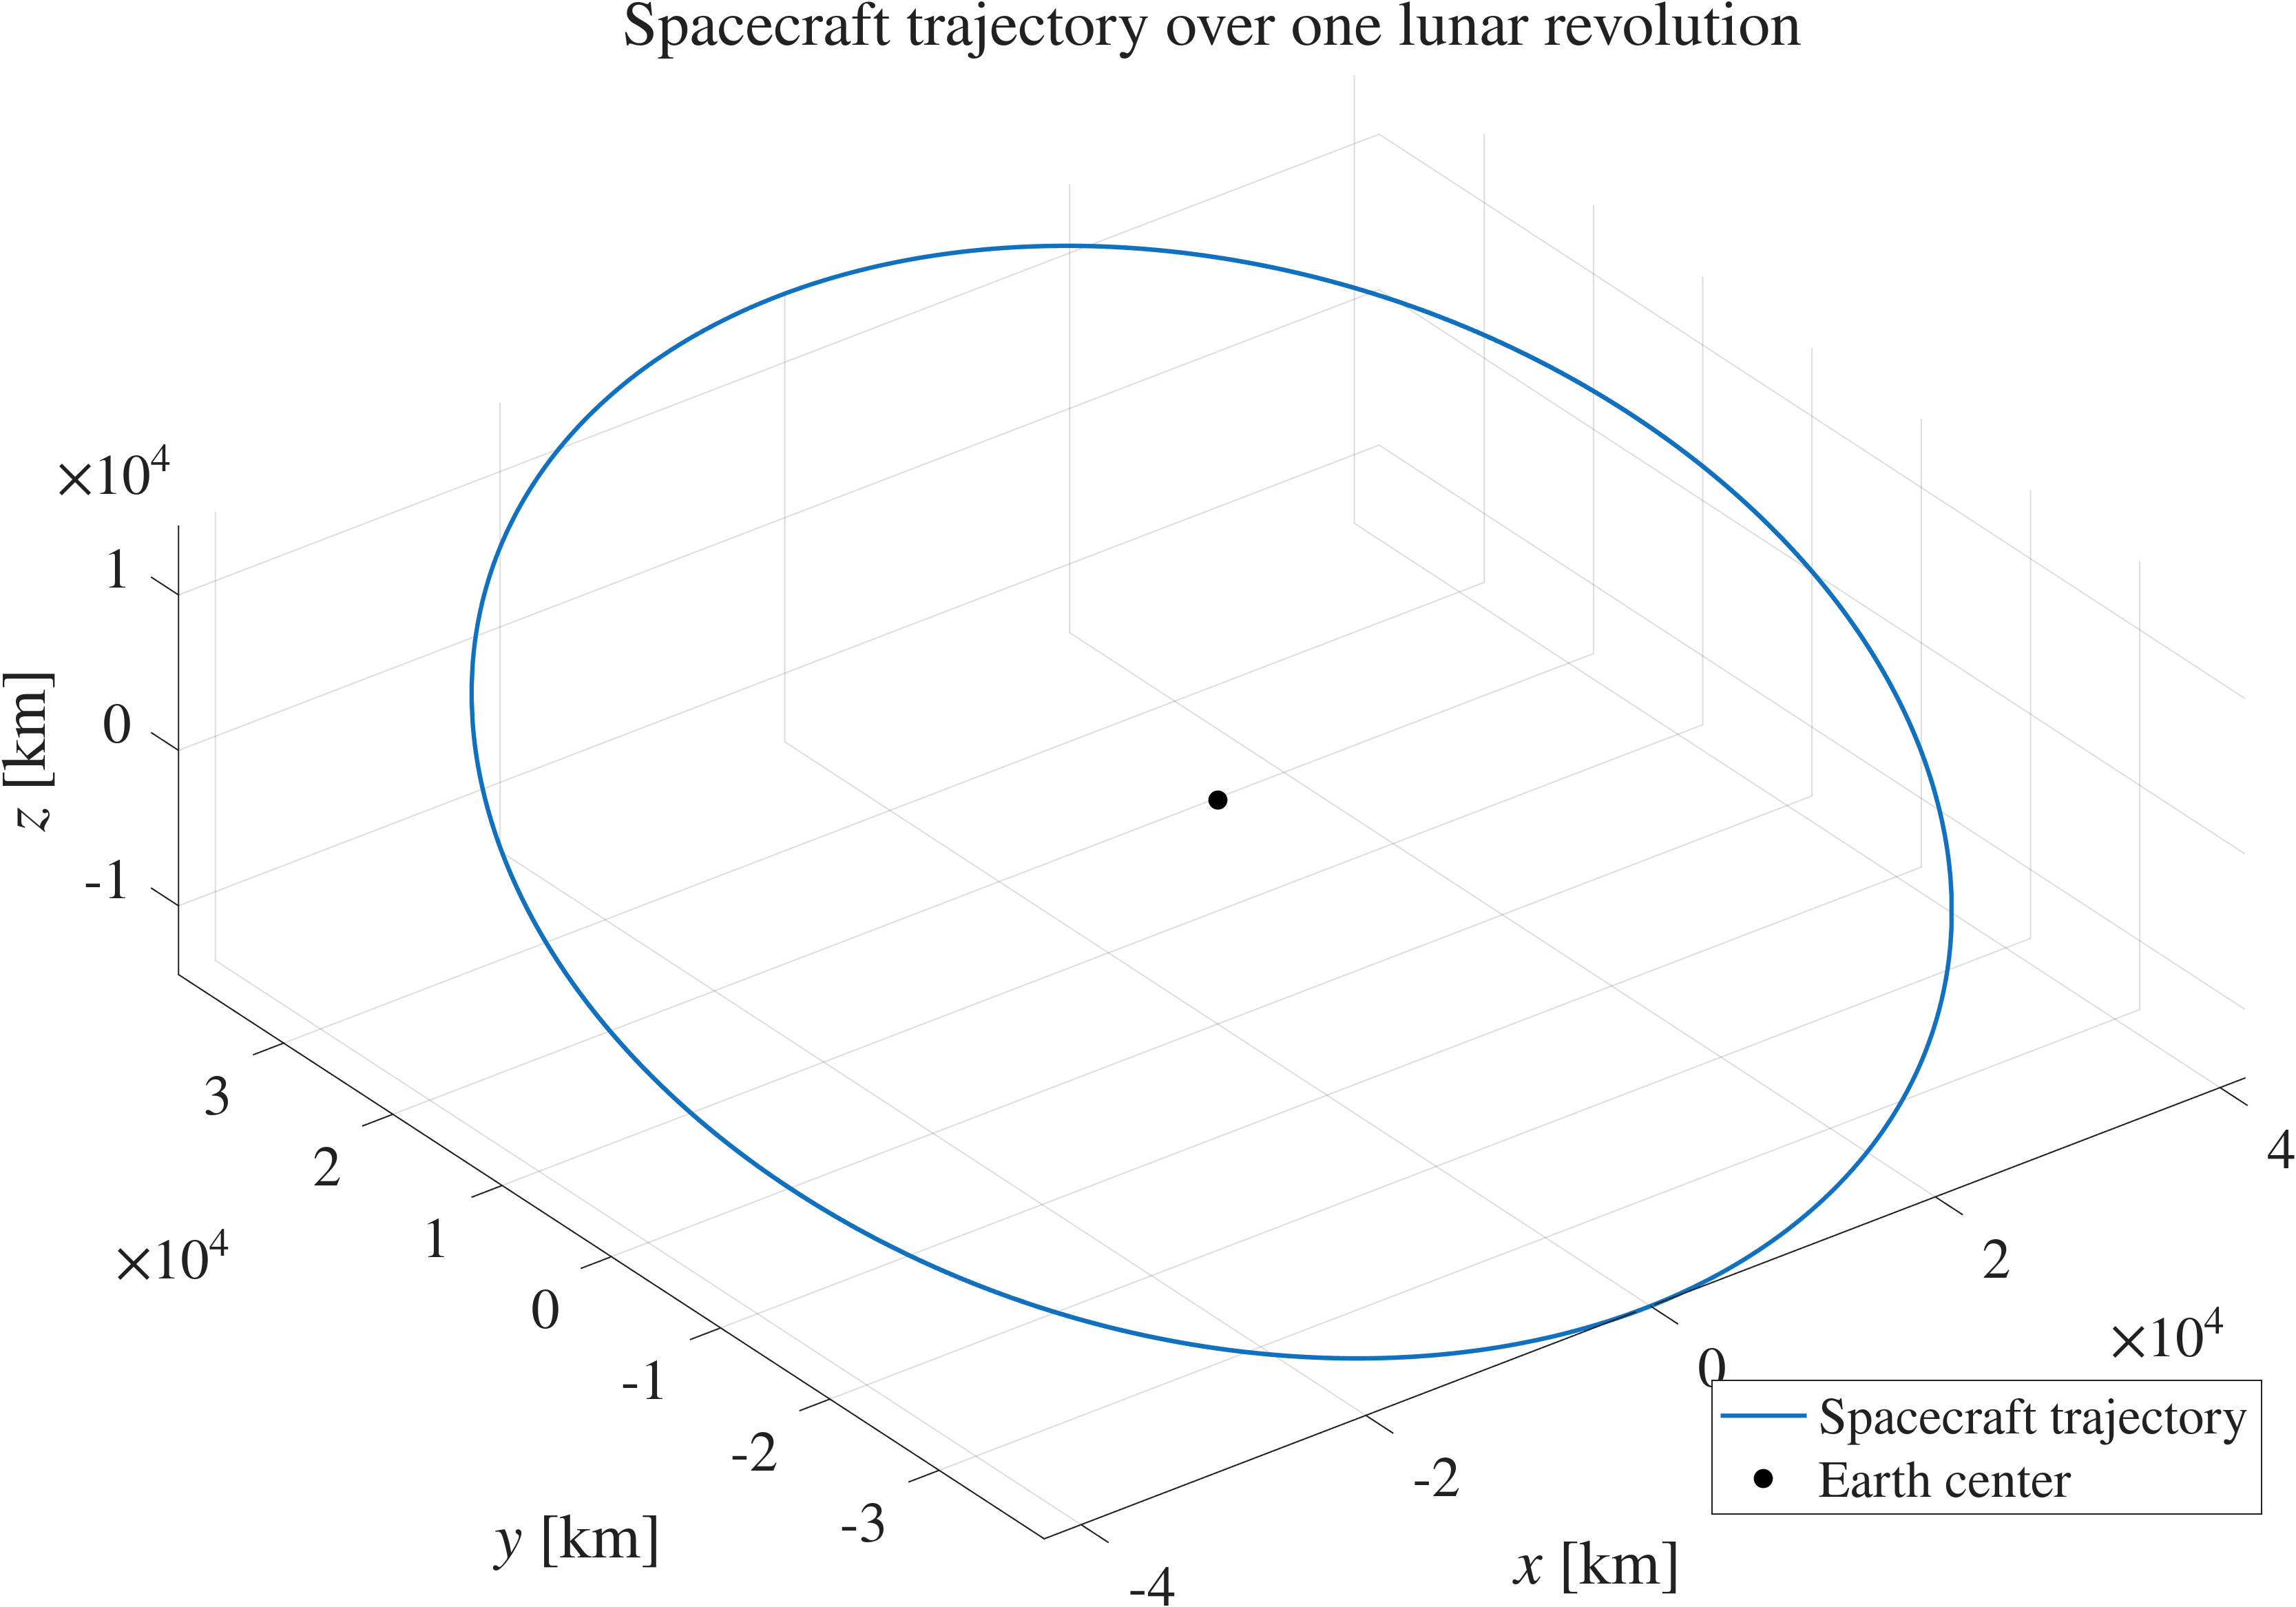
\includegraphics[width=\textwidth]{b3_trajectory_3d.png}
		\caption{3D view}
		\label{fig:b3_traj_3d}
	\end{subfigure}
	\hfill
	\begin{subfigure}{0.48\textwidth}
		\centering
		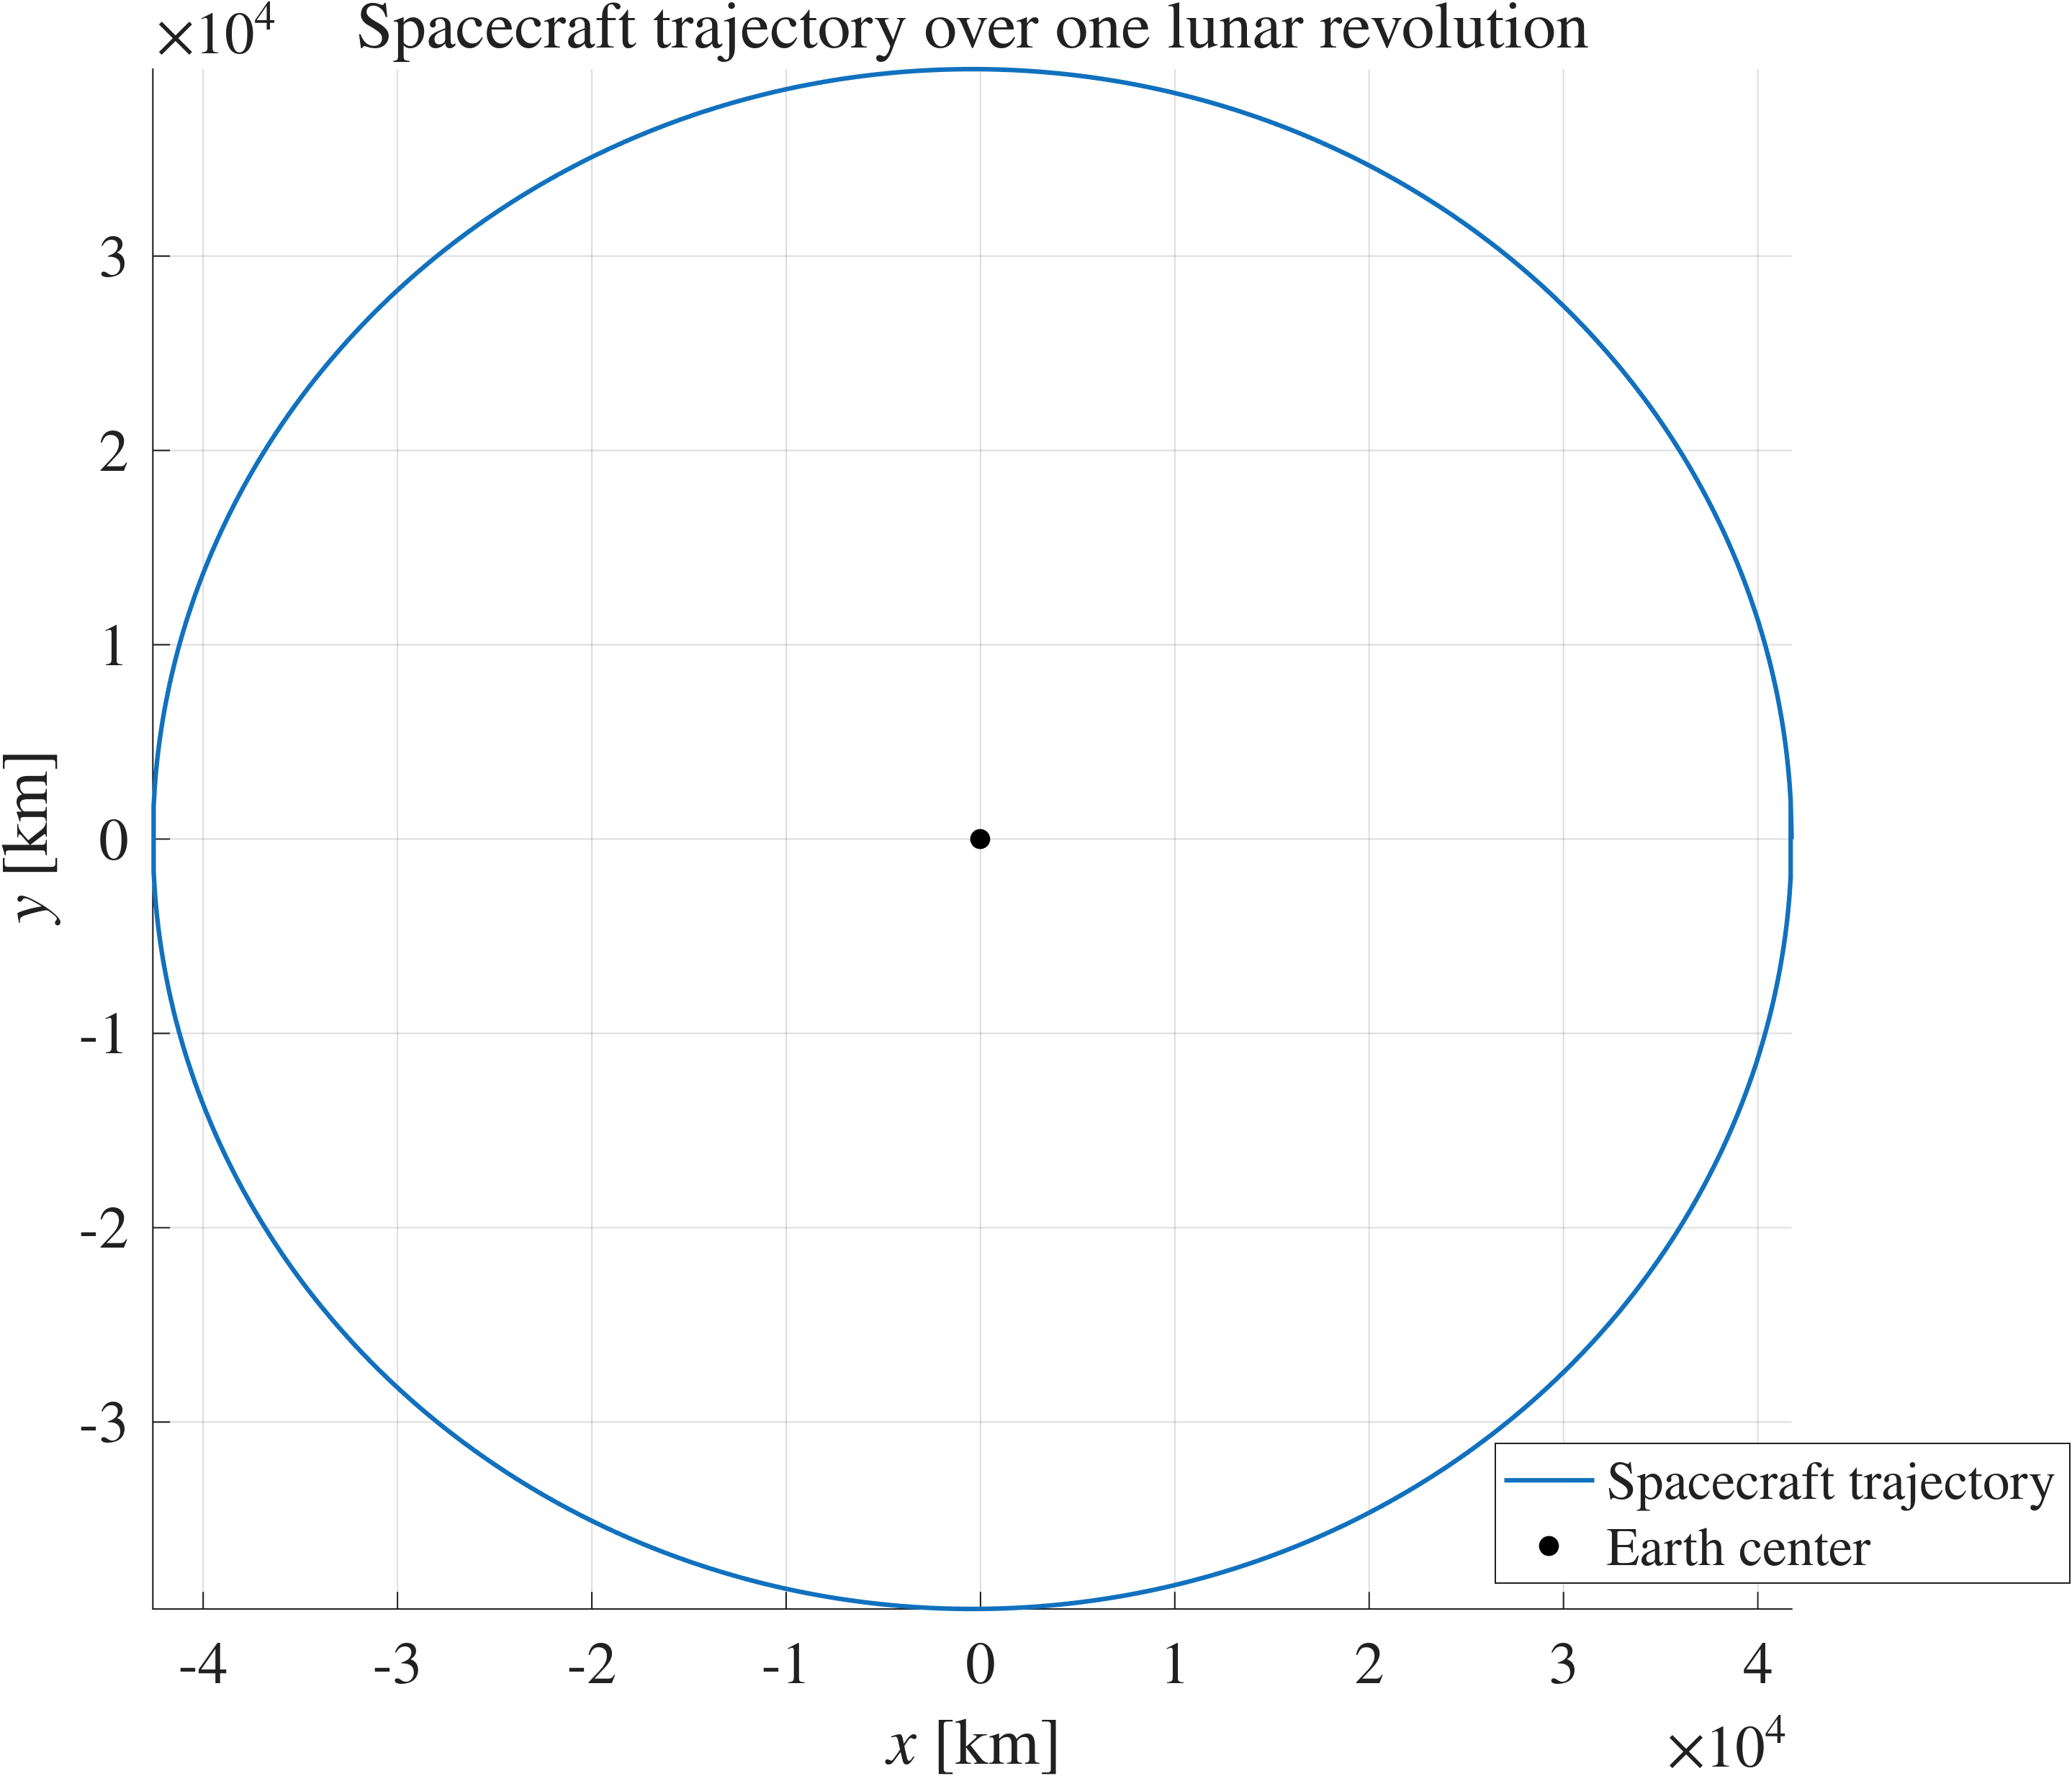
\includegraphics[width=\textwidth]{b3_trajectory_topdown.png}
		\caption{Top-down view ($x$-$y$ plane)}
		\label{fig:b3_traj_topdown}
	\end{subfigure}
	
	\begin{subfigure}{0.48\textwidth}
		\centering
		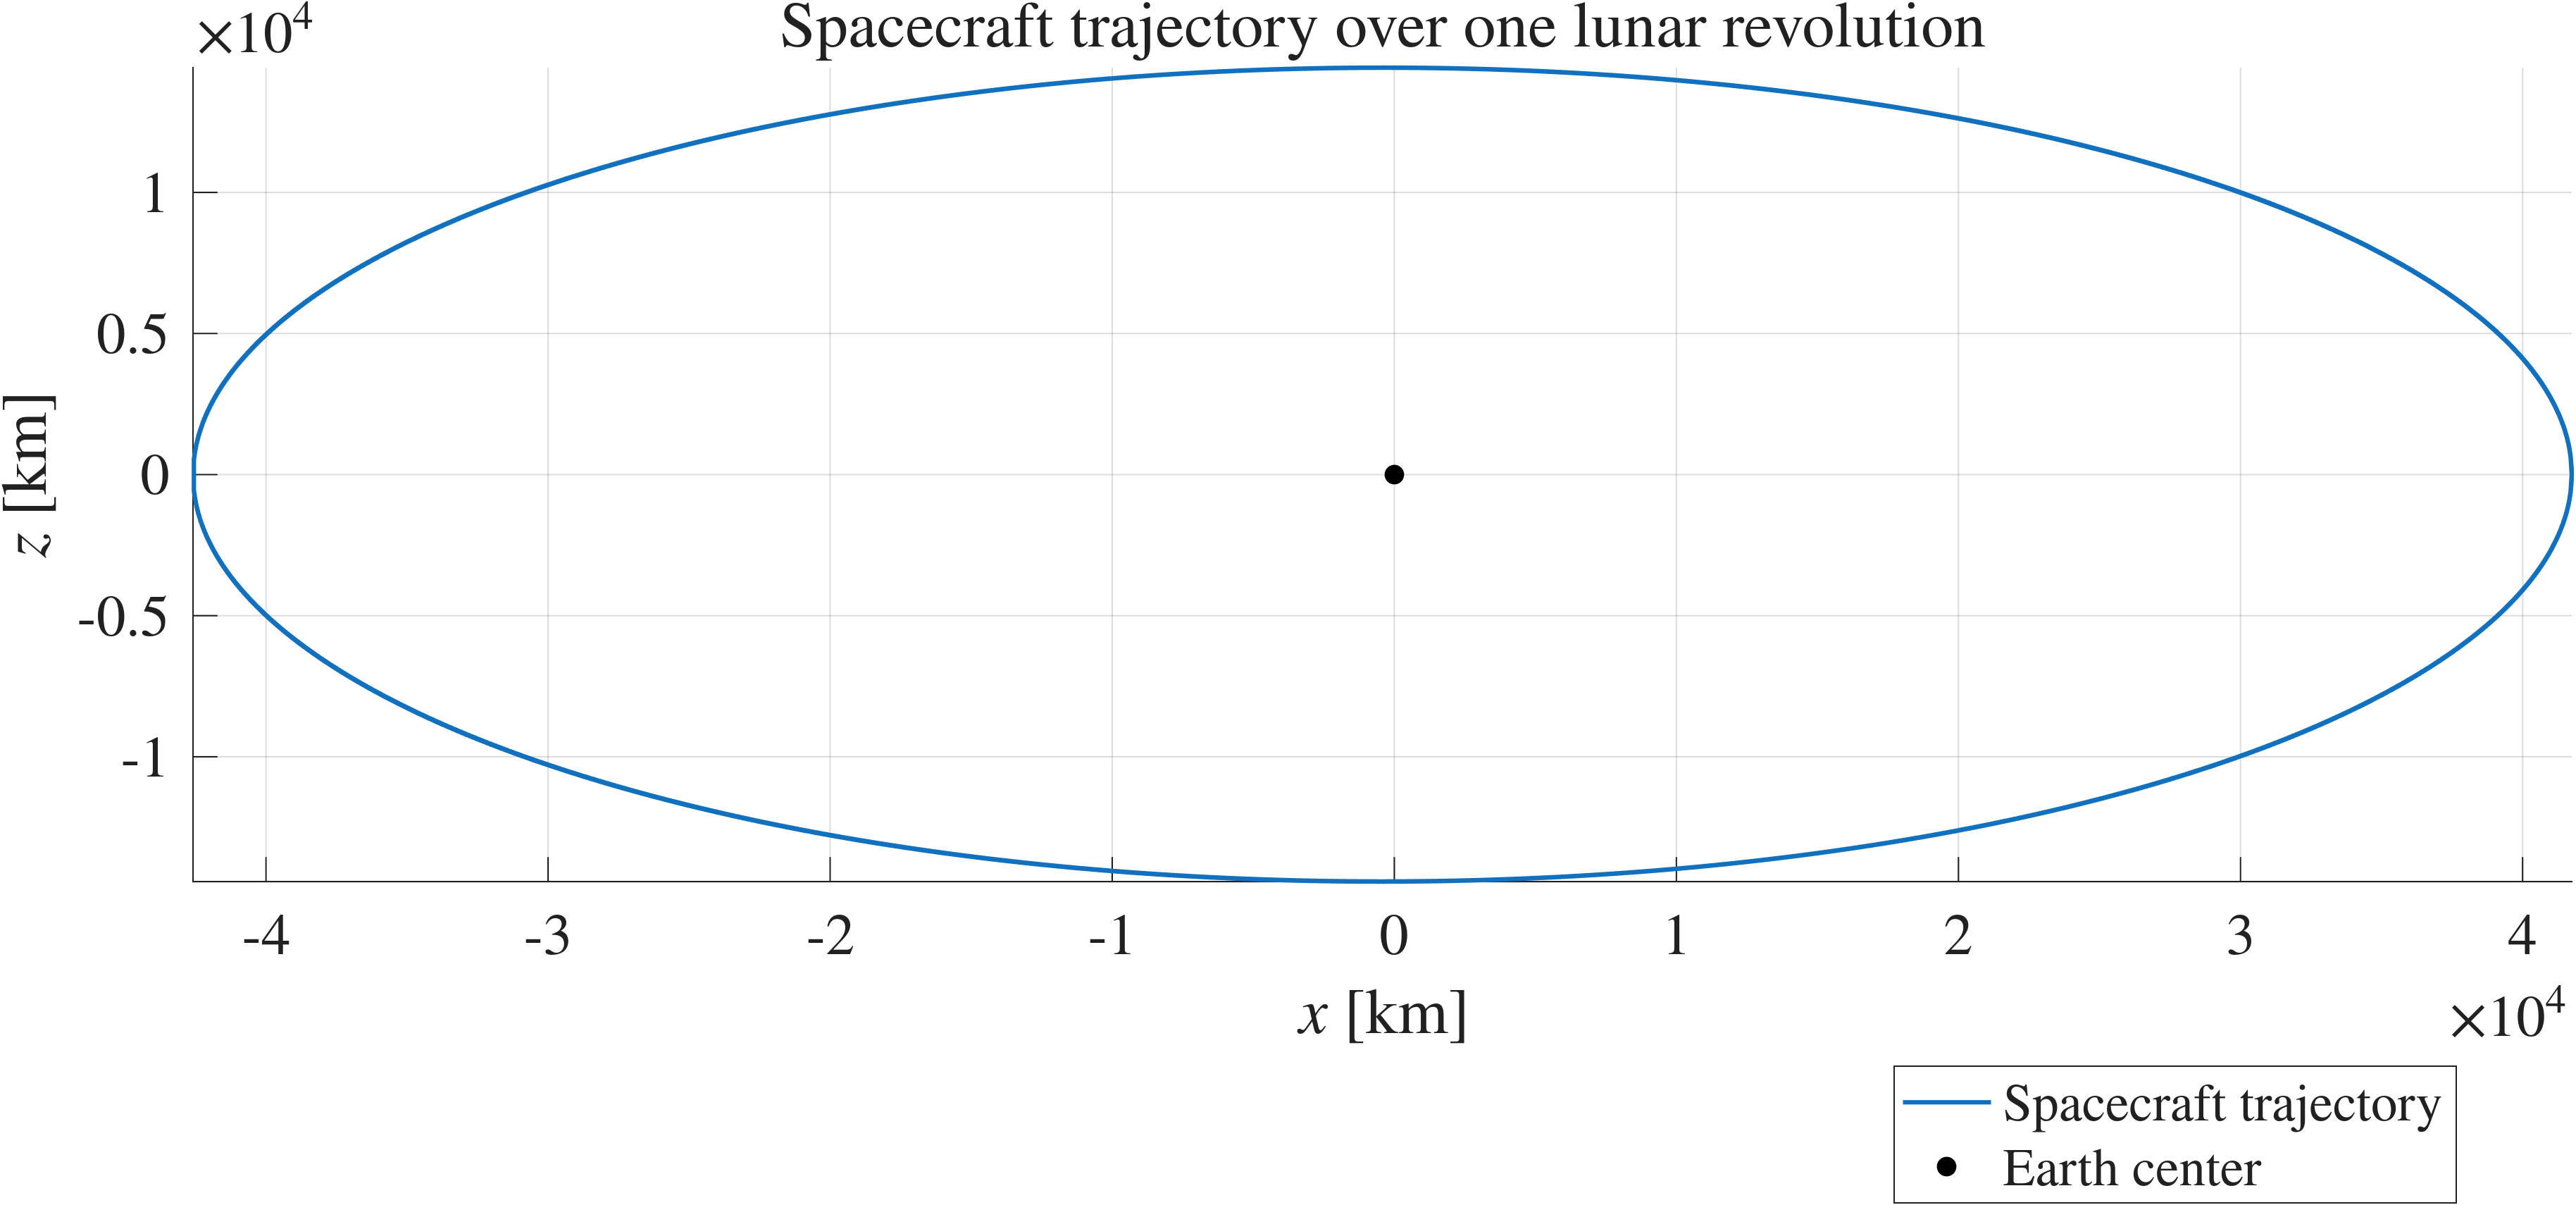
\includegraphics[width=\textwidth]{b3_trajectory_edgeon_xz.png}
		\caption{Edge-on view ($x$-$z$ plane)}
		\label{fig:b3_traj_edgeon_xz}
	\end{subfigure}
	\hfill
	\begin{subfigure}{0.48\textwidth}
		\centering
		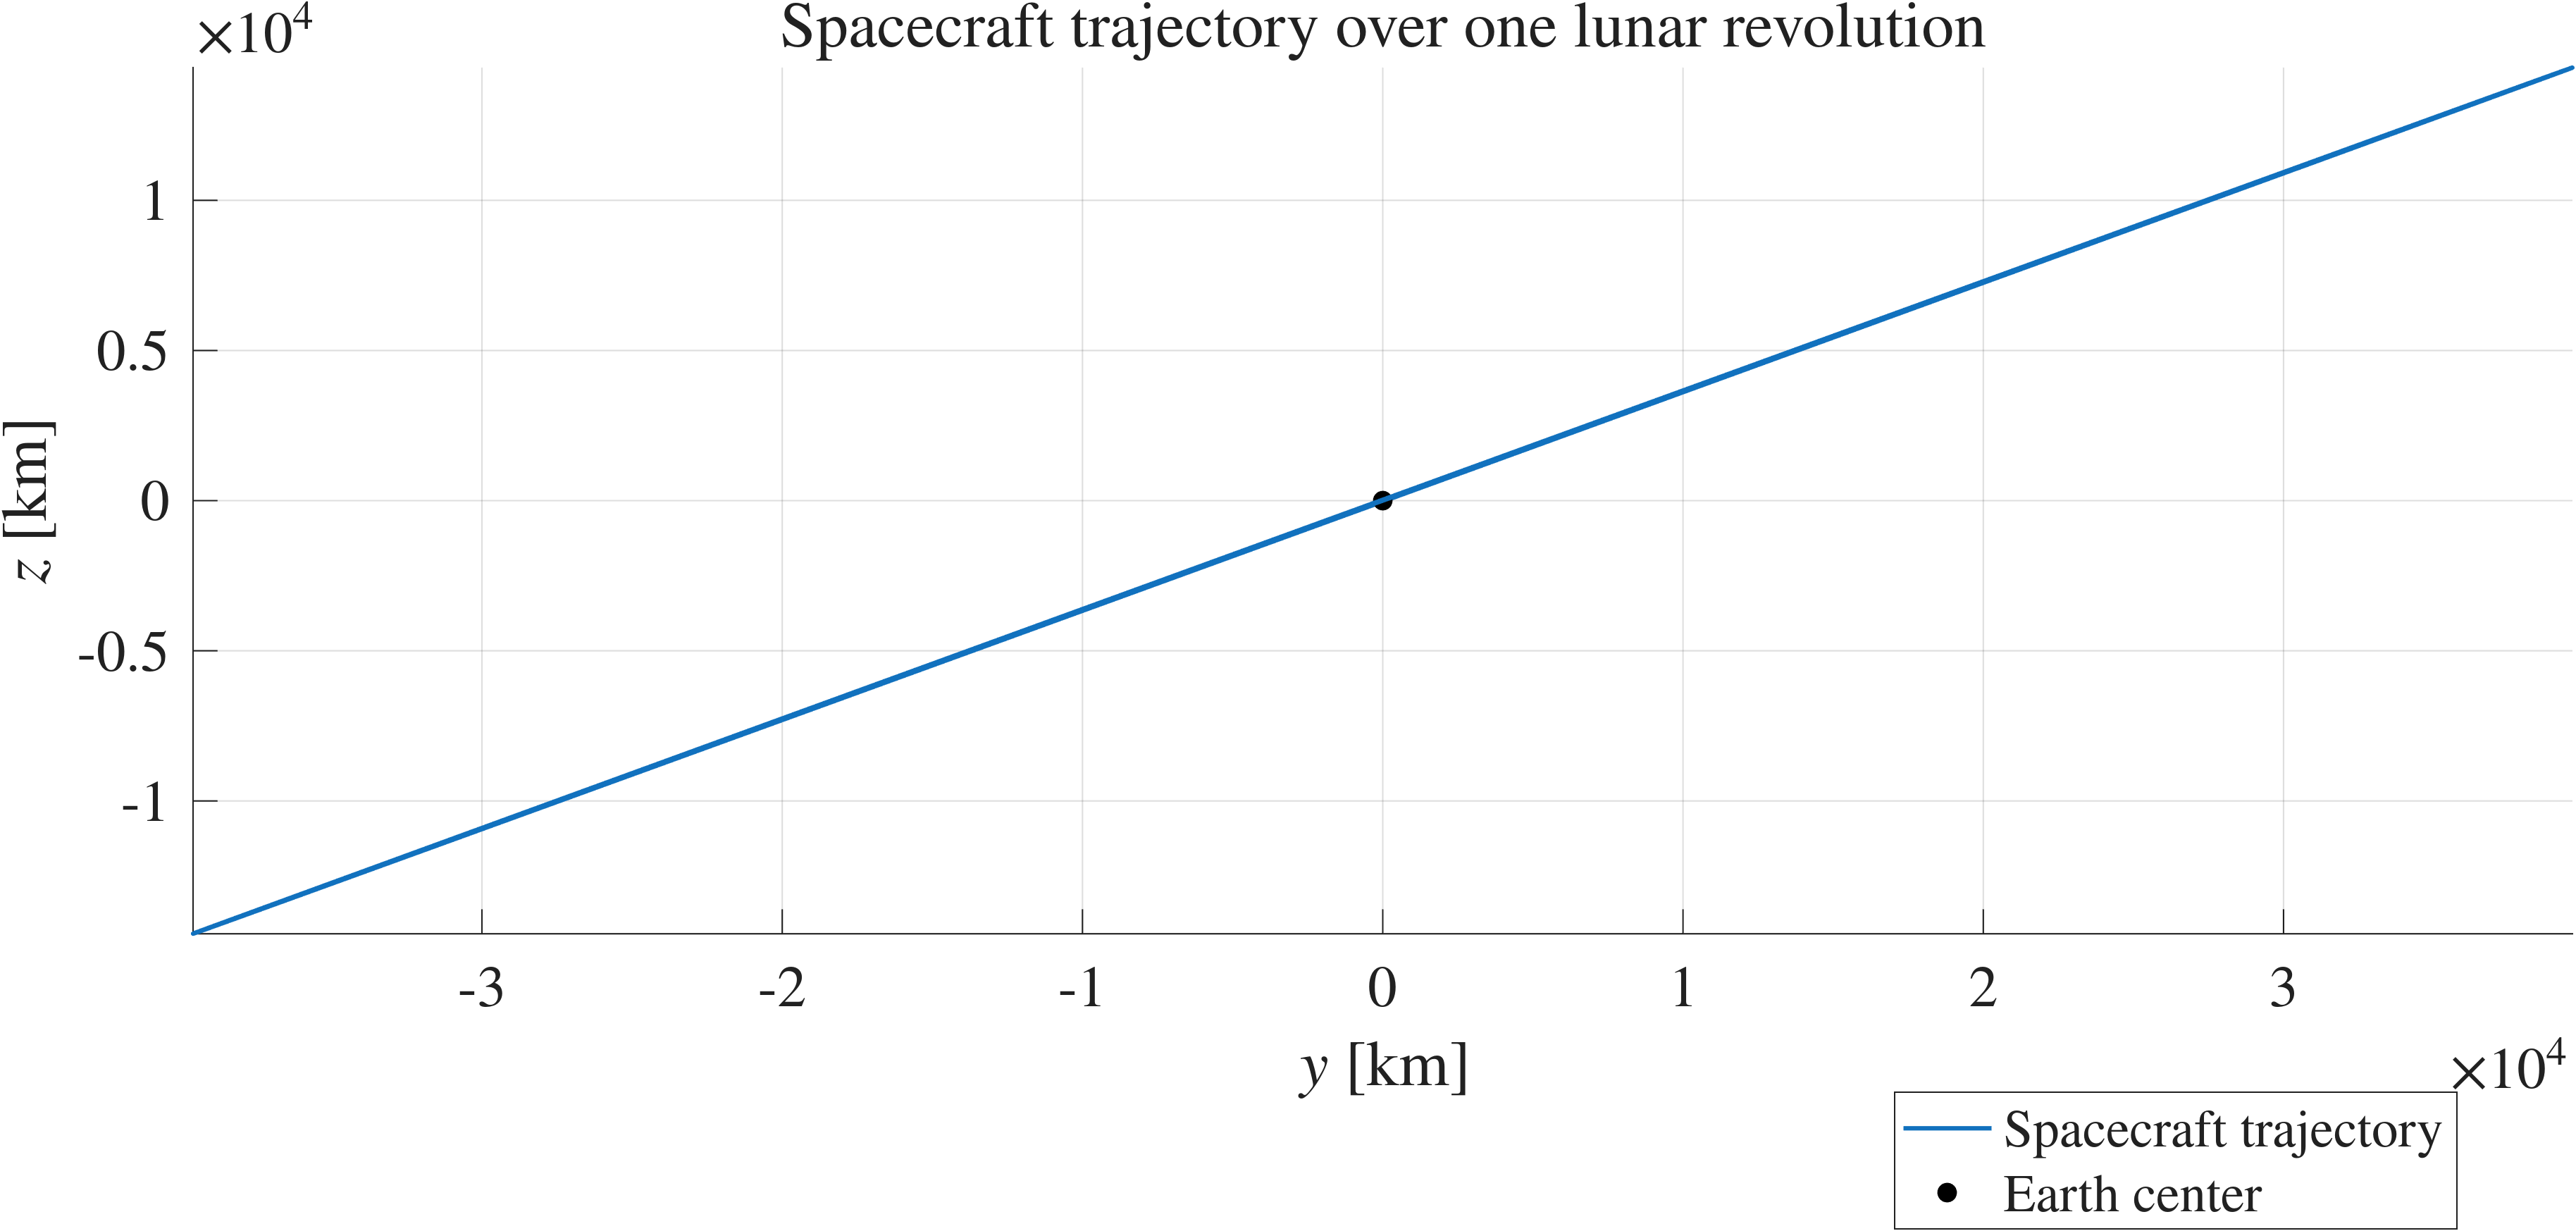
\includegraphics[width=\textwidth]{b3_trajectory_edgeon_yz.png}
		\caption{Edge-on view ($y$-$z$ plane)}
		\label{fig:b3_traj_edgeon_yz}
	\end{subfigure}
	\caption{Spacecraft trajectory in configuration space over one lunar revolution.}
	\label{fig:b3_trajectory}
\end{figure}

\newpage

Plot of the time history of $\boldsymbol{q}$ coordinates:
\begin{figure}[H]
	\centering
	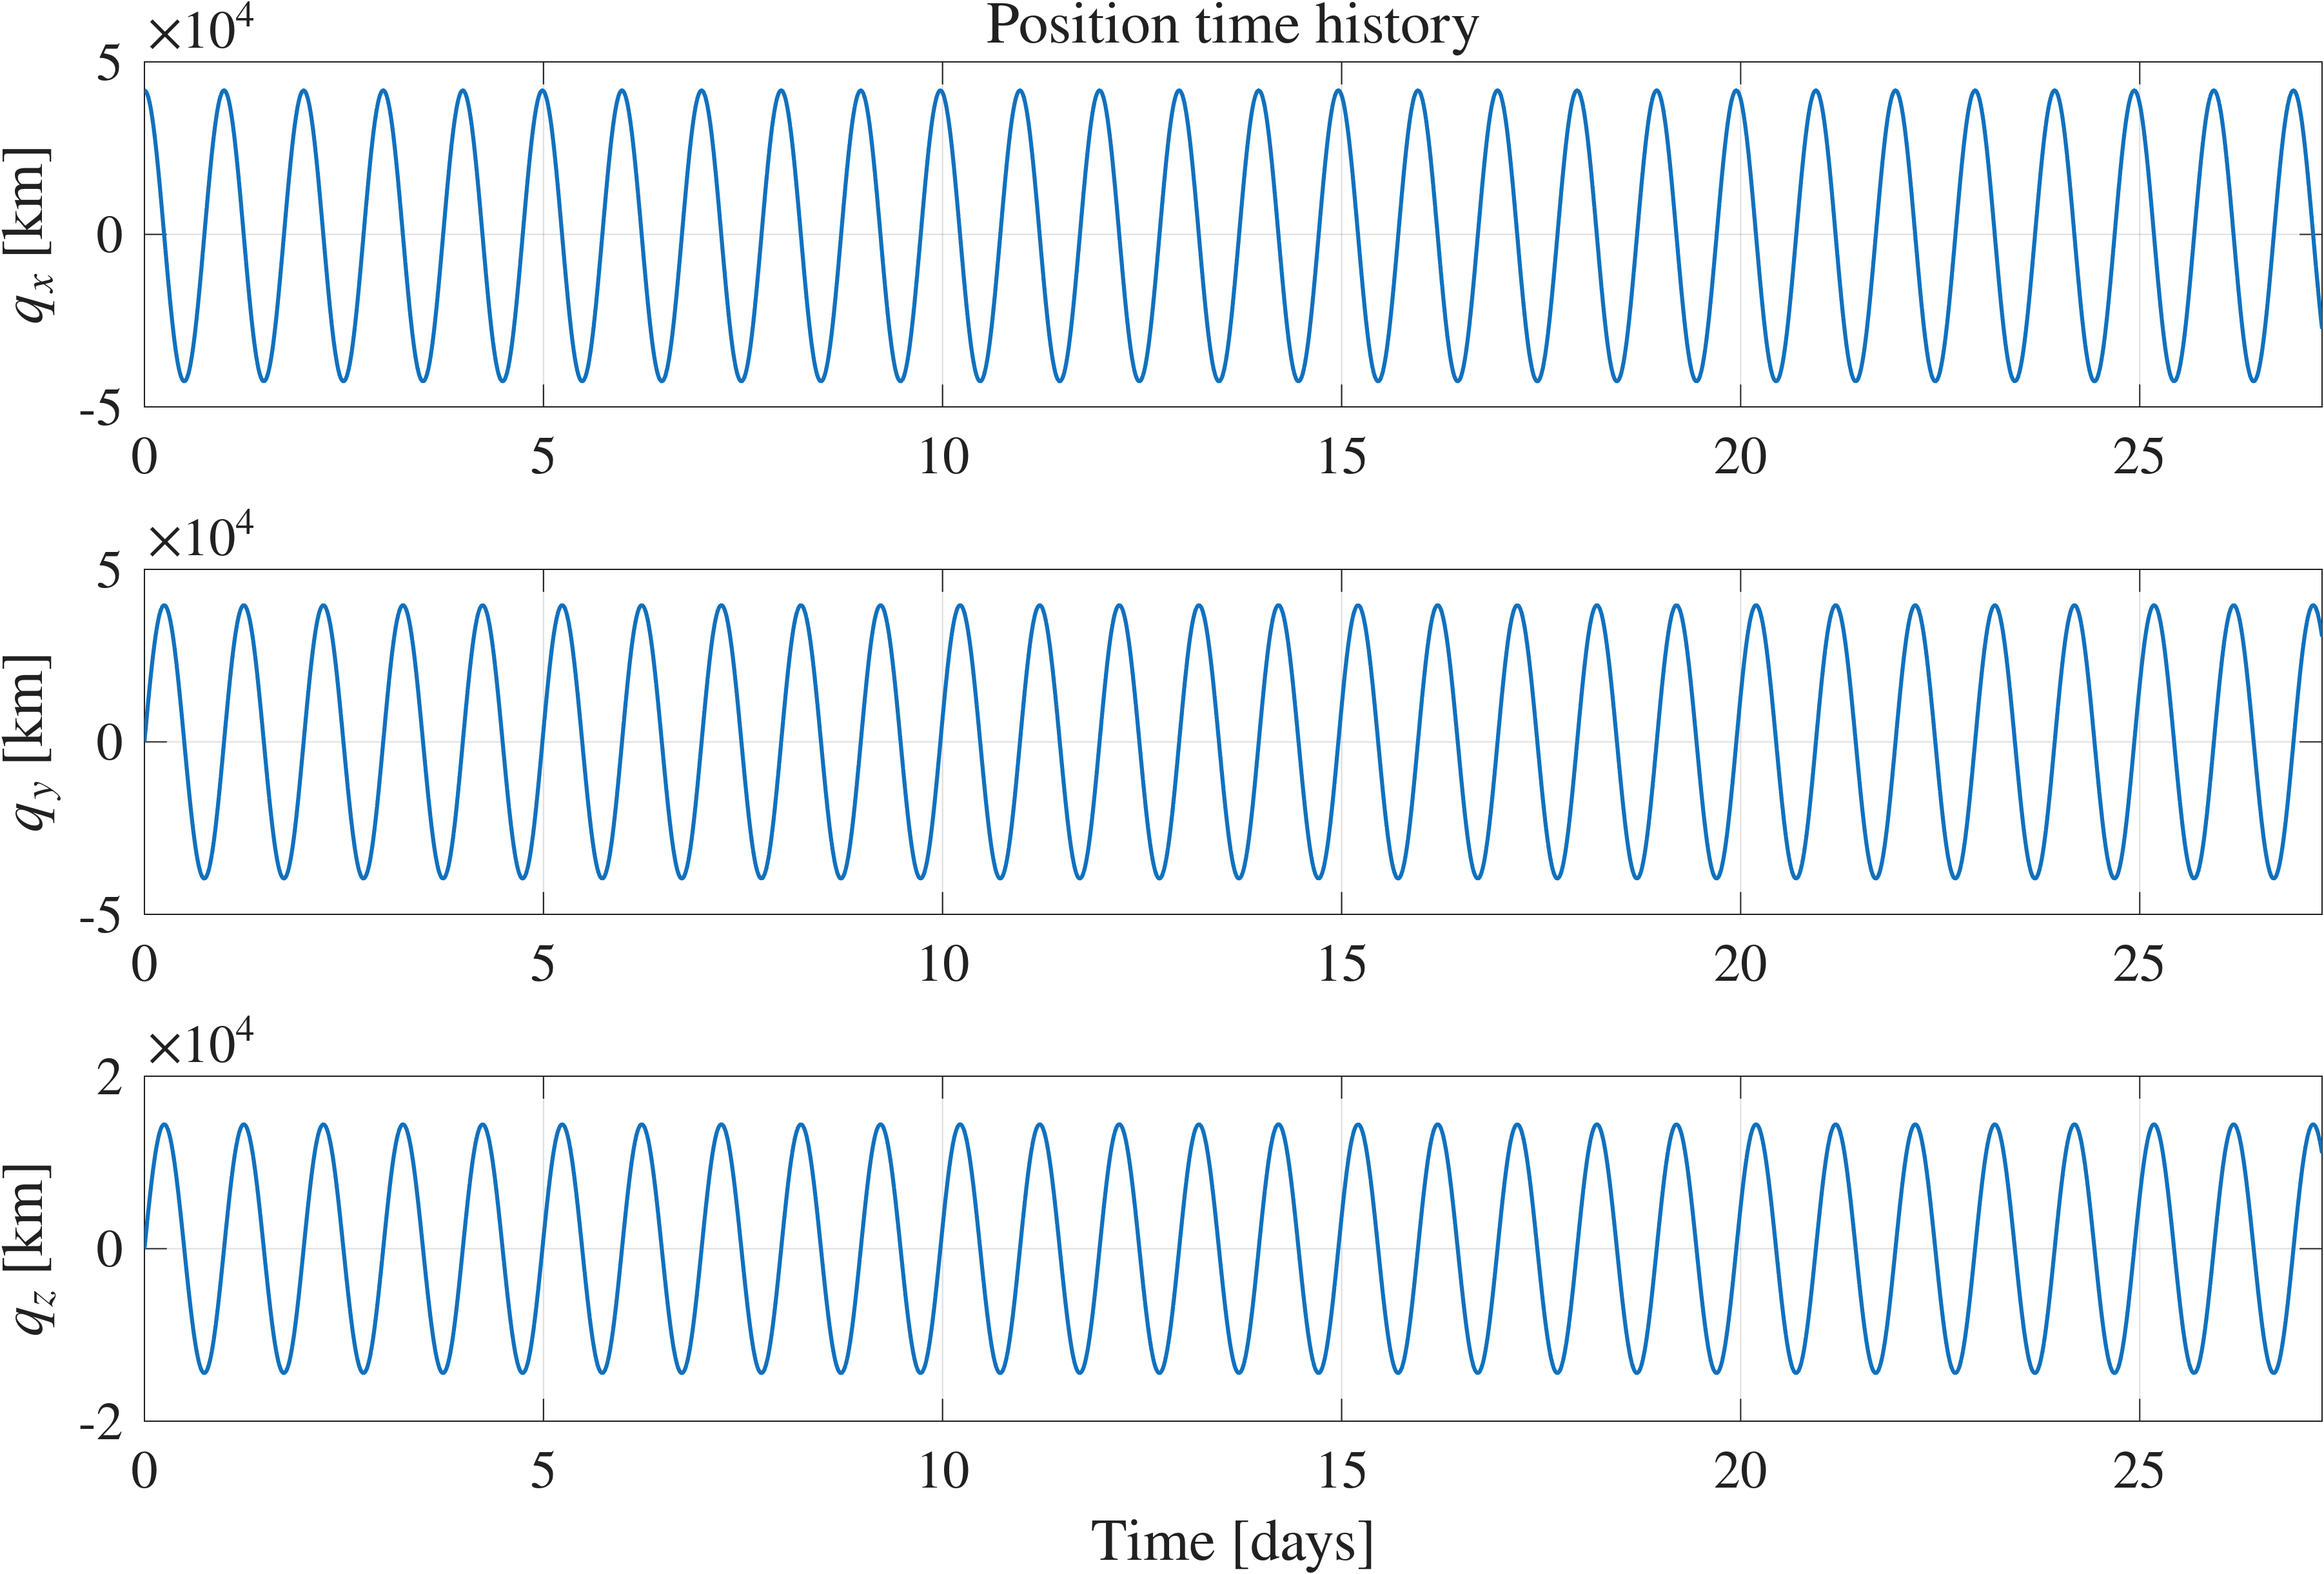
\includegraphics[width=0.9\textwidth]{b3_q.png}
	\caption{Position $\boldsymbol{q}(t)$ components over one lunar revolution.}
	\label{fig:b3_q}
\end{figure}

And time history plot of their conjugate momenta $\boldsymbol{p}$:
\begin{figure}[H]
	\centering
	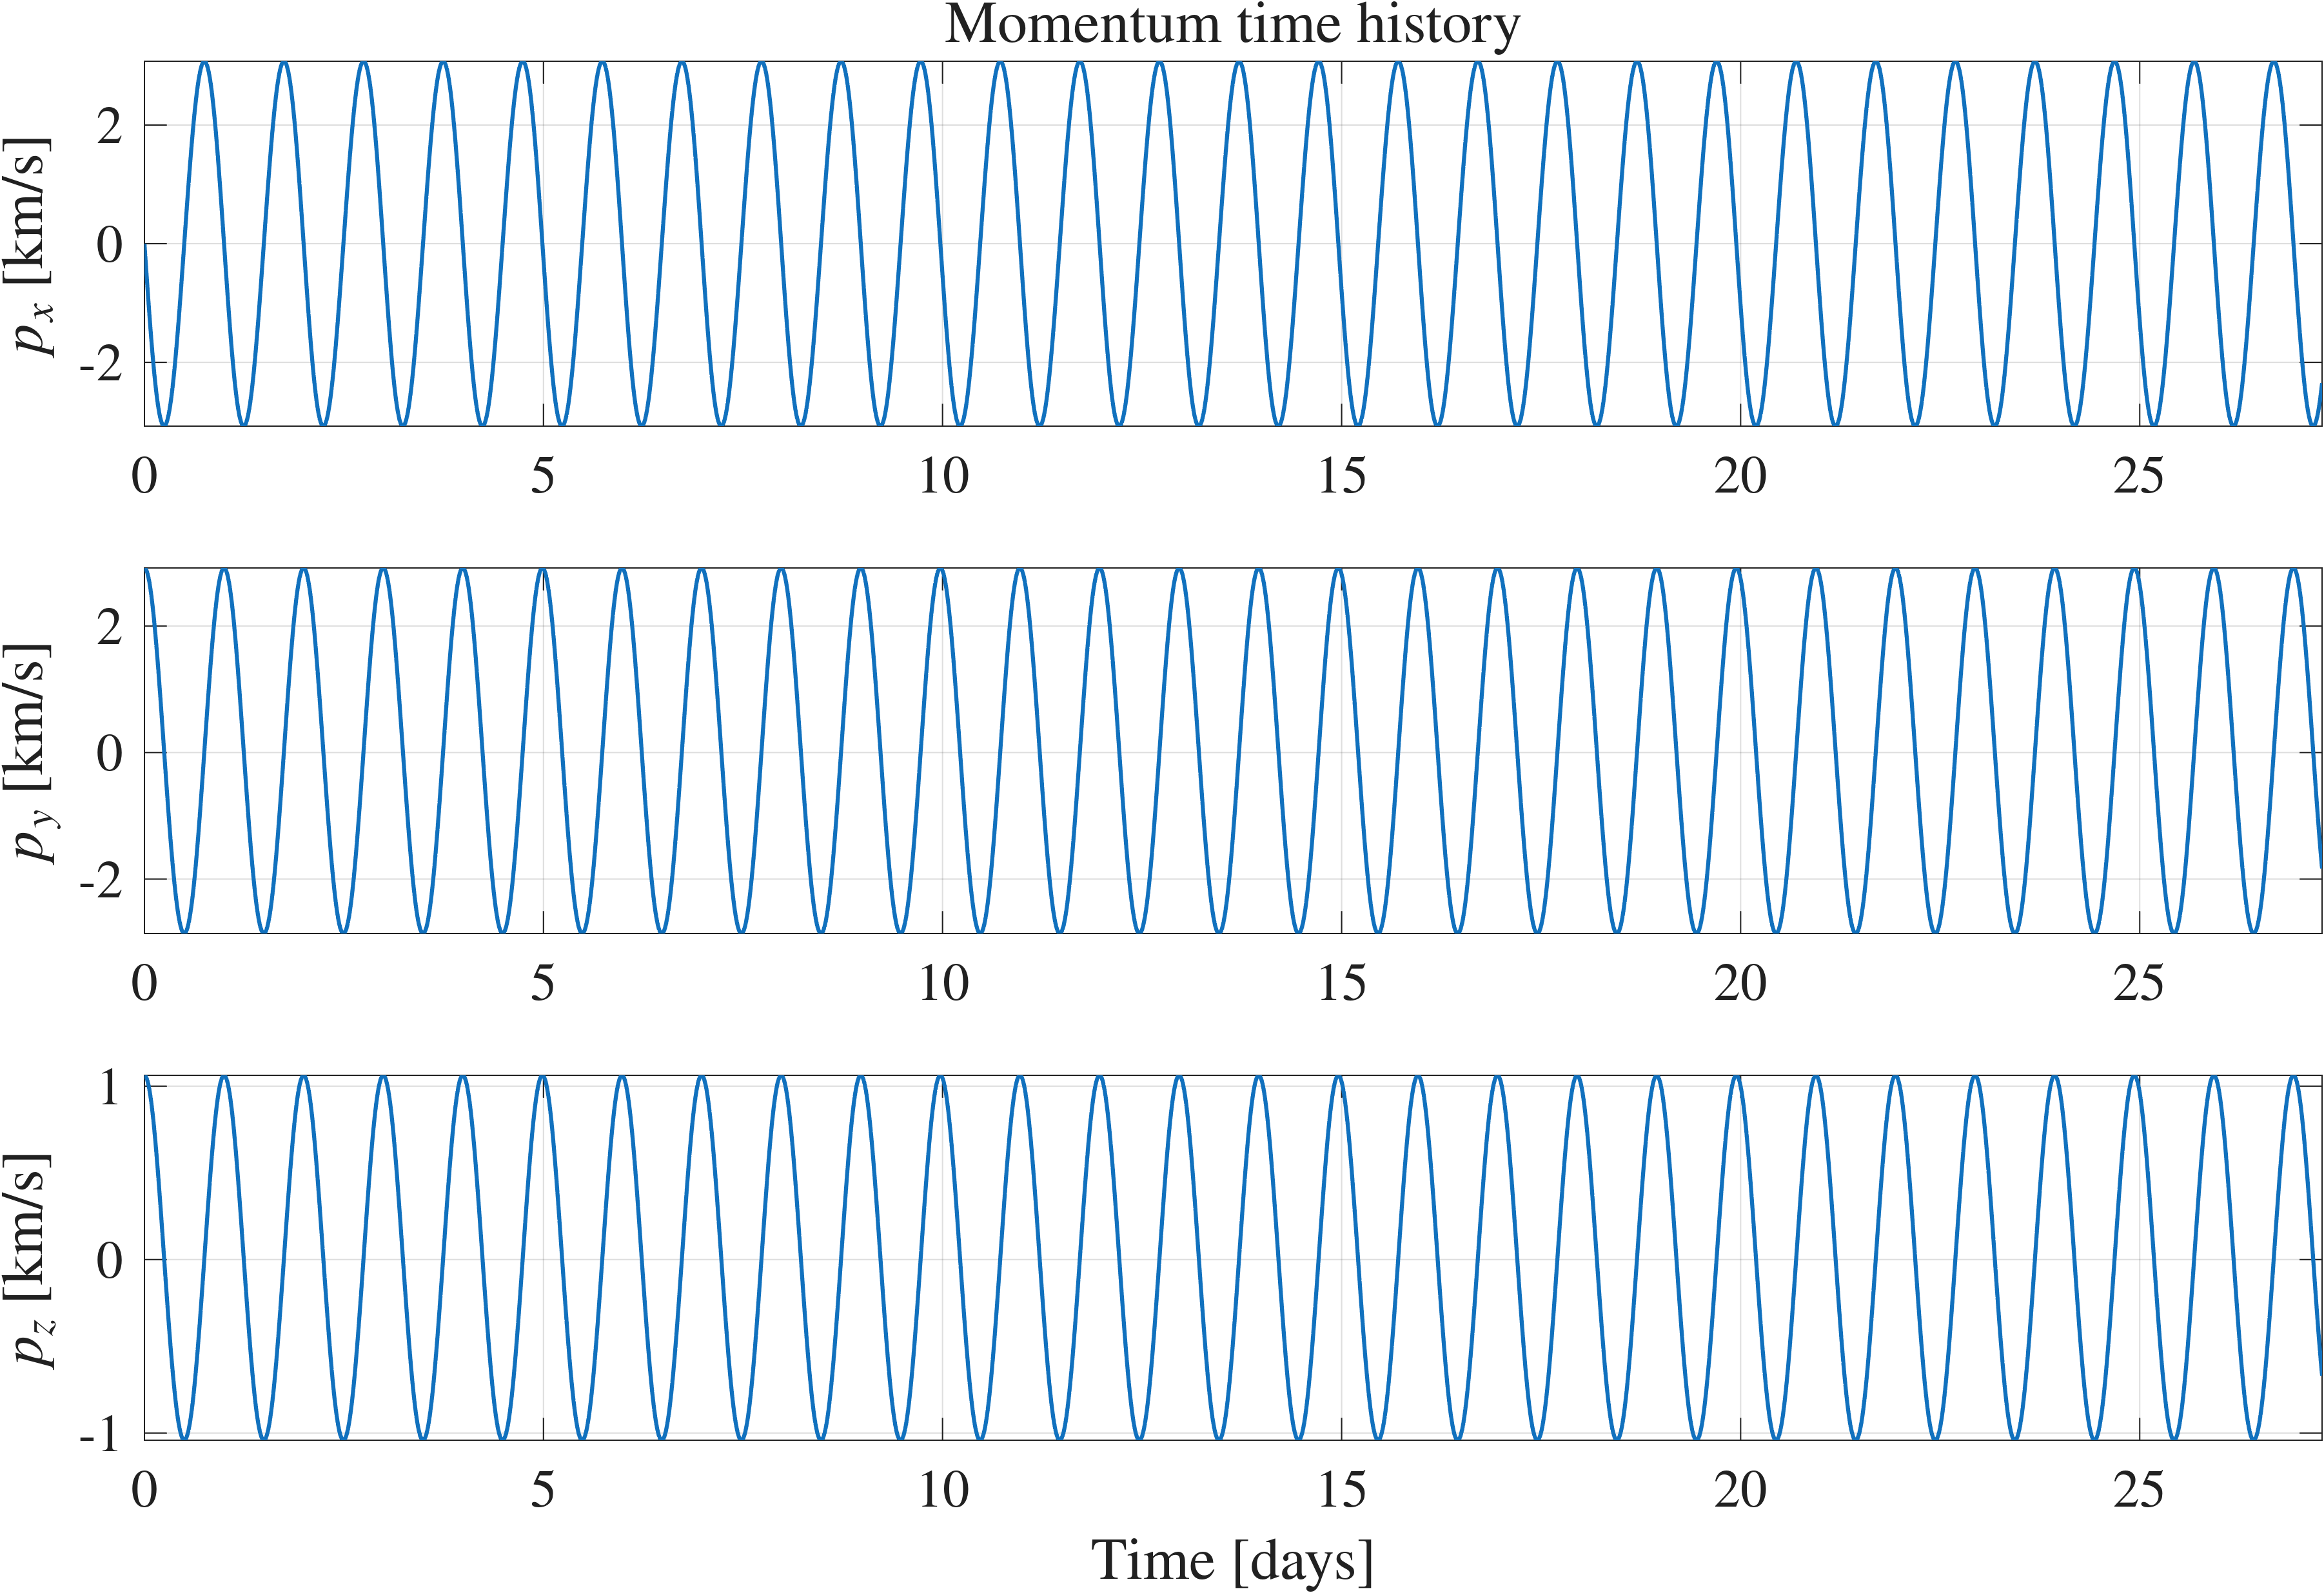
\includegraphics[width=0.9\textwidth]{b3_p.png}
	\caption{Momentum $\boldsymbol{p}(t)$ components over one lunar revolution.}
	\label{fig:b3_p}
\end{figure}

The variation of the Hamiltonian $H$ from its initial state $H(0)$:
\begin{figure}[H]
	\centering
	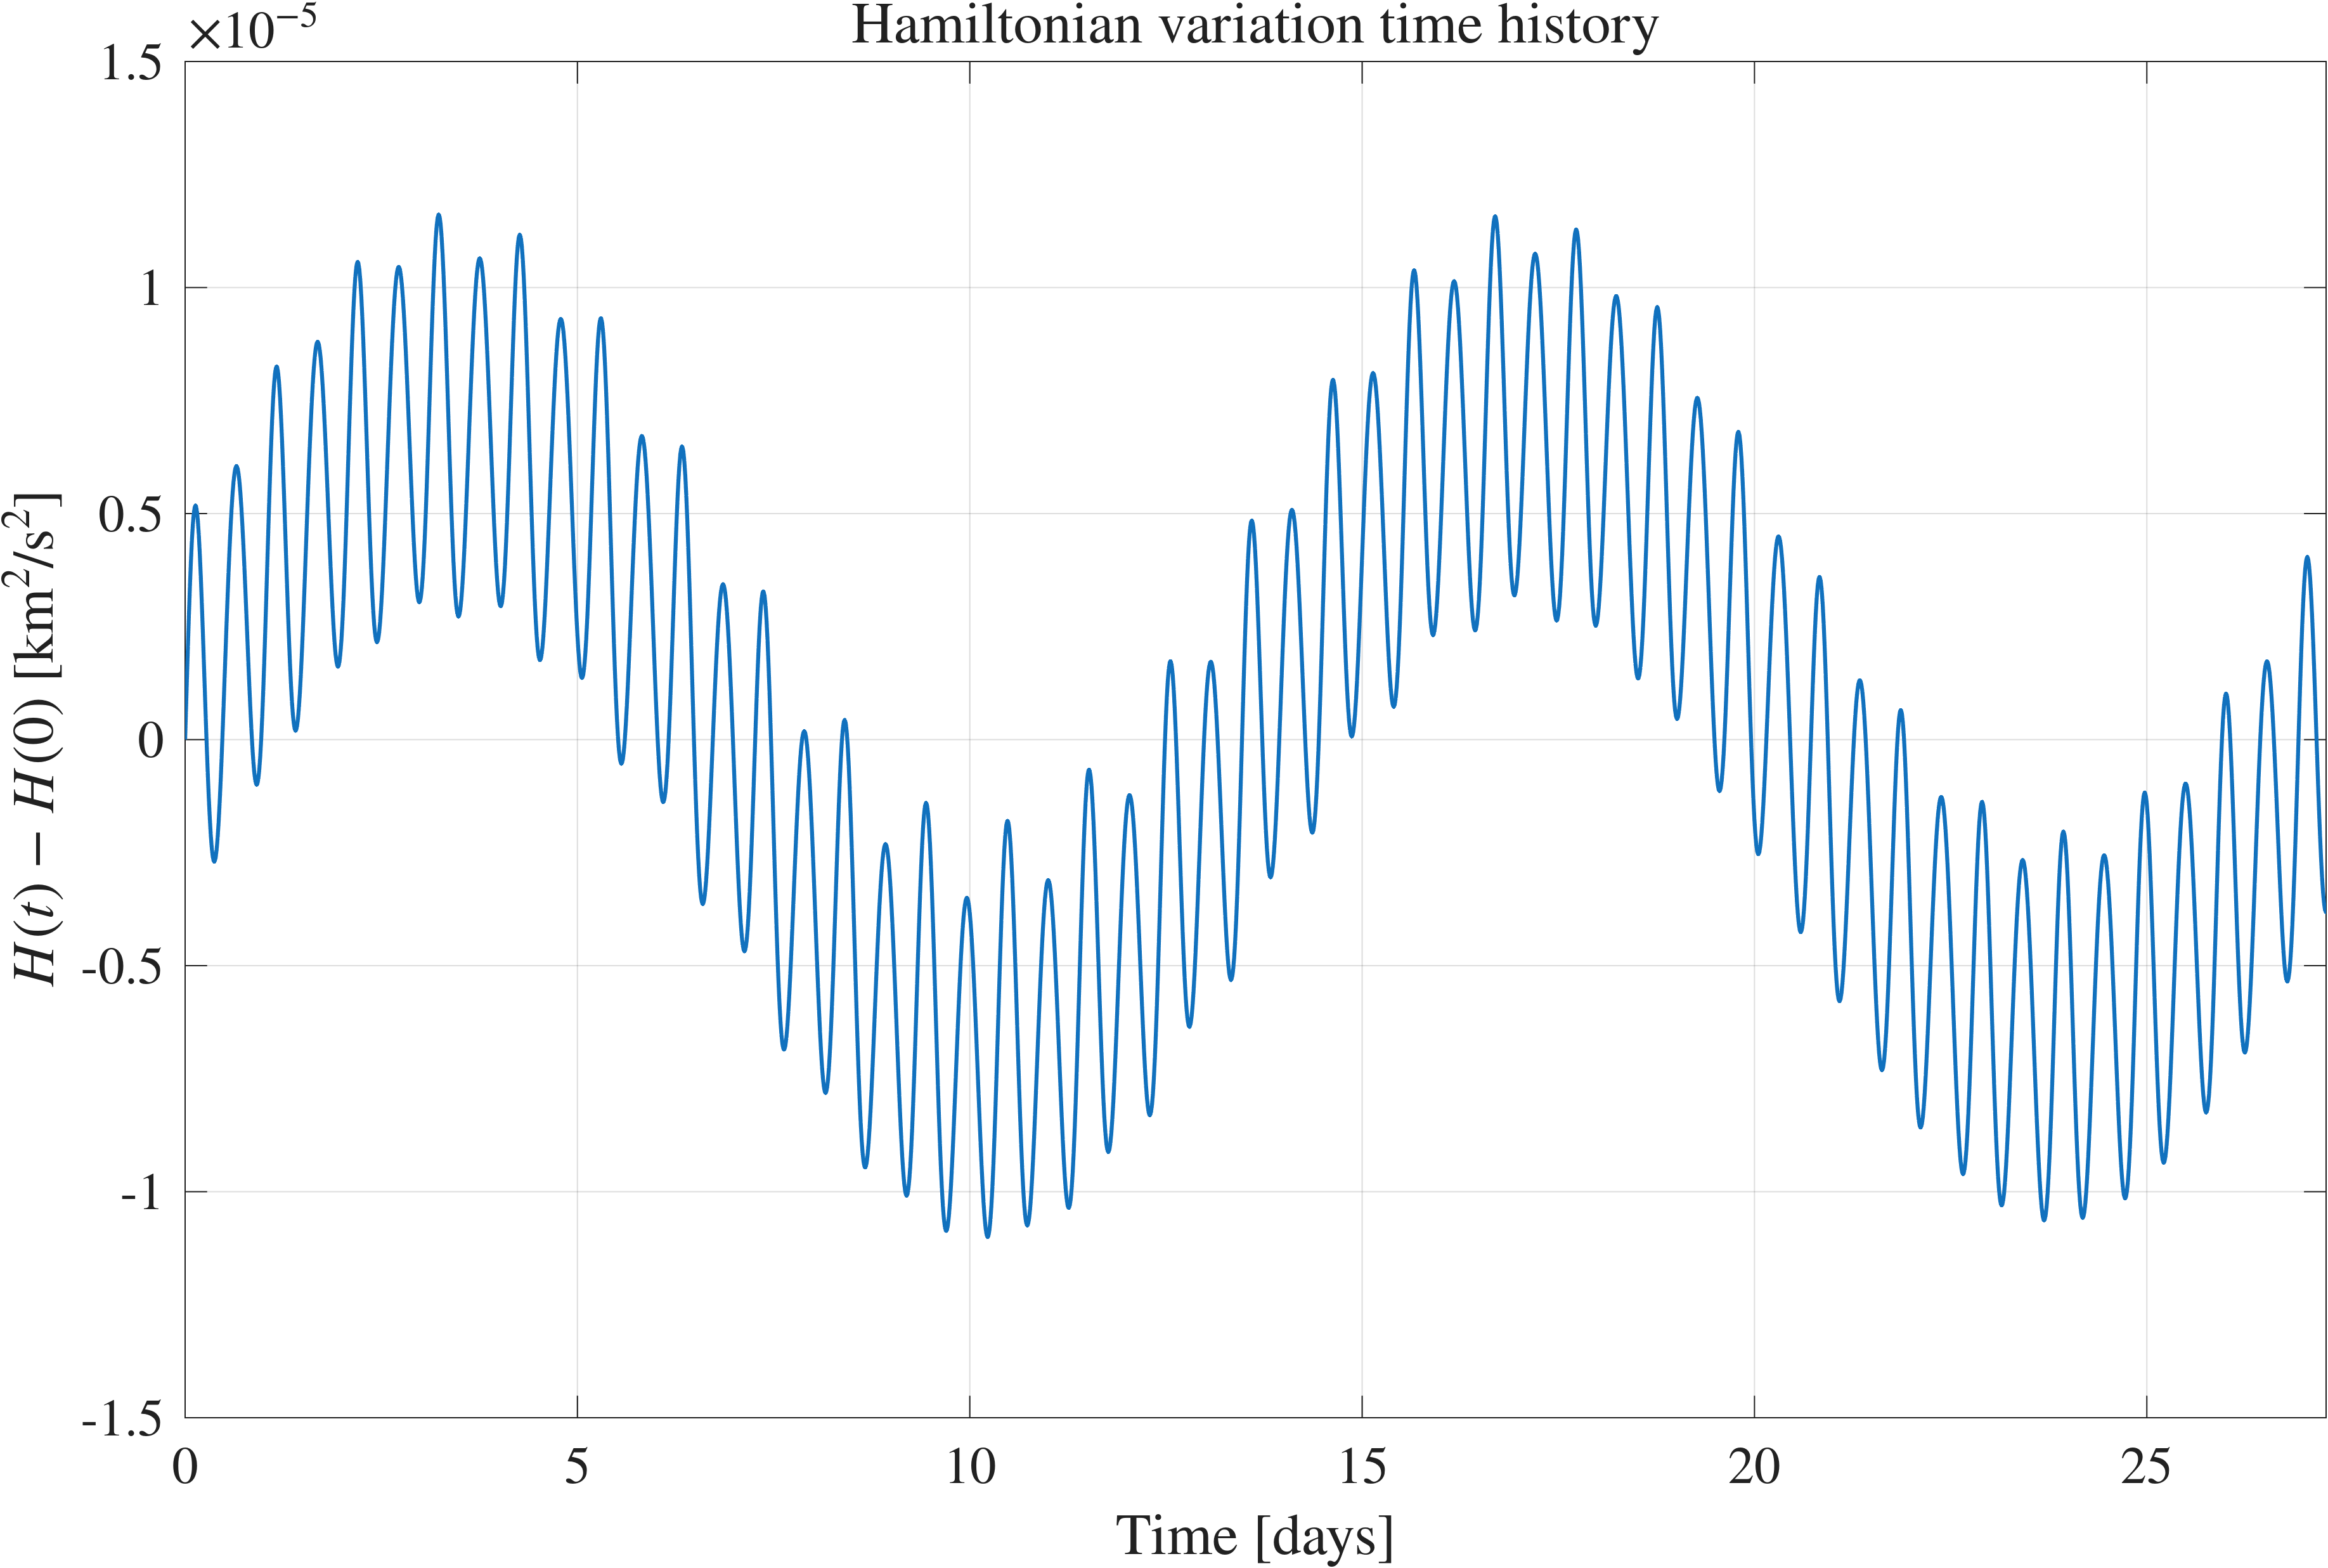
\includegraphics[width=0.9\textwidth]{b3_H.png}
	\caption{Hamiltonian variation $H(t)-H(0)$ over one lunar revolution.}
	\label{fig:b3_H}
\end{figure}

And the time history fo the extended Hamiltonian $\widehat{H}(t)$:
\begin{figure}[H]
	\centering
	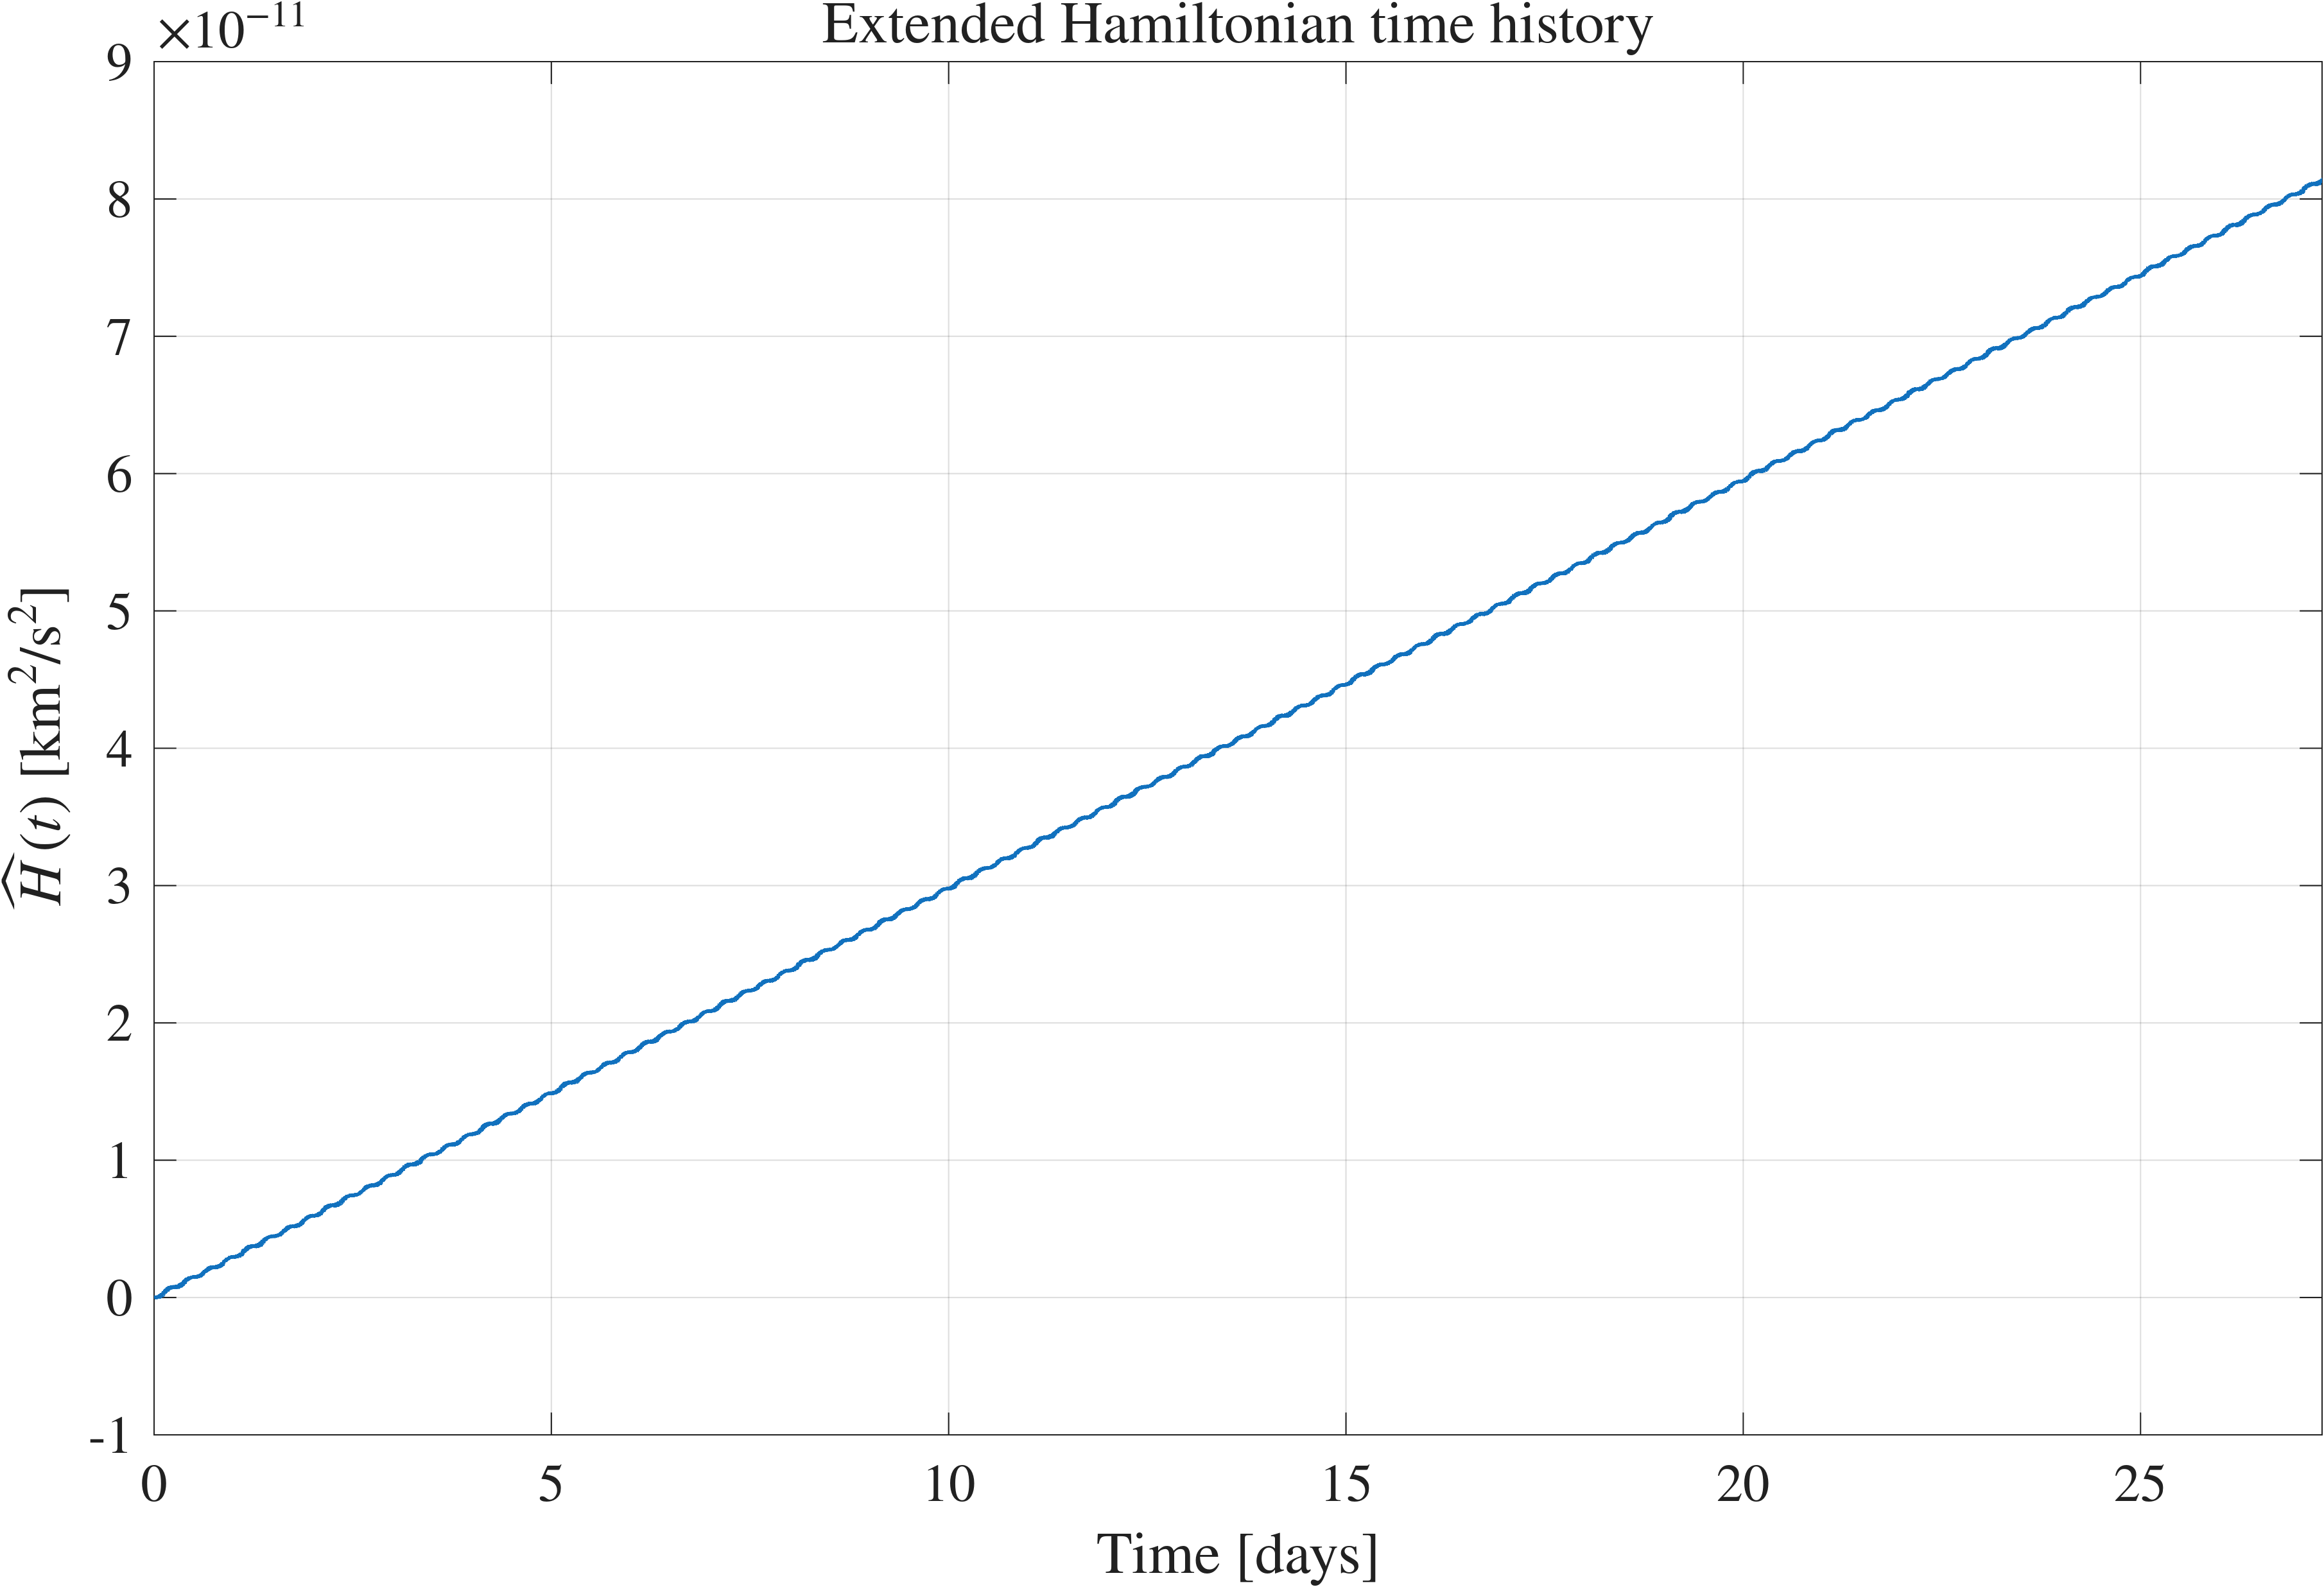
\includegraphics[width=0.9\textwidth]{b3_Hhat.png}
	\caption{Extended Hamiltonian $\widehat{H}(t)$ over one lunar revolution.}
	\label{fig:b3_Hhat}
\end{figure}

\newpage

\begin{mdframed}[linewidth=1pt, innertopmargin=10pt, innerbottommargin=10pt]
	From the above plots we see that the spacecraft successfully maintains a nearly circular orbit about the Earth at what appears to be the correct inclination. \\
	
	From the time history plots of $\boldsymbol{q}$ and $\boldsymbol{p}$, we see that all coordinates repeat the same oscillation completely $27$ times with different amplitudes proportional to their expected contributions to the angled orbit, and a partial oscillation past the $27$th one. This would suggest that the spacecraft orbited the Earth $27$ times within that period and started a $28$th orbit. We know the expected orbital period of the spacecraft's two-body orbit around the Earth for the given initial conditions was:
	\begin{equation}
		\begin{split}
			T&=2\pi\sqrt{\frac{a^3}{\mu}}=2\pi\sqrt{\frac{(42164\ \mathrm{km})^3}{398600\ \mathrm{km^3/s^2}}}=2\pi\sqrt{\frac{7.4959281307\times10^{13}\ \mathrm{km^3}}{398600\ \mathrm{km^3/s^2}}}= \\
			&=2\pi\sqrt{1.8805640067\times10^{8}\ \mathrm{s^2}}=2\pi\left(13713.3658\ \mathrm{s}\right)\approx \\
			&\approx86163.62\ \mathrm{s}\times\frac{1\ \mathrm{day}}{86400\ \mathrm{s}}\approx0.9973\ \mathrm{days}
		\end{split}
	\end{equation}
	And compared to the previously calculated result for lunar revolutions:
	\begin{equation}
		\frac{27.2846...\mathrm{days}}{0.9972...\mathrm{days}}\approx27.3595\,\mathrm{Revolutions}
	\end{equation}
	It shows the spacecraft was expected to have just over $27$ revolutions about the Earth in the same time which is consistent with the simulation results. \\
	
	Since the Hamiltonian $H$ depends explicitly on time through the Moon's position $\boldsymbol{R}(t)$, it is not conserved, as we saw in (b.2) where $\partial H/\partial q_0\neq0$. From the Hamiltonian variation over time $H(t)-H(0)$, we see there are two oscillations within the same function. This would mean that there are two different oscillating components of the system causing a change in the total energy at any time: from counting the peaks, one with a frequency of about $54$ oscillations per Lunar revolution, and the other with about $2.5$ per lunar revolution. These variations are on the order of $10^{-5}\ \mathrm{km^2/s^2}$ which is consistent with the Moon acting as a small perturbation on the dominant two-body motion about the Earth. \\
	
	Since the extended phase-space should be a time-autonomous system, as it includes time as a coordinate, the extended Hamiltonian $\widehat{H}$ should be conserved (constant). Furthermore, since $p_0(0)=-H(0)$, it should remain at exactly zero for all time. However, we see in its plot a continuous growth with some fine oscillations. But, if we look at the order of the changes in the plot, we see the scale for $\widehat{H}$ is at the order of about $10^{-11}$ for the period of the simulation. Continuous growth at this order of magnitude is consistent with what is expected for numerical drift for an integrator tolerance of $10^{-12}$, especially compared to the oscillations in the variation in $H$ at an order of $10^{-5}$. Furthermore, we see $\widehat{H}$ starts at zero, which means the results are consistent with what is theoretically expected.
\end{mdframed}

\subsection*{(b.4): Find}

Derive the EOM without extending the phase space. Numerically integrate the EOM over the same time period as in (b.3), and compare the results. On a common time grid, report the maximum position and velocity differences between the two solutions. \\

\textbf{Analysis/Conclusions:}\\

Without extending the phase space, time $t$ remains an explicit parameter of the Hamiltonian as a part of $\boldsymbol{R}(t)$ rather than a coordinate:
\begin{equation}
	H(\boldsymbol{q},\boldsymbol{p},t)=\frac{1}{2}\|\boldsymbol{p}\|_2^2-\frac{\mu}{\|\boldsymbol{q}\|_2}-\frac{\mu_M}{\|\boldsymbol{R}(t)-\boldsymbol{q}\|_2}+\frac{\mu_M}{d_M^3}\boldsymbol{q}\cdot\boldsymbol{R}(t)
\end{equation}

Where the position of the Moon is now written directly in terms of $t$:
\begin{equation}
	\boldsymbol{R}(t)=d_M
	\begin{bmatrix}
		\cos(n_Mt+\phi_M) \\
		\sin(n_Mt+\phi_M) \\
		0
	\end{bmatrix}
\end{equation}

The equations of motion then come from the same Hamilton's equations from (b.2), excluding the equations for $q_0$ or $p_0$:
\begin{equation}
	\dot{\boldsymbol{q}}=\frac{\partial H}{\partial\boldsymbol{p}},\quad\dot{\boldsymbol{p}}=-\frac{\partial H}{\partial\boldsymbol{q}}
\end{equation}

Both of these partial derivatives are taken at a fixed $t$, so the explicit time dependence through $\boldsymbol{R}(t)$ does not change how they are evaluated. This means the derivations from (b.2) carry over directly, with $q_0$ replaced by $t$. For $\dot{\boldsymbol{q}}$ and $\dot{\boldsymbol{p}}$, $\boldsymbol{R}(t)$ does not depend on $\boldsymbol{p}$ and $\boldsymbol{q}$ respectively, and we get the exact same equations as (b.2) with $q_0$ replaced for $t$:
\begin{equation}
	\begin{split}
		\dot{\boldsymbol{q}}&=\frac{\partial H}{\partial\boldsymbol{p}}=\frac{\partial}{\partial\boldsymbol{p}}\left(\frac{1}{2}\|\boldsymbol{p}\|_2^2\right)=\boldsymbol{p} \\
		\dot{\boldsymbol{p}}&=-\frac{\partial H}{\partial\boldsymbol{q}}=-\mu\frac{\boldsymbol{q}}{\|\boldsymbol{q}\|_2^3}-\mu_M\left(\frac{\boldsymbol{q}-\boldsymbol{R}(t)}{\|\boldsymbol{q}-\boldsymbol{R}(t)\|_2^3}+\frac{\boldsymbol{R}(t)}{\|\boldsymbol{R}(t)\|_2^3}\right)
	\end{split}
\end{equation}

\begin{mdframed}[linewidth=1pt, innertopmargin=10pt, innerbottommargin=10pt]
	Thus, the equations of motion without extending the phase space are:
	\begin{equation}
		\begin{split}
			\dot{\boldsymbol{q}}&=\boldsymbol{p} \\
			\dot{\boldsymbol{p}}&=-\mu\frac{\boldsymbol{q}}{\|\boldsymbol{q}\|_2^3}-\mu_M\left(\frac{\boldsymbol{q}-\boldsymbol{R}(t)}{\|\boldsymbol{q}-\boldsymbol{R}(t)\|_2^3}+\frac{\boldsymbol{R}(t)}{\|\boldsymbol{R}(t)\|_2^3}\right)
		\end{split}
	\end{equation}
	Where:
	\begin{equation}
		\boldsymbol{R}(t)=d_M
		\begin{bmatrix}
			\cos(n_Mt+\phi_M) \\
			\sin(n_Mt+\phi_M) \\
			0
		\end{bmatrix}
	\end{equation}
\end{mdframed}

Then, numerically integrating the above equations over the same time period and initial conditions for $\boldsymbol{q}(0)$ and $\boldsymbol{p}(0)$, we get the following plots:

Below is the plot of the orbit in the configuration space:
\begin{figure}[H]
	\centering
	\begin{subfigure}{0.48\textwidth}
		\centering
		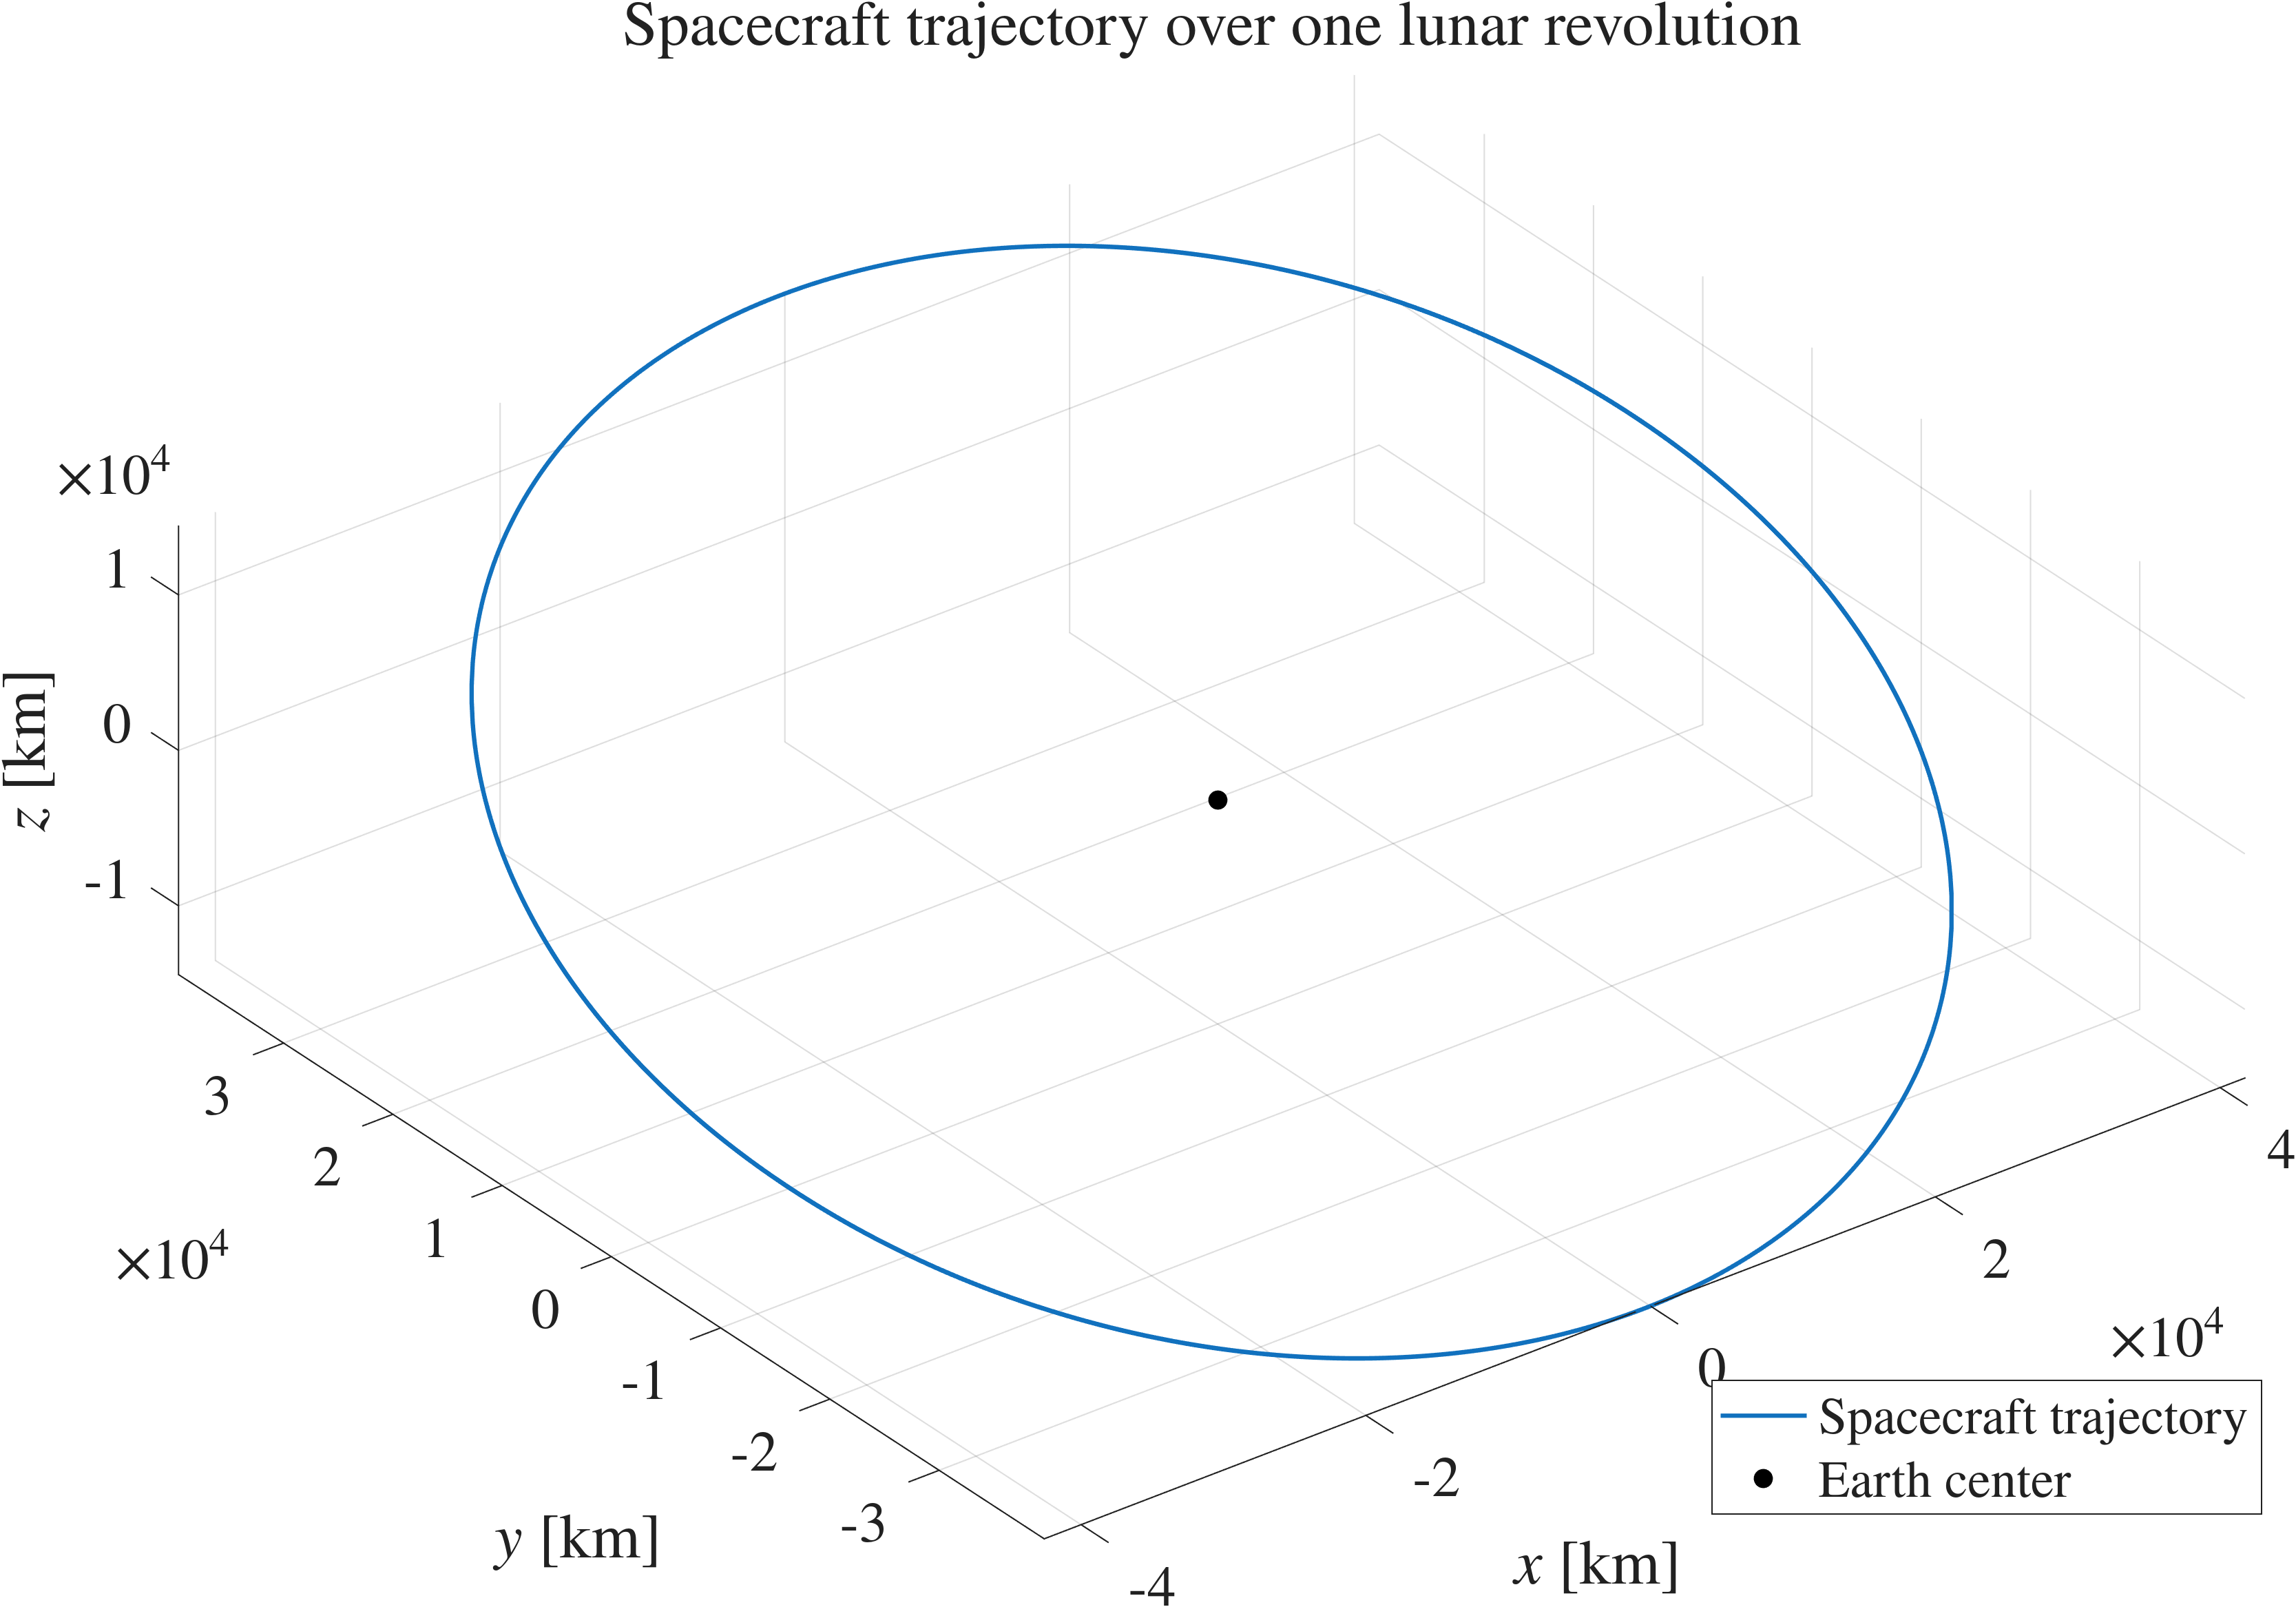
\includegraphics[width=\textwidth]{b4_trajectory_3d.png}
		\caption{3D view}
		\label{fig:b4_traj_3d}
	\end{subfigure}
	\hfill
	\begin{subfigure}{0.48\textwidth}
		\centering
		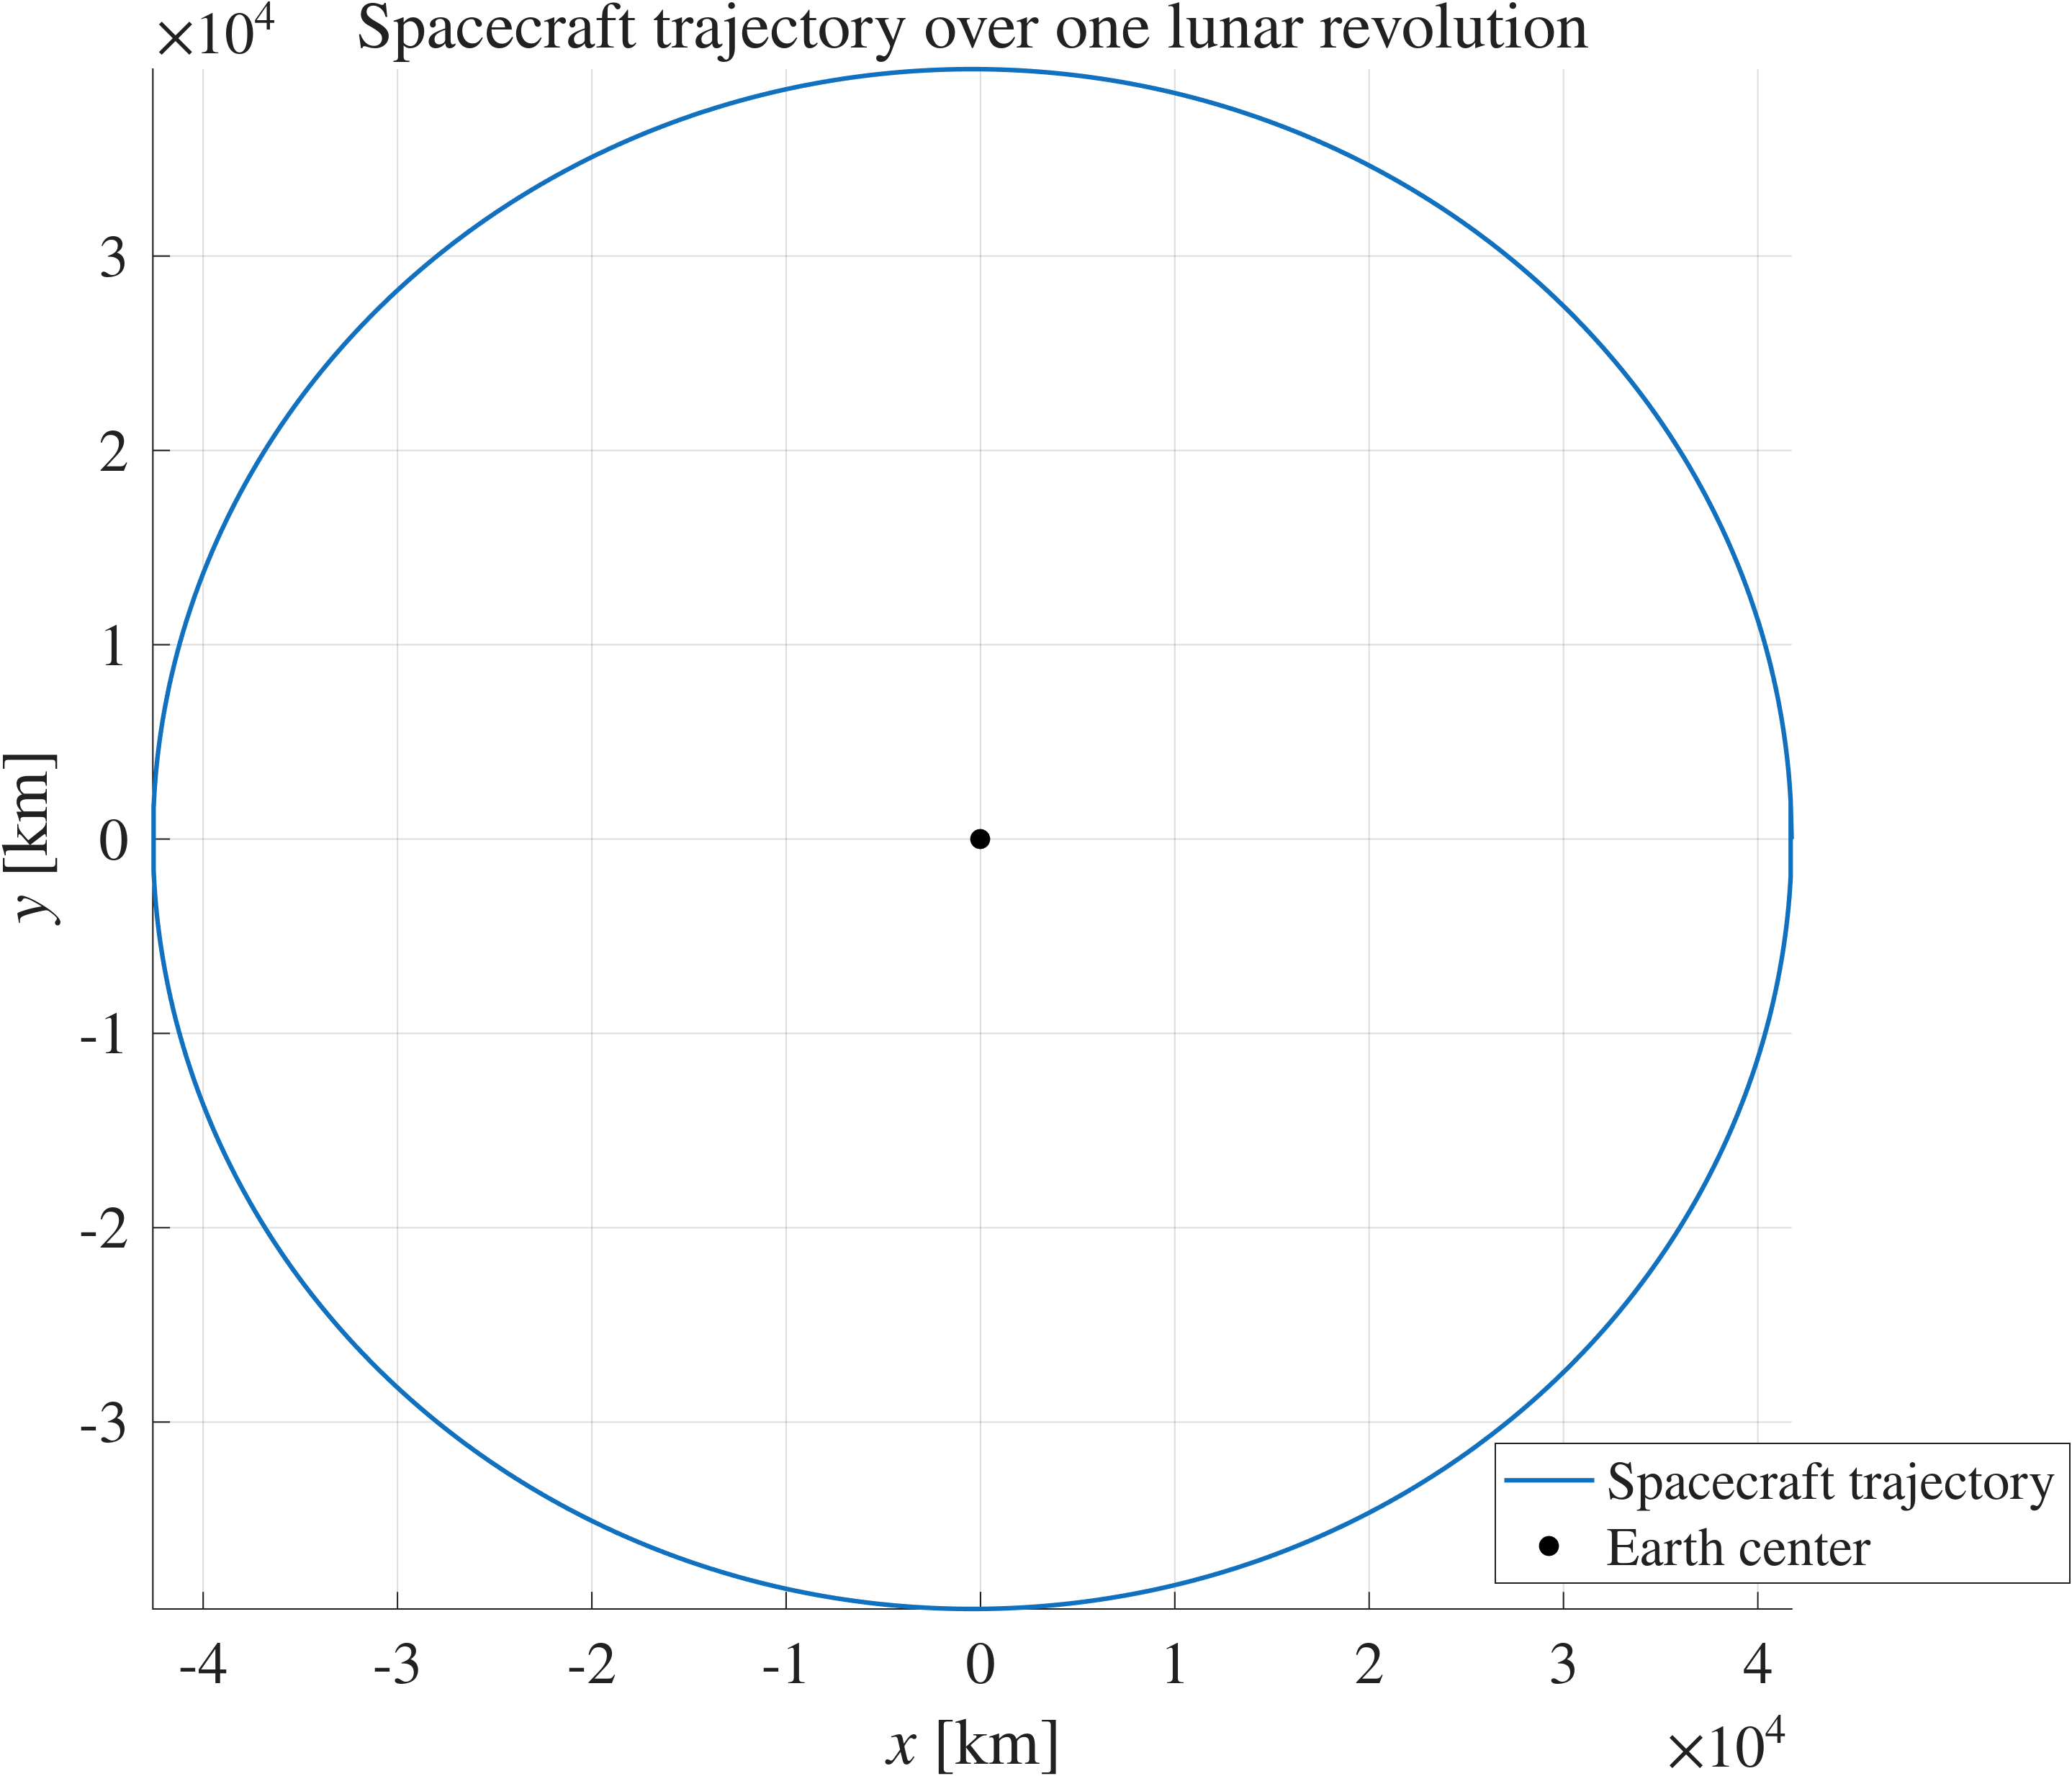
\includegraphics[width=\textwidth]{b4_trajectory_topdown.png}
		\caption{Top-down view ($x$-$y$ plane)}
		\label{fig:b4_traj_topdown}
	\end{subfigure}
	
	\begin{subfigure}{0.48\textwidth}
		\centering
		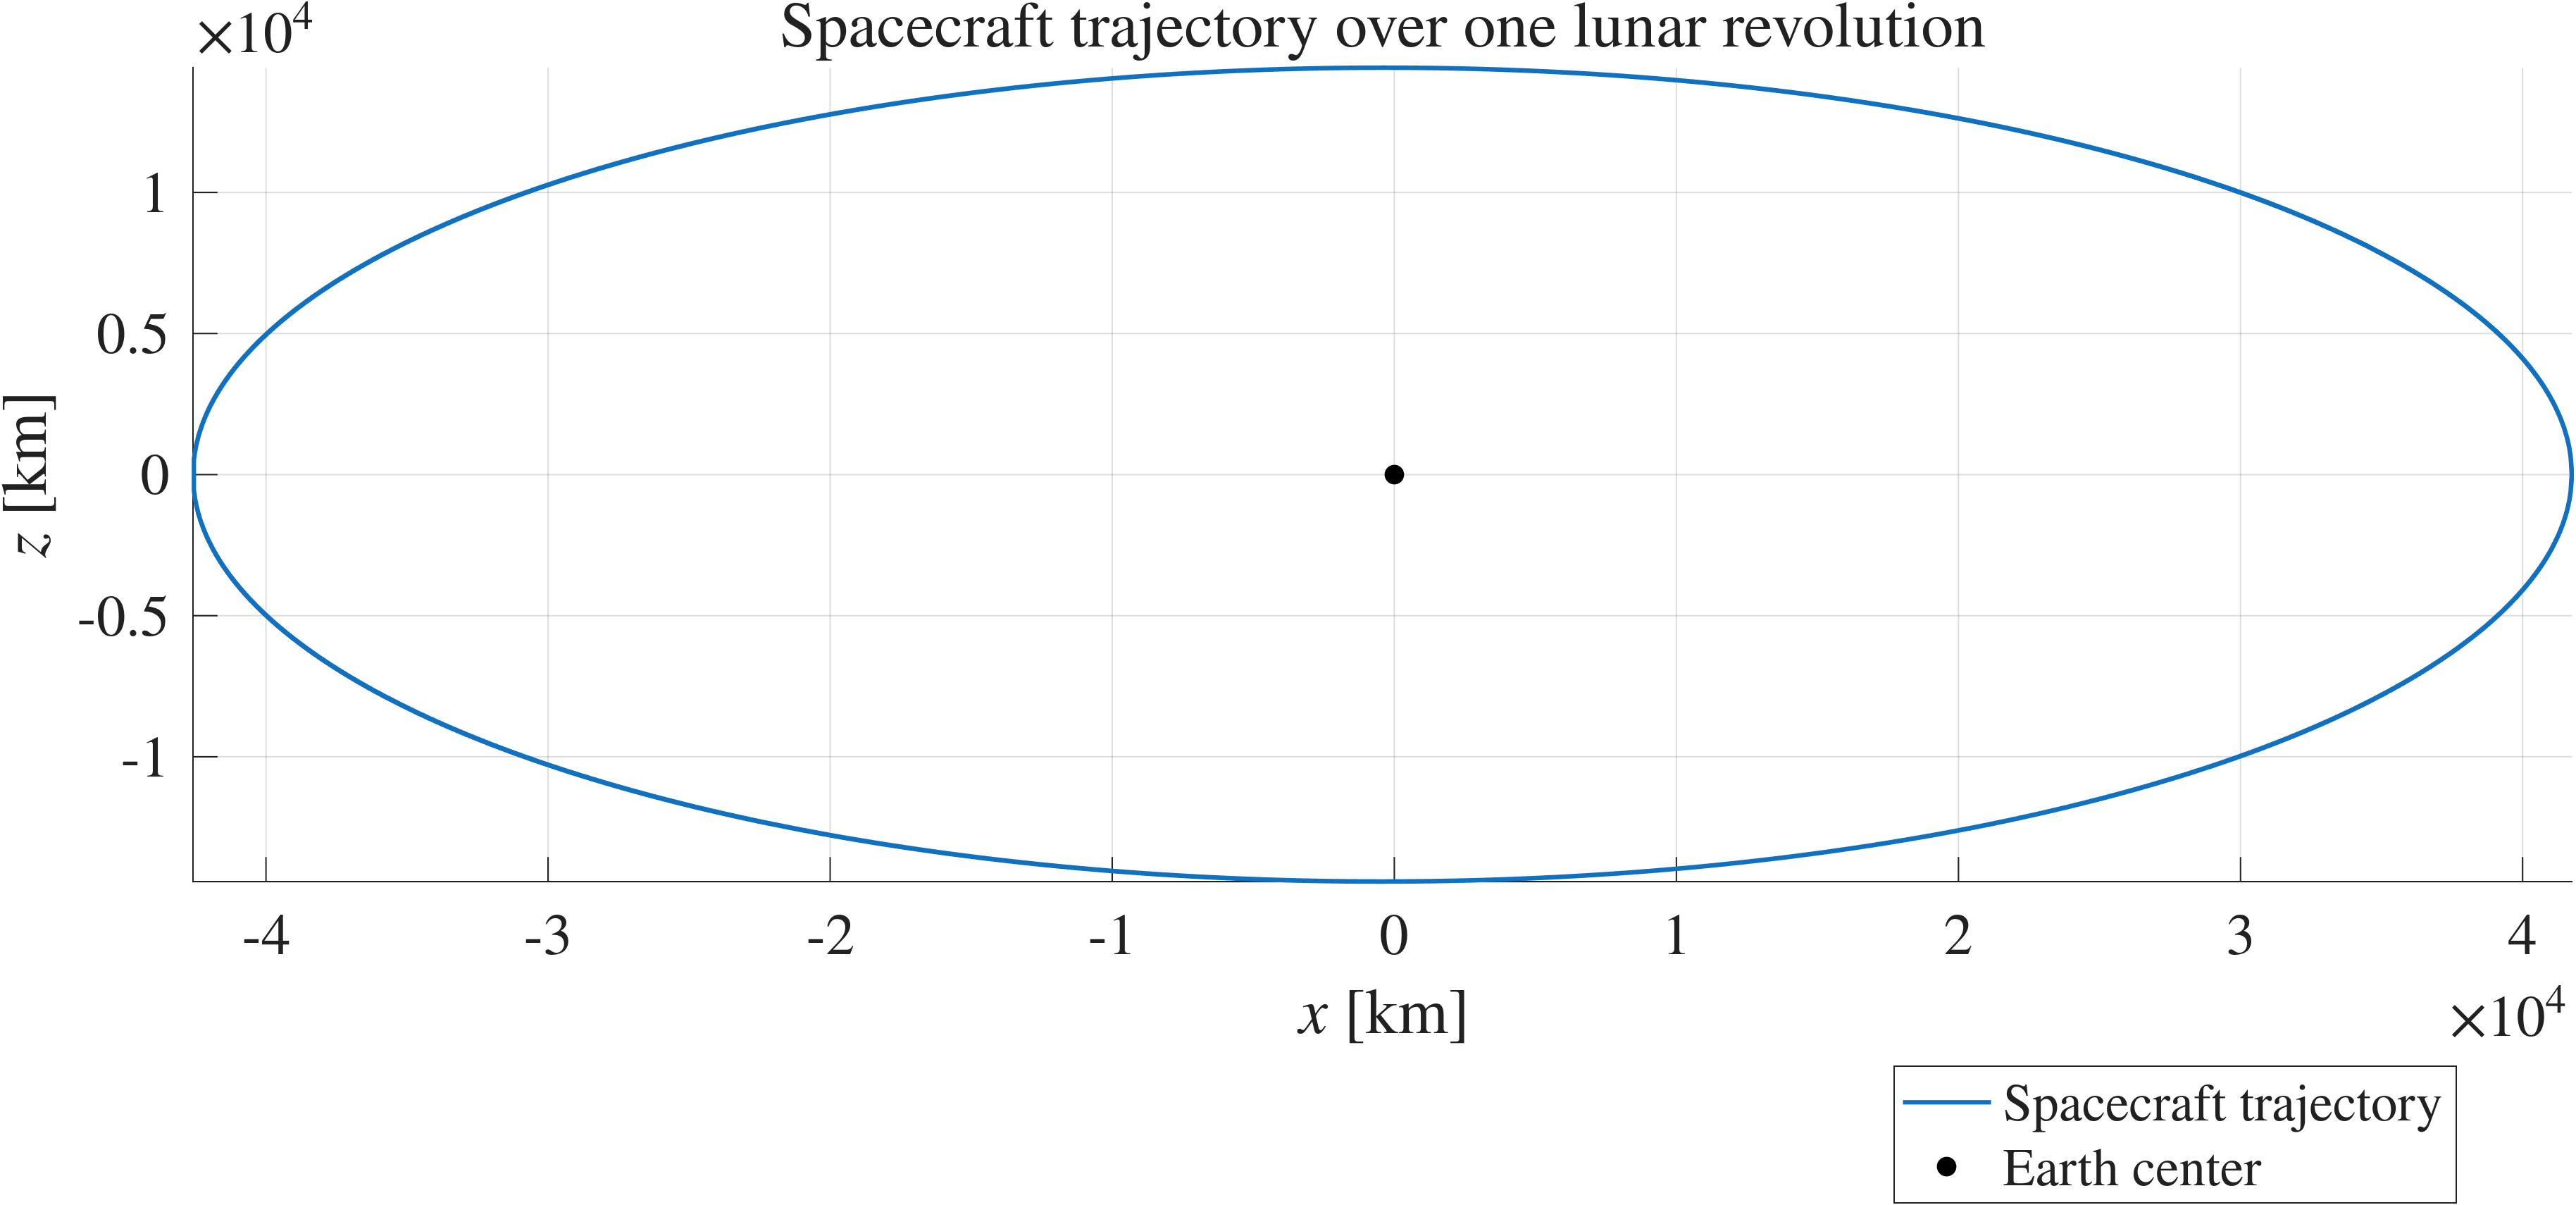
\includegraphics[width=\textwidth]{b4_trajectory_edgeon_xz.png}
		\caption{Edge-on view ($x$-$z$ plane)}
		\label{fig:b4_traj_edgeon_xz}
	\end{subfigure}
	\hfill
	\begin{subfigure}{0.48\textwidth}
		\centering
		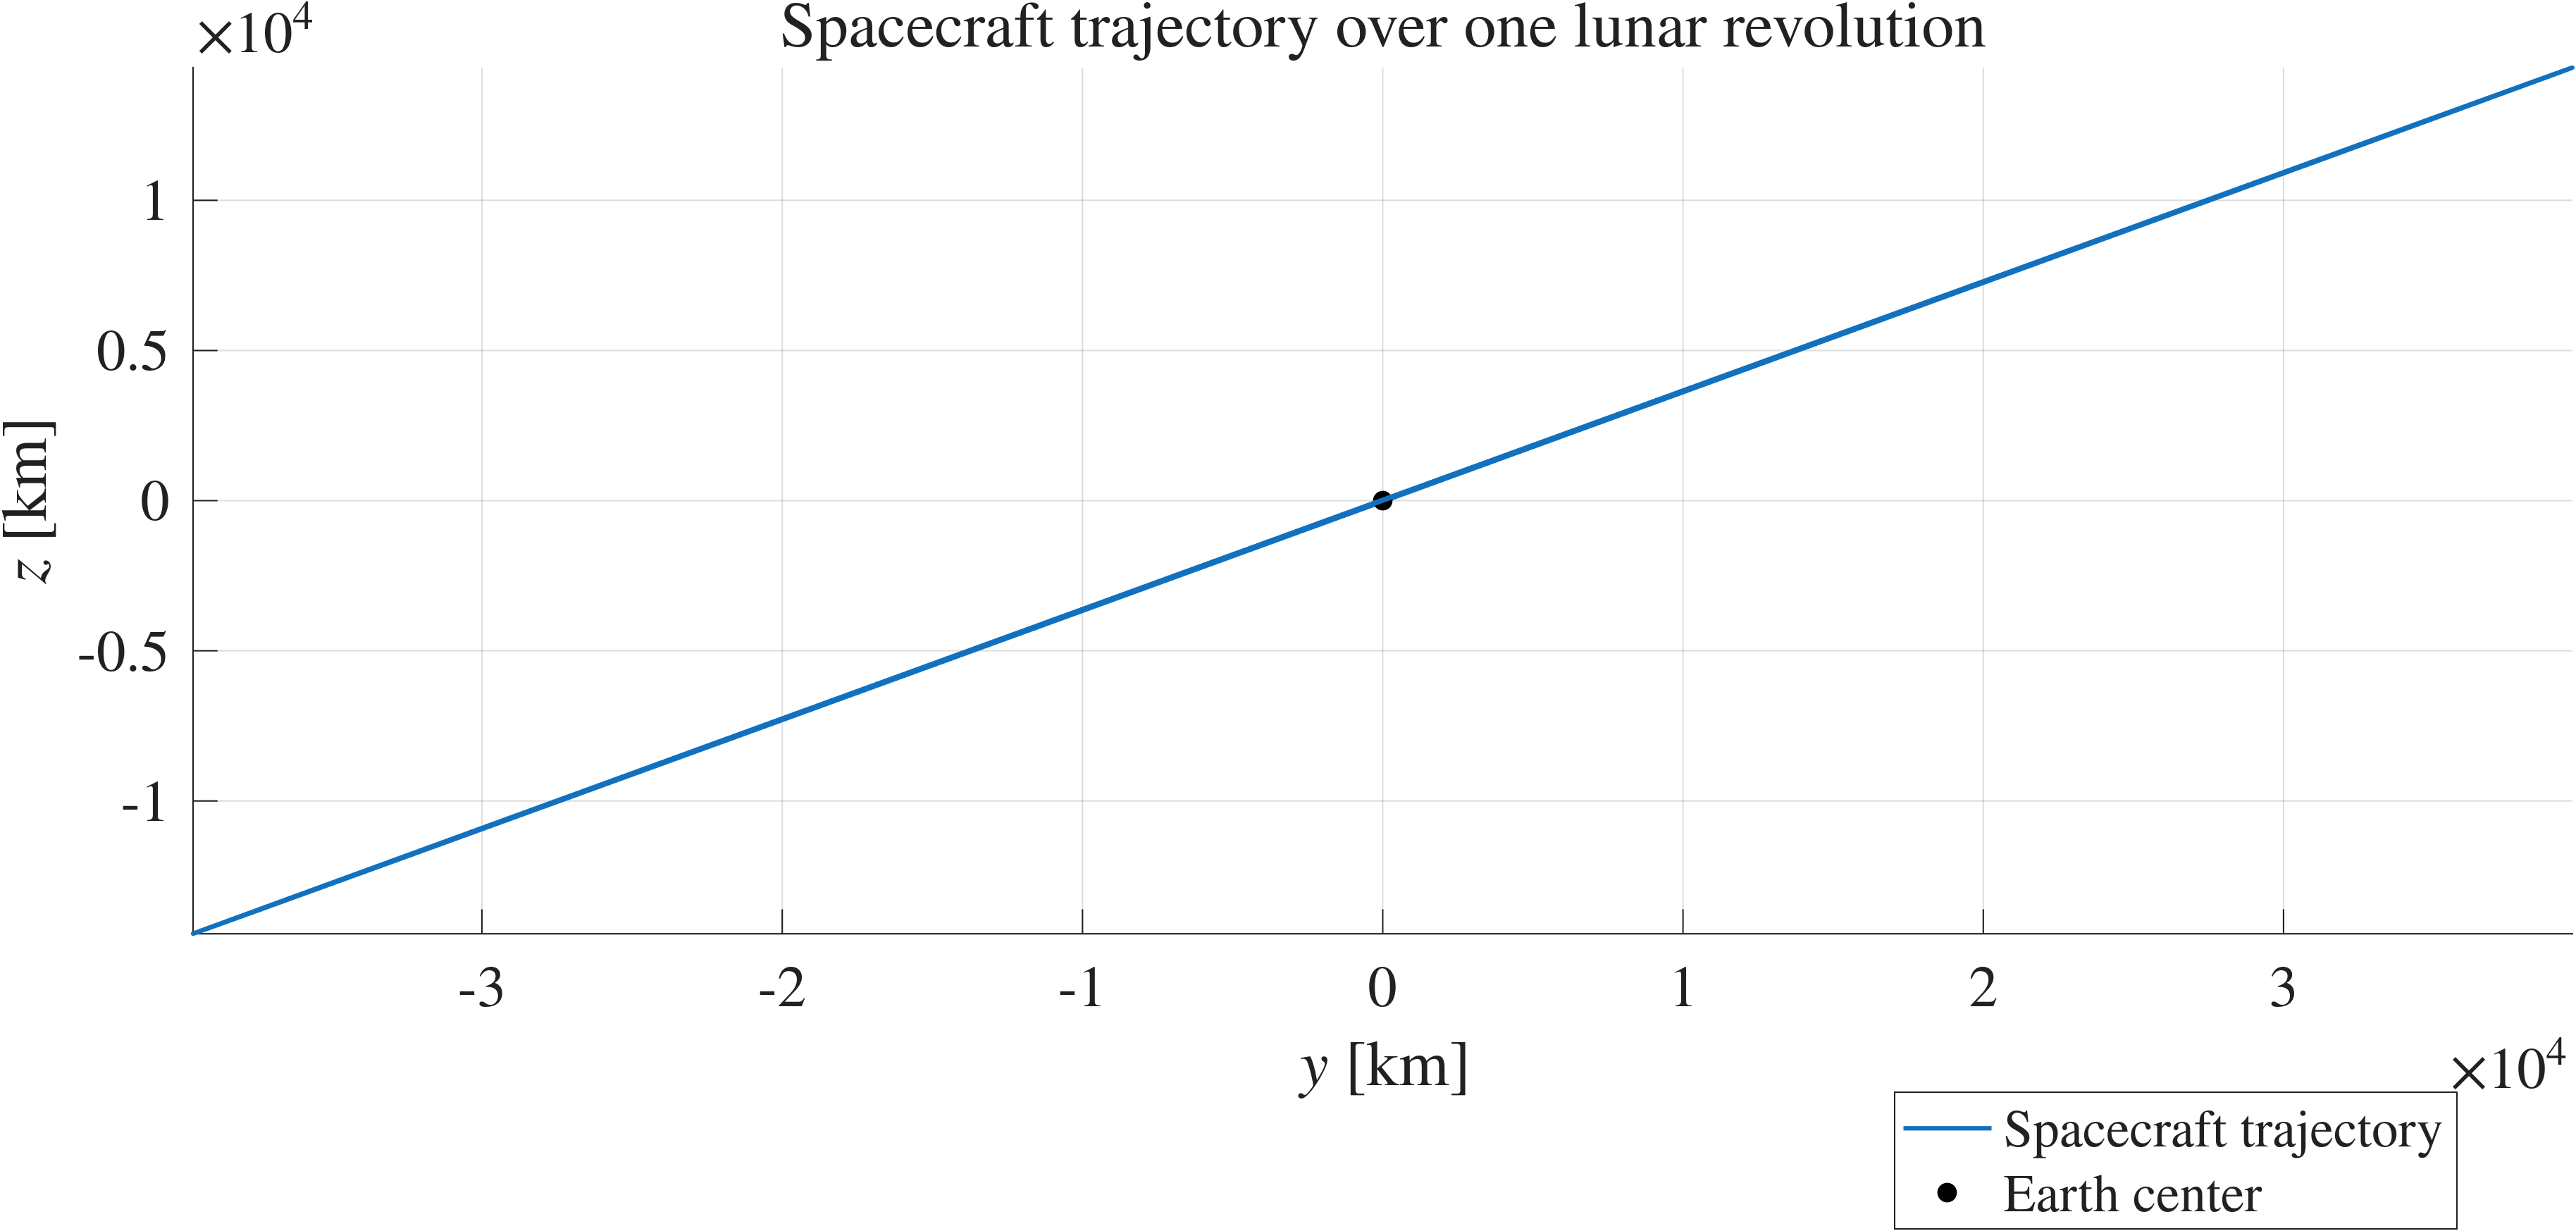
\includegraphics[width=\textwidth]{b4_trajectory_edgeon_yz.png}
		\caption{Edge-on view ($y$-$z$ plane)}
		\label{fig:b4_traj_edgeon_yz}
	\end{subfigure}
	\caption{Spacecraft trajectory in configuration space over one lunar revolution without extending the phase space.}
	\label{fig:b4_trajectory}
\end{figure}

\newpage

Plot of the time history of $\boldsymbol{q}$ coordinates:
\begin{figure}[H]
	\centering
	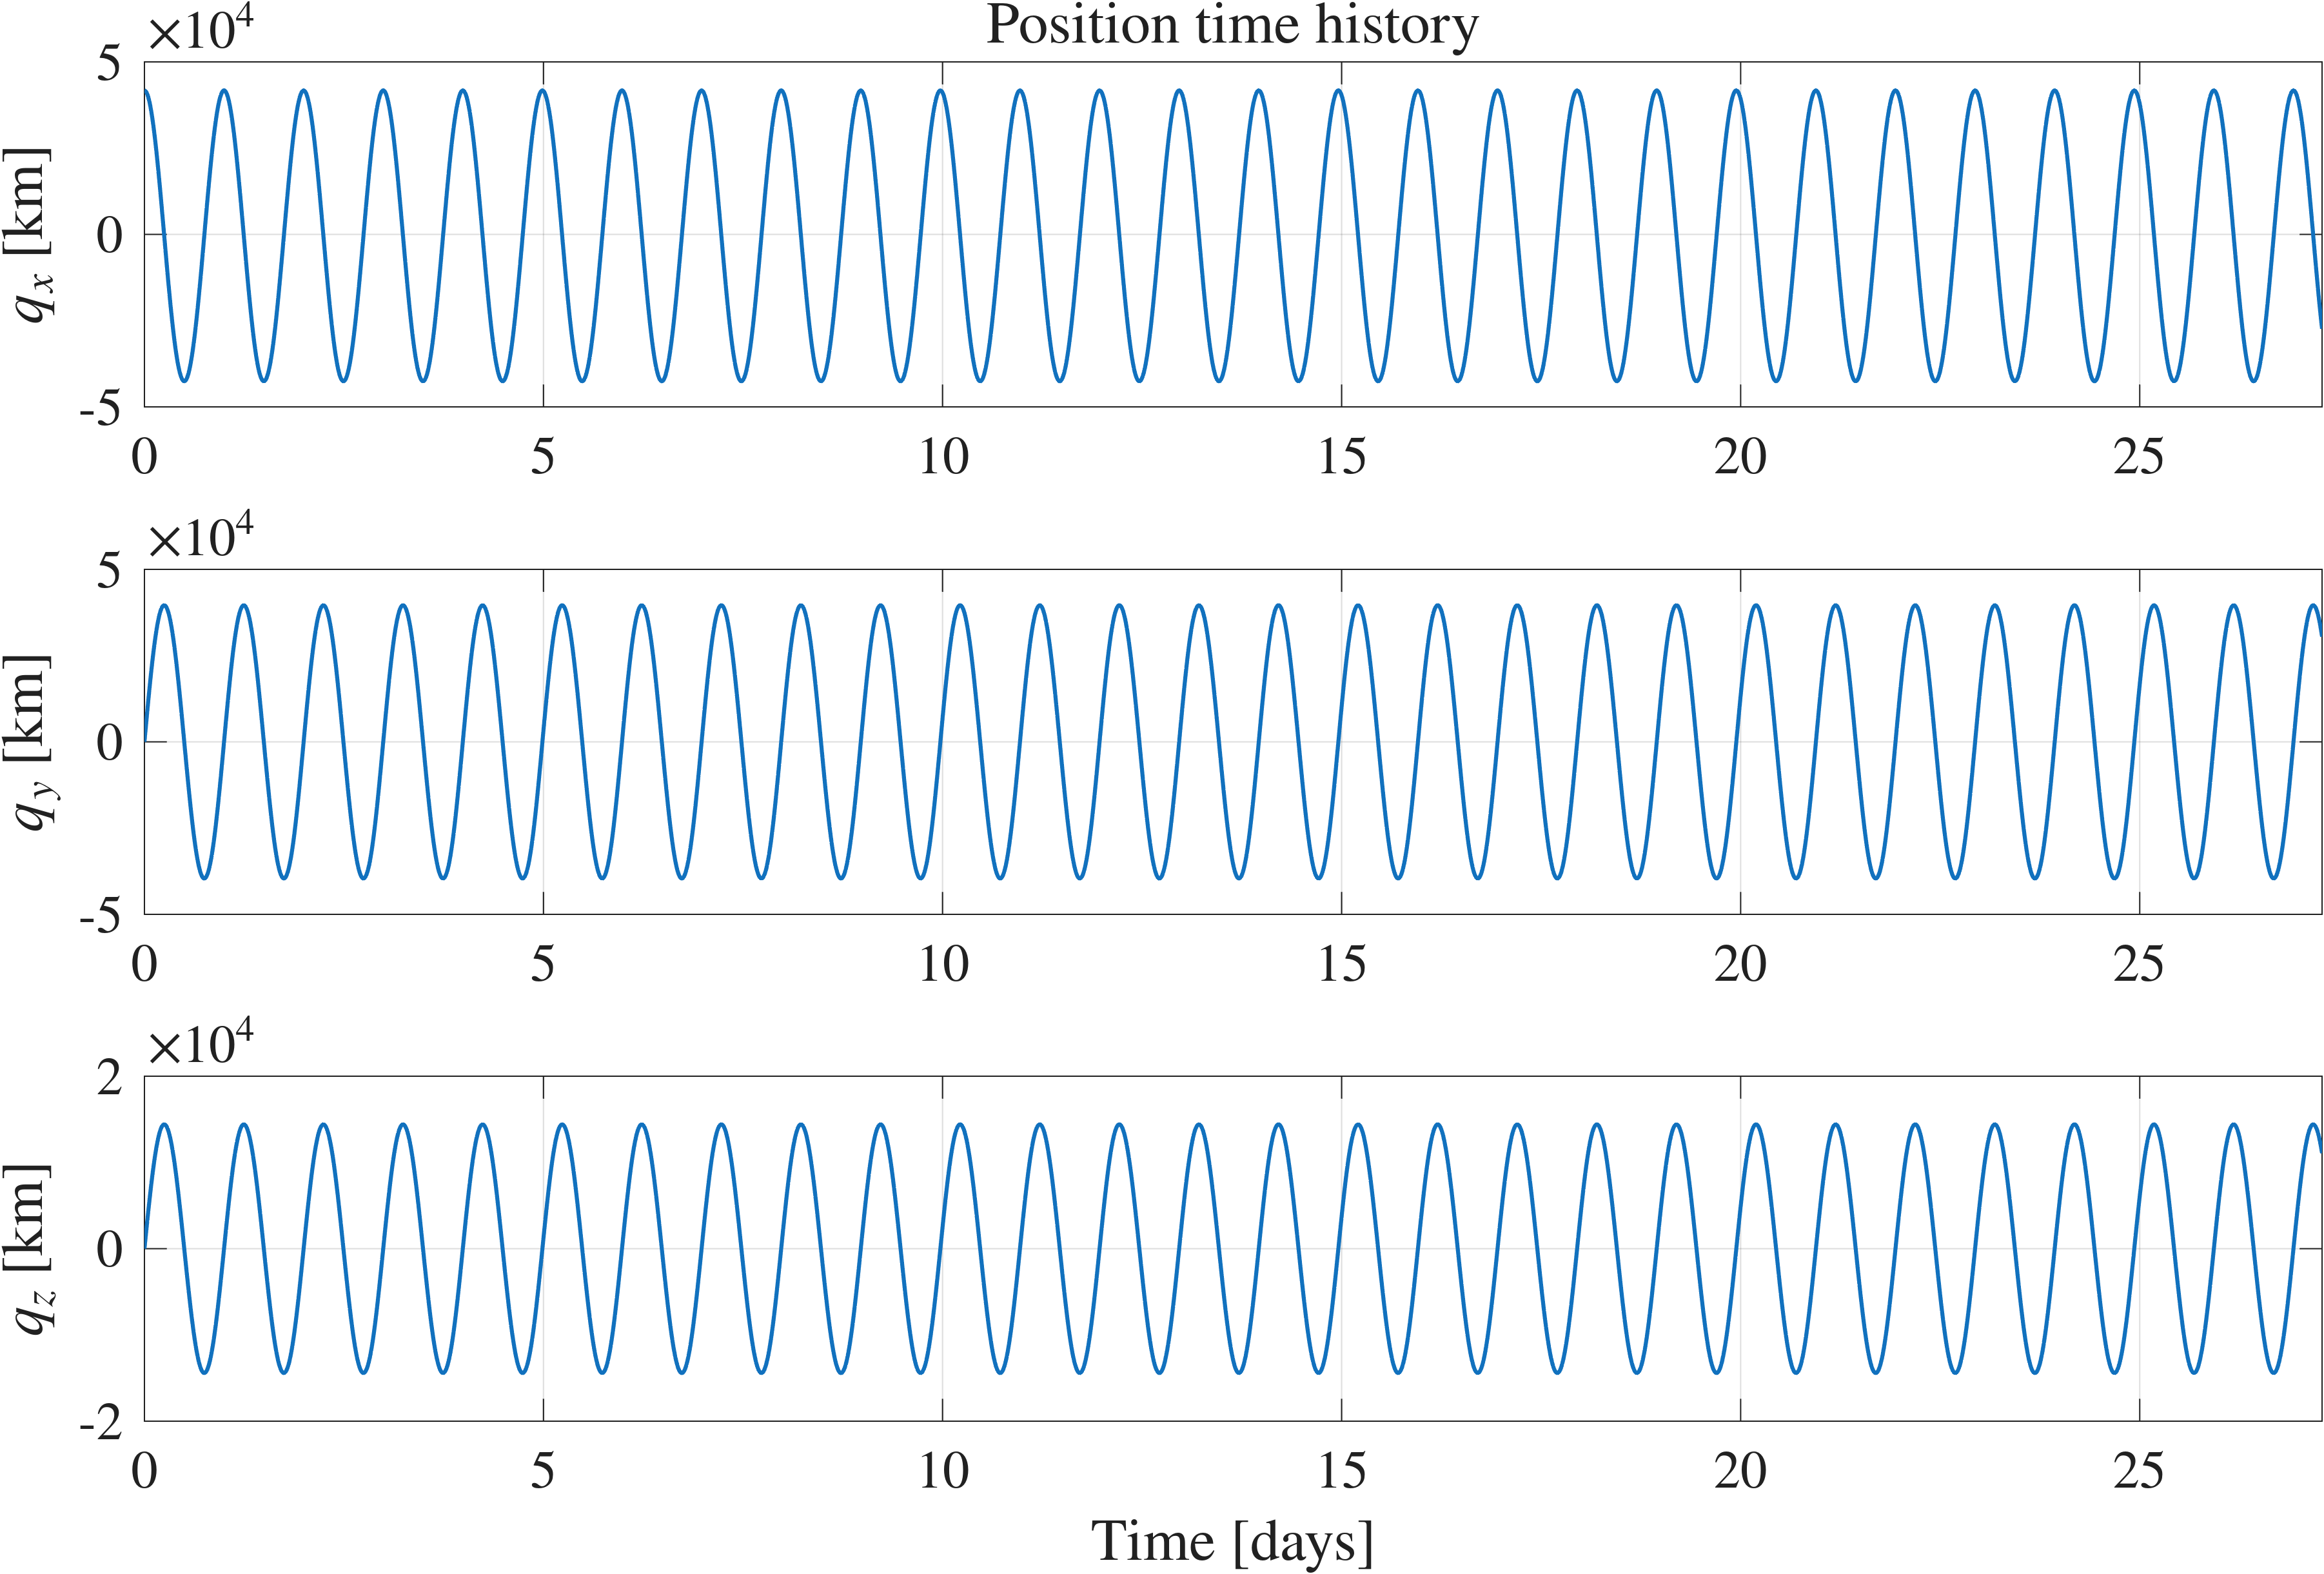
\includegraphics[width=0.9\textwidth]{b4_q.png}
	\caption{Position $\boldsymbol{q}(t)$ components over one lunar revolution without extending the phase space.}
	\label{fig:b4_q}
\end{figure}

And time history plot of their conjugate momenta $\boldsymbol{p}$:
\begin{figure}[H]
	\centering
	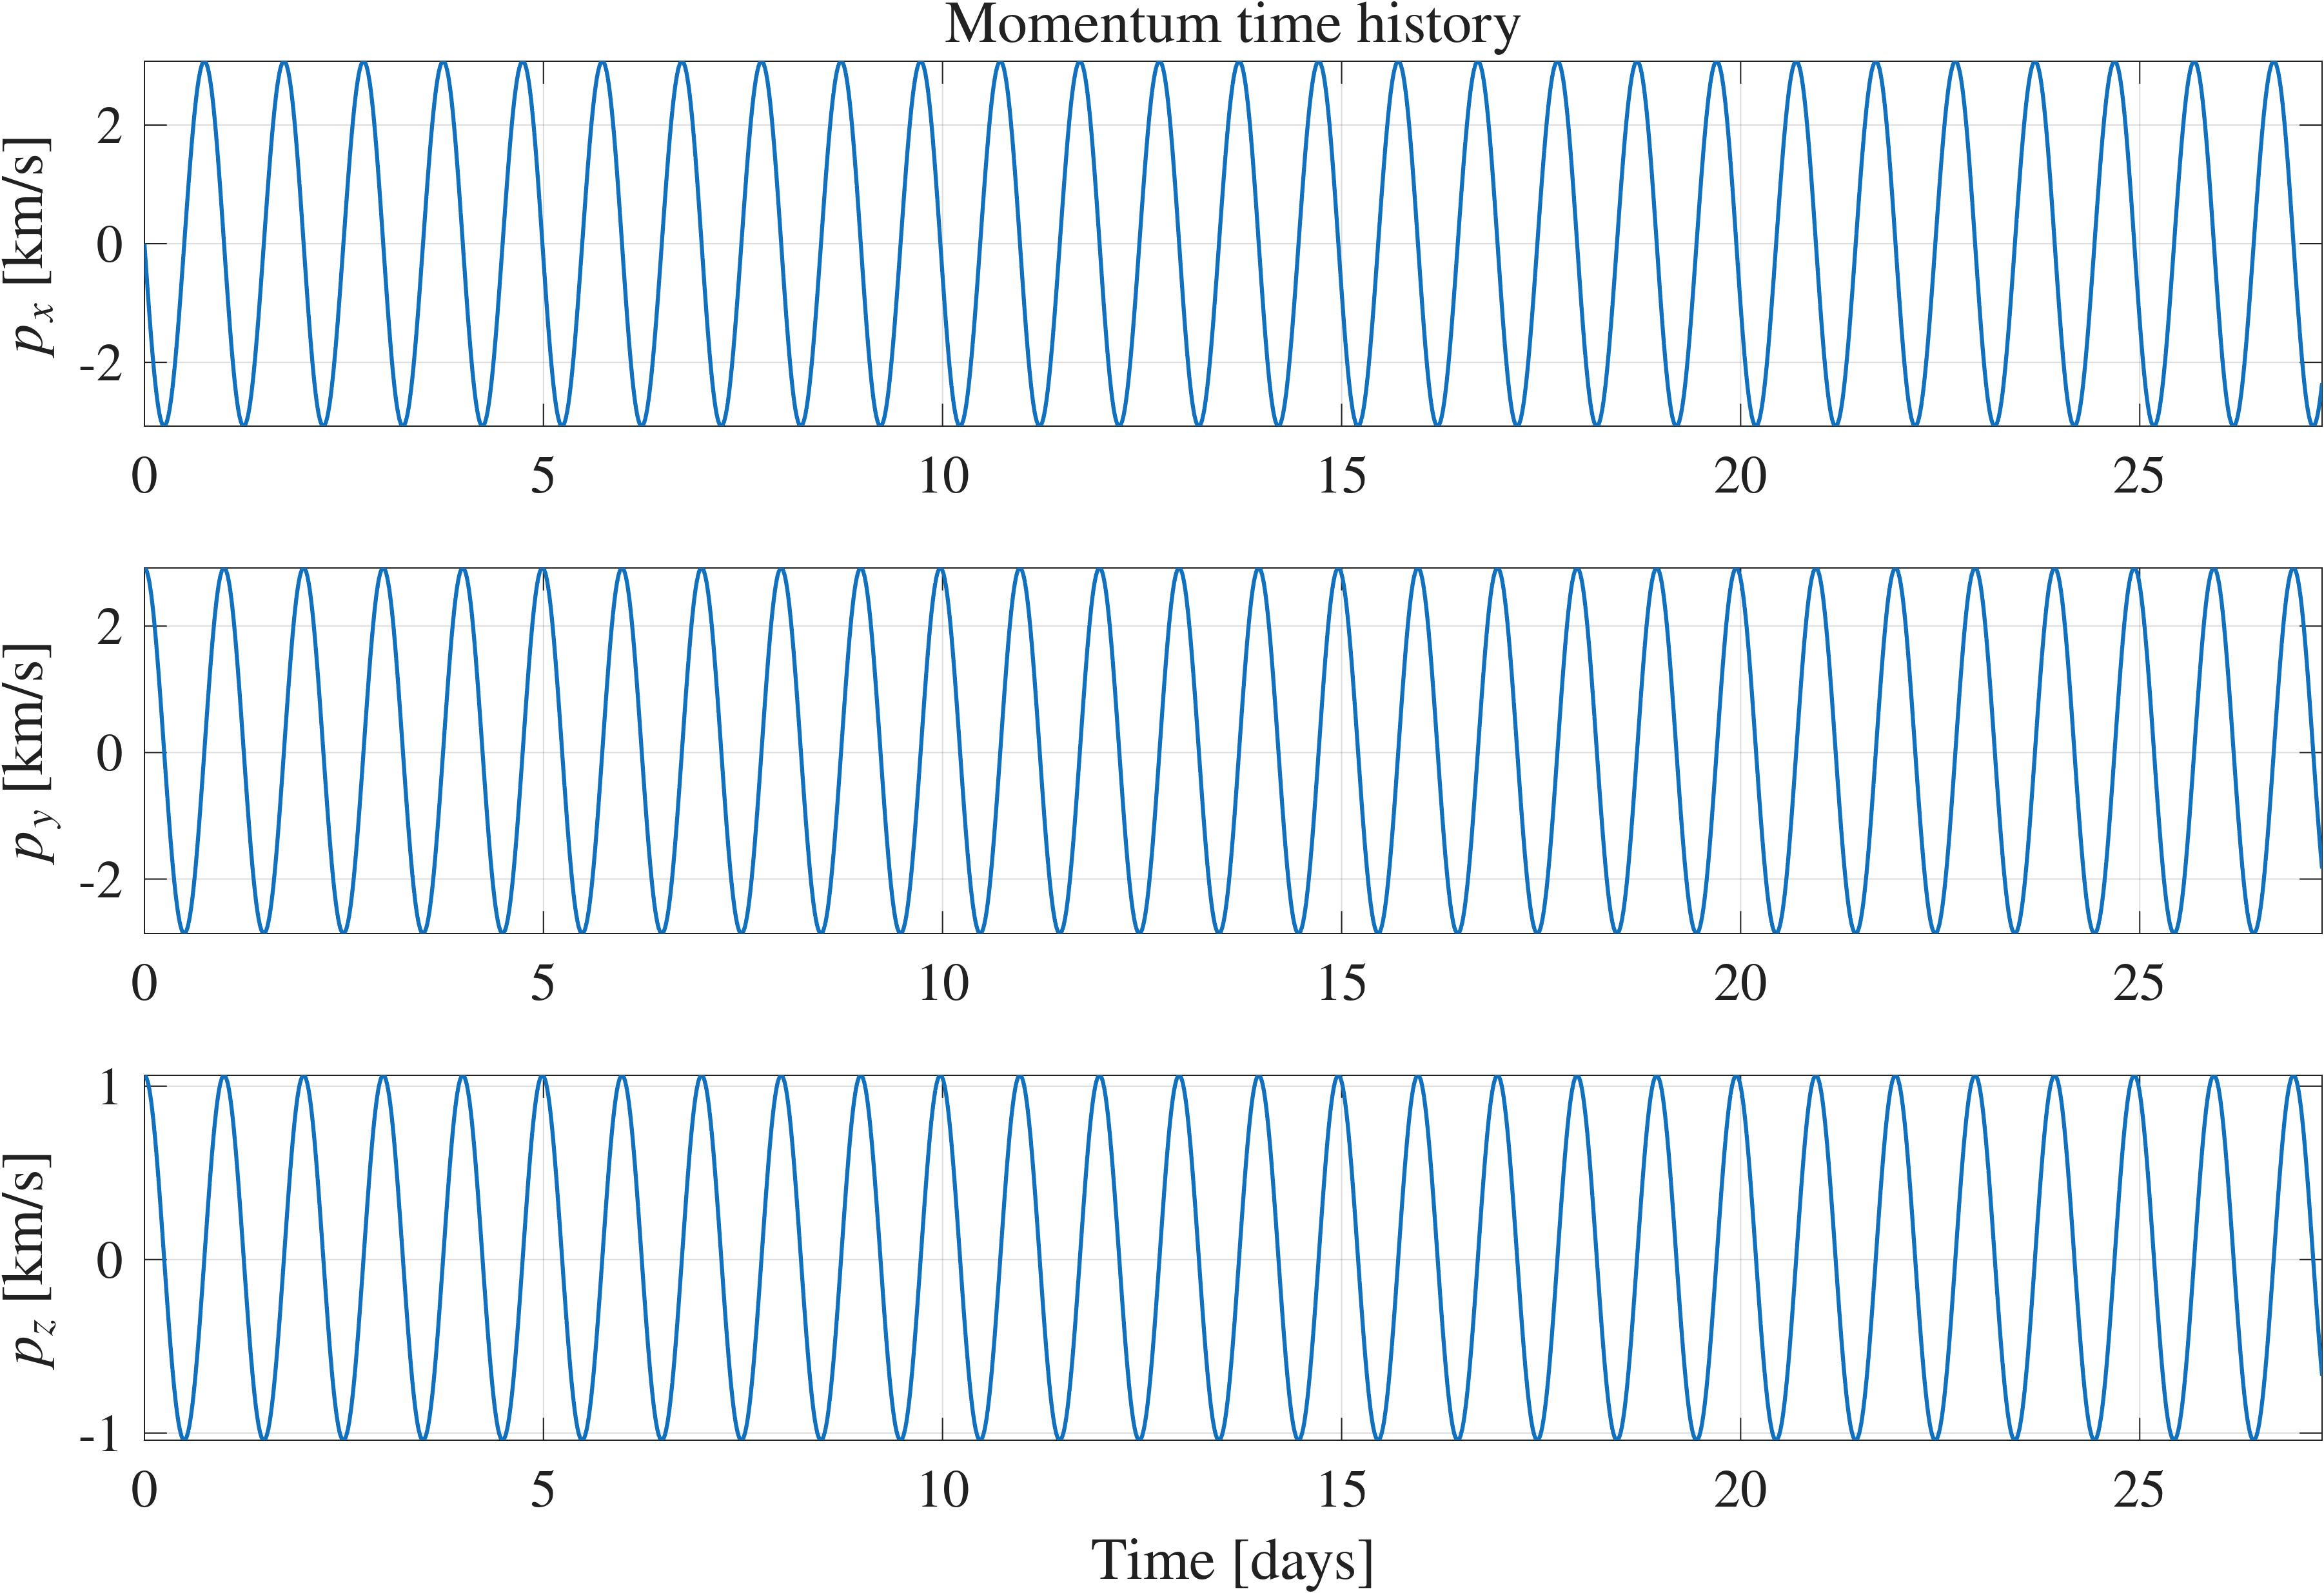
\includegraphics[width=0.9\textwidth]{b4_p.png}
	\caption{Momentum $\boldsymbol{p}(t)$ components over one lunar revolution without extending the phase space.}
	\label{fig:b4_p}
\end{figure}

The variation of the Hamiltonian $H$ from its initial state $H(0)$:
\begin{figure}[H]
	\centering
	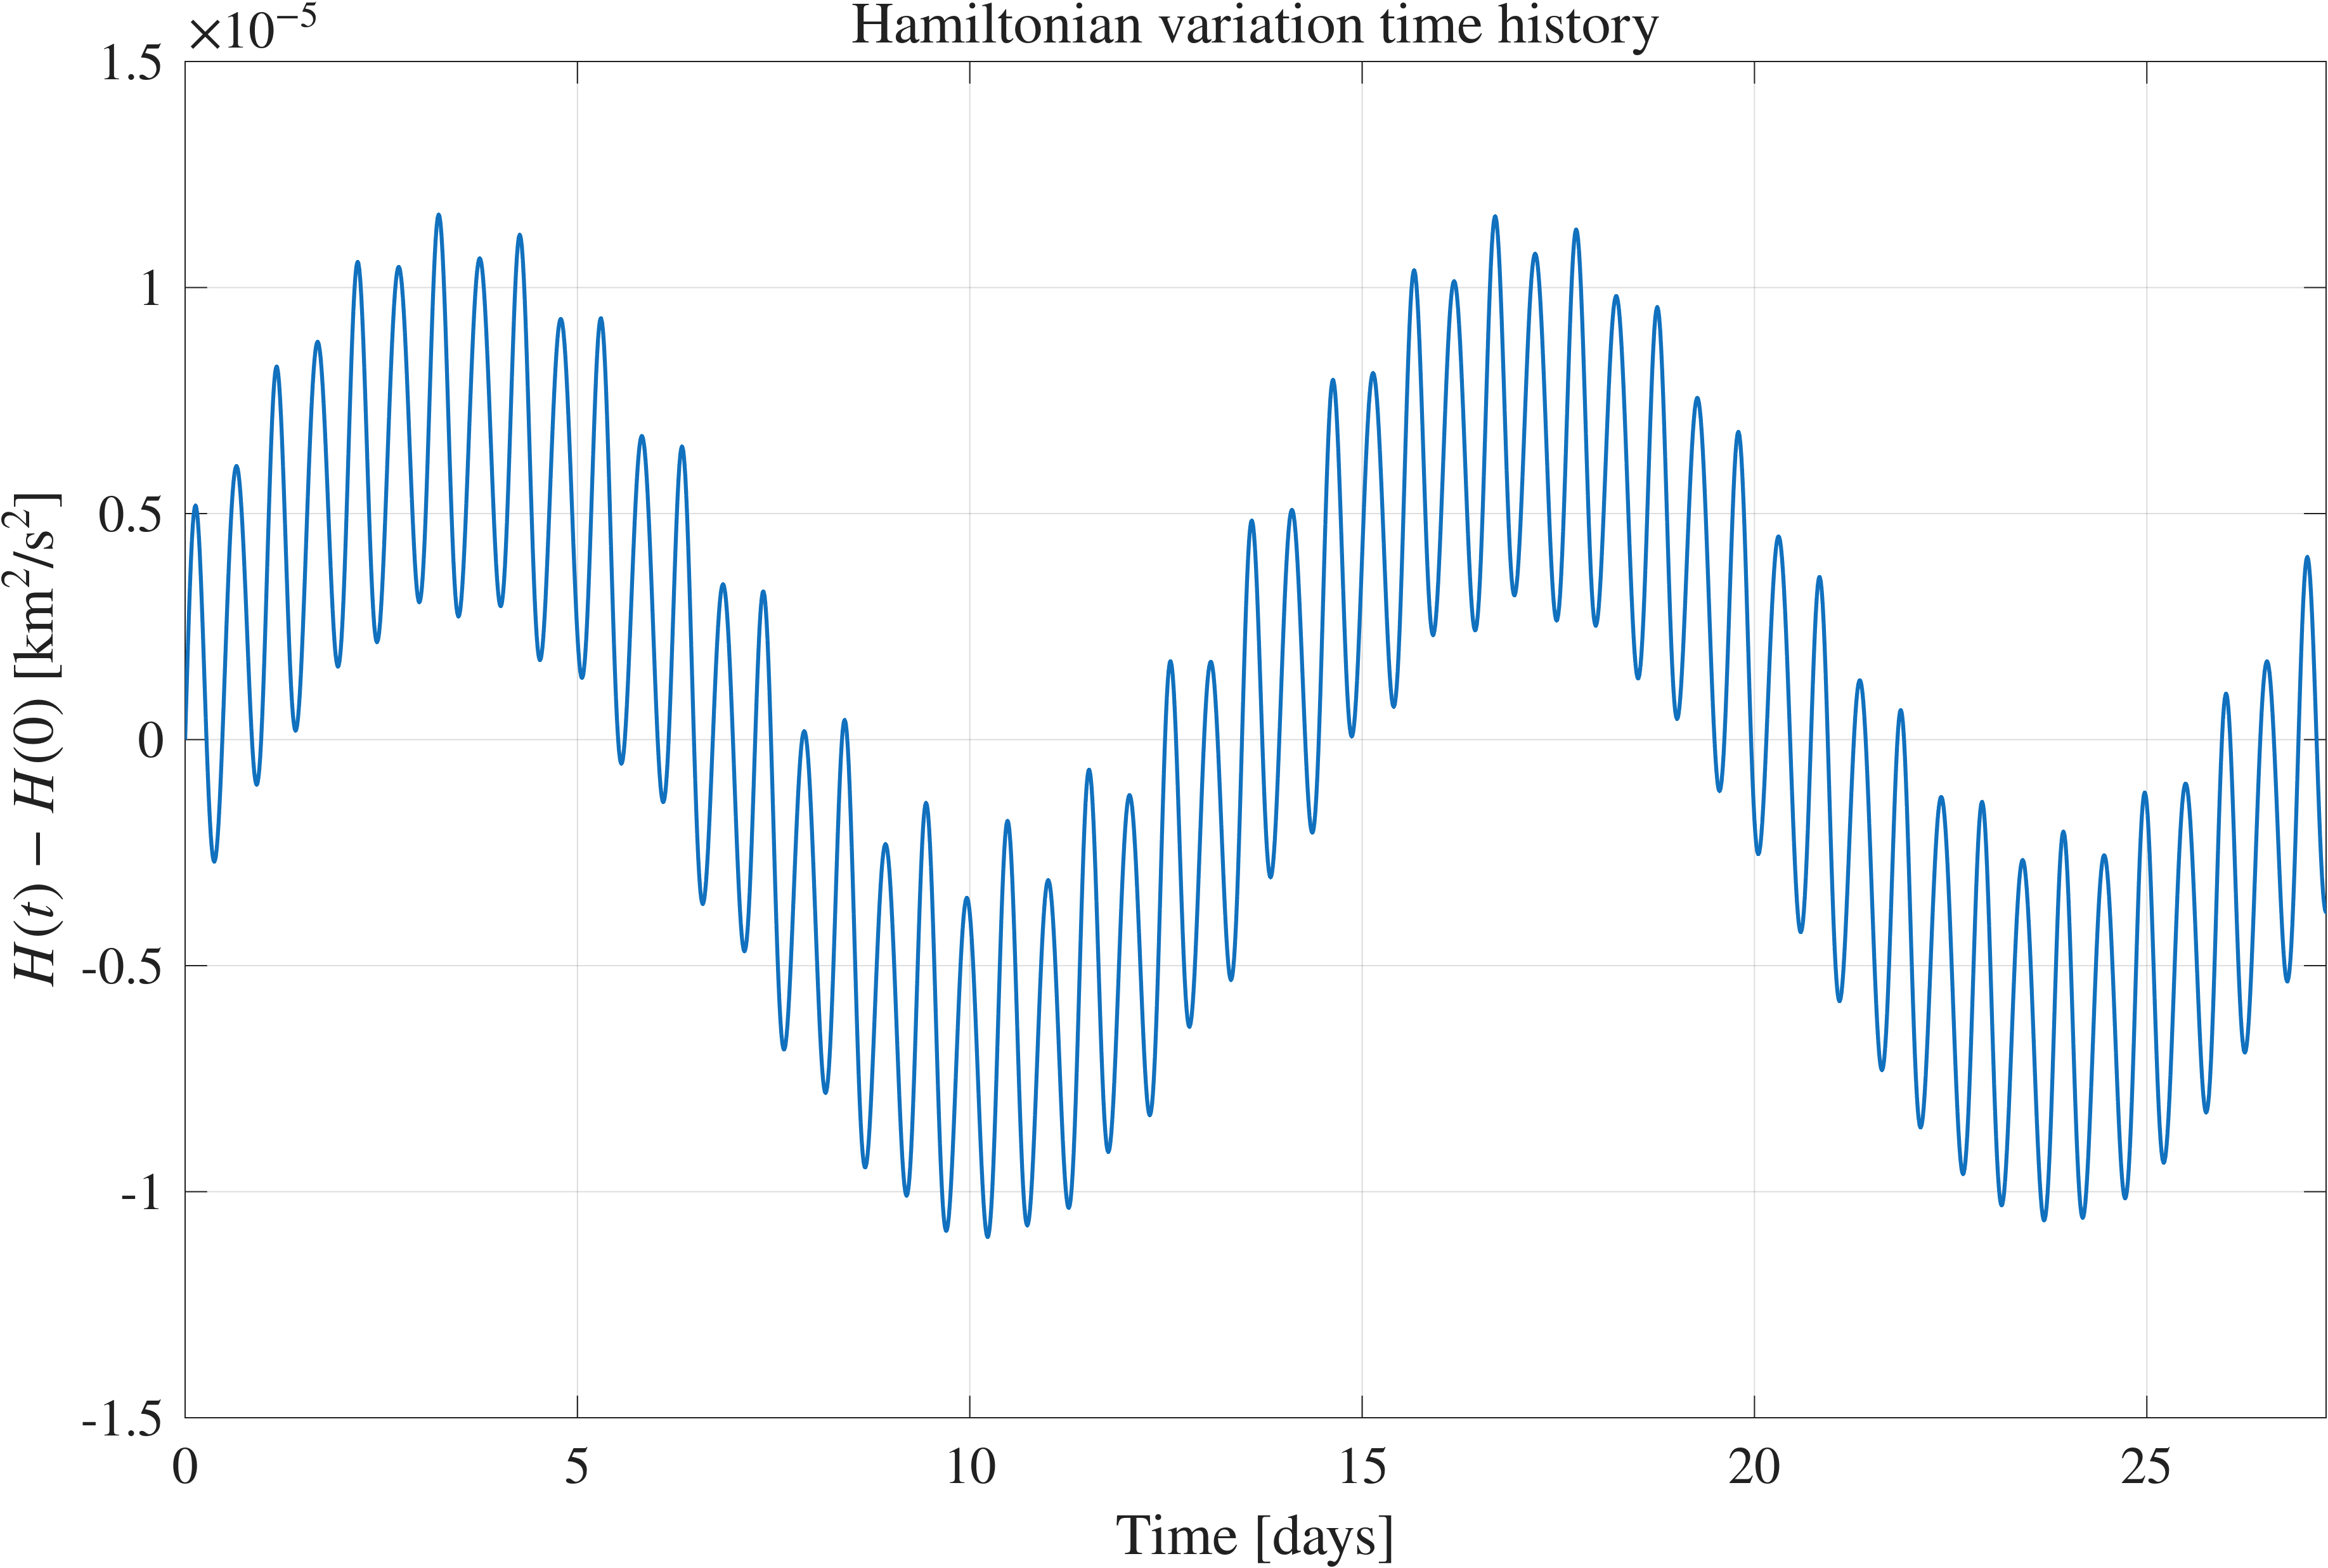
\includegraphics[width=0.9\textwidth]{b4_H.png}
	\caption{Hamiltonian variation $H(t)-H(0)$ over one lunar revolution without extending the phase space.}
	\label{fig:b4_H}
\end{figure}

And of course the $\widehat{H}$ plot is not included because the non-extended phase-space does not have an $\widehat{H}$ value. \\

We see in the above plots that the results appear identical to the extended phase-space. To confirm this, the two simulations are run on a common time grid, and the absolute value of individual $q$ and $p$ components are compared, as well as their norms:
\begin{equation}
	\begin{split}
		|\Delta q_j|&=|q_j^{\mathrm{ext}}-q_j^{\mathrm{reg}}|,\quad|\Delta p_j|=|p_j^{\mathrm{ext}}-p_j^{\mathrm{reg}}|,\quad j\in\{x,y,z\} \\
		\|\Delta\boldsymbol{q}\|_2&=\|\boldsymbol{q}^{\mathrm{ext}}-\boldsymbol{q}^{\mathrm{reg}}\|_2=\sqrt{\Delta q_x^2+\Delta q_y^2+\Delta q_z^2} \\
		\|\Delta\boldsymbol{p}\|_2&=\|\boldsymbol{p}^{\mathrm{ext}}-\boldsymbol{p}^{\mathrm{reg}}\|_2=\sqrt{\Delta p_x^2+\Delta p_y^2+\Delta p_z^2}
	\end{split}
\end{equation}
Where the superscripts ext and reg denote the extended and non-extended phase-space solutions respectively. \\

From Hamilton's equations in (b.2) and above, $\dot{\boldsymbol{q}}=\boldsymbol{p}$. Since $\boldsymbol{q}$ is the Cartesian position of the spacecraft, its time derivative is the velocity:
\begin{equation}
	\boldsymbol{p}=\dot{\boldsymbol{q}}=\boldsymbol{v}\quad\implies\quad\Delta\boldsymbol{p}=\Delta\boldsymbol{v}
\end{equation}
So the momentum differences $\Delta\boldsymbol{p}$ are directly the velocity differences requested by the problem, in units of km/s. \\

\begin{mdframed}[linewidth=1pt, innertopmargin=10pt, innerbottommargin=10pt]
	Then, the following table shows the max differences found by the program:
	\begin{table}[H]
		\centering
		\caption{Maximum differences between the extended and non-extended phase-space solutions over one lunar revolution}
		\label{tab:b4_differences}
		\begin{tabular}{|c|c|c|c|}
			\hline
			\multicolumn{2}{|c|}{Position} & \multicolumn{2}{c|}{Velocity} \\
			\hline
			Quantity & Value [km] & Quantity & Value [km/s] \\
			\hline
			$\max|\Delta q_x|$ & $1.033504\times10^{-8}$ & $\max|\Delta p_x|$ & $5.945244\times10^{-13}$ \\
			\hline
			$\max|\Delta q_y|$ & $7.443305\times10^{-9}$ & $\max|\Delta p_y|$ & $7.047696\times10^{-13}$ \\
			\hline
			$\max|\Delta q_z|$ & $2.741217\times10^{-9}$ & $\max|\Delta p_z|$ & $2.576273\times10^{-13}$ \\
			\hline
			$\max\|\Delta\boldsymbol{q}\|_2$ & $1.137470\times10^{-8}$ & $\max\|\Delta\boldsymbol{p}\|_2$ & $7.984083\times10^{-13}$ \\
			\hline
		\end{tabular}
	\end{table}
	We see that none of the differences are larger than an order of $10^{-8}$ for position, and $10^{-13}$ for velocity, which is consistent with what is expected for numerical drift. This is expected, since both share the same equations for $\dot{\boldsymbol{q}}$ and $\dot{\boldsymbol{p}}$, with the extended formulation only adding the time coordinate $q_0$ and its conjugate momentum $p_0$, which do not affect the motion of the spacecraft, and instead only provide a conserved extended Hamiltonian $\widehat{H}$.
\end{mdframed}

\subsection*{(b.5): Find}

Let $h_z=(\boldsymbol{q}\times\boldsymbol{p})\cdot\hat{\boldsymbol{e}}_z$ be the component of specific angular momentum normal to the lunar orbital plane. Using Poisson brackets in $(\boldsymbol{q},\boldsymbol{p})$, determine whether a constant $c$ exists such that $F_c=H+c\,h_z$ is conserved. Account for the explicit time dependence of $H$. \\

\textbf{Analysis/Conclusions:}\\

\end{document}